\documentclass[12pt, a4paper, reqno]{article}
\usepackage{preamble}

\title{\bf Билеты к государственному экзамену по математике \\ ФРКТ, 2024}
\date{}
\author{by \href{https://github.com/KetchuppOfficial}{KetchuppOfficial}}

\begin{document}

\nocite{petrovich-1}

\maketitle

\newpage
\tableofcontents

\newpage
\section{Принятые обозначения}

    $U_{\delta}(x_0)$ -- $\delta$-окрестность точки $x_0$.

    $\mathring U_{\delta}(x_0)$ -- проколотая $\delta$-окрестность точки $x_0$.

    $B_{\delta}(x_0)$ -- $\delta$-окрестность точки $x_0$ (только в ТФКП).

    $\mathring B_{\delta}(x_0)$ -- проколотая $\delta$-окрестность точки $x_0$ (только в ТФКП).

    $f \in R(G)$ -- функция, интегрируемая по Риману на множестве $G$.

    ПГП -- простая гладкая поверхность.

    КГП -- кусочно-гладкая поверхность.

    ОДСК -- общая декартова система координат.

    ПДСК -- прямоугольная декартова система координат.

\newpage
\section{Введение в математический анализ}

\subsection{\textit{БИЛЕТ 1}. Теорема Больцано-Вейерштрасса и критерий Коши сходимости числовой последовательности}

    \textbf{Определение}: числовой последовательностью называется функция с областью определения
    $\mathbb{N}$ и множеством значений, принадлежащим $\mathbb{R}$.

    \textbf{Определение}: $\varepsilon$-окрестностью $U_{\varepsilon}(\alpha)$ символа $\alpha$, где
    $\alpha$ -- один из 6 стандартных предельных символов $a$, $a + 0$, $a - 0$, $+\infty$, $-\infty$,
    $\infty$, называется одно из следующих 6 множеств:
    \begin{enumerate}
        \item $U_{\varepsilon}(a) = (a - \varepsilon; a + \varepsilon)$;
        \item $U_{\varepsilon}(a + 0) = [a; a + \varepsilon)$;
        \item $U_{\varepsilon}(a - 0) = (a - \varepsilon; a]$;
        \item $U_{\varepsilon}(+\infty) = (\varepsilon; +\infty)$;
        \item $U_{\varepsilon}(-\infty) = (-\infty; -\varepsilon)$;
        \item $U_{\varepsilon}(\infty) = (-\infty; -\varepsilon)\cup(\varepsilon; +\infty)$,
    \end{enumerate}
    где $a\in\mathbb{R}$, $\varepsilon > 0$.

    \textbf{Определение предела числовой последовательности}: символ $\alpha$ называется пределом
    числовой последовательности $x_n$, если
    \begin{equation*}
    \forall \varepsilon > 0 \hookrightarrow \exists n_0(\varepsilon)\in\mathbb{N}:
    \forall n \geq n_0 \hookrightarrow x_n\in U_{\varepsilon}(\alpha)
    \end{equation*}
    Обозначение предела: $\lim\limits_{n\to\infty} x_n = \alpha$.

    \textbf{Определение}: последовательность, имеющая конечный предел, называется сходящейся;
    последовательность, не имеющая конечного предела, называется расходящейся.

    \textbf{Определение}: пусть $x_n$ -- числовая последовательность, а $n_k$ -- строго возрастающая
    последовательность натуральных чисел; тогда последовательность $y_k = x_{n_k}$ называется
    подпоследовательностью последовательности $x_n$.

    \textbf{Определение}: число $a\in\mathbb{R}$ (или символ $+\infty$, $-\infty$) называется
    частичным пределом (предельной точкой) последовательности $x_n$, если существует такая строго
    возрастающая последовательность индексов $n_k$, что $\lim\limits_{k\to\infty} x_{n_k} = a$.

    \textbf{Лемма}: если $\lim\limits_{n\to\infty} x_n = \alpha$, где $\alpha$ -- один из 6 СПС, то
    $\forall x_{n_k} \hookrightarrow \lim\limits_{k\to\infty} x_{n_k} = \alpha$.

    $\square$ По определению предела вне любой окрестности $U_{\varepsilon}(\alpha)$ содержится не
    более конечного числа членов $x_n$. Так как все $n_k$ различны, то вне любой
    $U_{\varepsilon}(\alpha)$ имеется не более конечного числа членов $x_{n_k} \implies
    \lim\limits_{k\to\infty} x_{n_k} = \alpha$. $\blacksquare$

    \textbf{Следствие}: если  $\lim\limits_{n\to\infty} x_n = a\in\mathbb{R}$, то $a$ -- единственный
    частичный предел $x_n$.

    $\square$ Так как все подпоследовательности имеют один и тот же предел, то он является единственным
    частичным пределом. $\blacksquare$

    \textbf{Критерий частичного предела}: пусть $\alpha$ -- один из символов $a$, $+\infty$, $-\infty$;
    тогда $\alpha$ является частичным пределом $\iff$ в любой $U_{\varepsilon}(\alpha)$ содержится
    бесконечно много членов $x_n$.

    $\square$ $\boxed{\Rightarrow}$ Если $\alpha$ -- частичный предел $x_n$, то существует подпоследовательность
    $x_{n_k}: \lim\limits_{k\to\infty} x_{n_k} = \alpha$. Тогда $\forall \varepsilon > 0$ внутри
    $U_{\varepsilon}(\alpha)$ содержатся все $x_{n_k}$, начиная с некоторого номера $k_0$, а значит,
    бесконечно много членов $x_n$.

    $\boxed{\Leftarrow}$ Сначала рассмотрим случай $a\in\mathbb{R}$. Возьмём $\varepsilon = 1$, $x_{n_1}$
    -- некоторый член $x_n$ из $U_{1}(a)$. Возьмём теперь $\varepsilon = \dfrac{1}{2}$. Так как в
    $U_{\frac{1}{2}}(a)$ бесконечно много членов, то выберем $x_{n_2}\in U_{\frac{1}{2}}(a)$ так,
    что $n_2 > n_1$, и т.д. Пусть построены $x_{n_1}, x_{n_2}, \ldots, x_{n_k}$, где
    $n_1 < n_2 < \ldots < n_k$, $x_{n_k}\in U_{\frac{1}{k}}(a)$. Так как в $U_{\frac{1}{k+1}}(a)$
    бесконечно много членов $x_n$, то выберем $x_{k+1}\in U_{\frac{1}{k+1}}(a)$ так, чтобы
    $n_{k+1} > n_k$. Таким образом, построена бесконечная последовательность $x_{n_k}$, причём
    $n_1 < n_2 < \ldots < n_k < \ldots$, $\forall k\in\mathbb{N} \hookrightarrow x_{n_k}\in U_{\frac{1}{k}}(a)$.
    То есть $\forall k\in\mathbb{N} \hookrightarrow a - \dfrac{1}{k} < x_{n_k} < a + \dfrac{1}{k}$.
    По теореме о двух милиционерах: $\lim\limits_{k\to\infty} x_{n_k} = a$, то есть $a$ -- частичный
    предел $x_n$.

    Для $\alpha = +\infty$ и $\alpha = -\infty$ доказательство аналогично. Например, для
    $\alpha = +\infty$ нужно брать $\varepsilon = 1, 2, 3, \ldots, k, \ldots$; $x_{n_k}$ выбирать таким,
    что $x_{n_k}\in U_{k}(+\infty)$, то есть $x_{n_k} > k$. Тогда по аналогу теоремы о двух
    милиционерах для бесконечно больших последовательностей $\lim\limits_{k\to\infty} x_{n_k} =
    +\infty$. $\blacksquare$

    \textbf{Теорема Больцано-Вейерштрасса}: любая ограниченная последовательность имеет сходящуюся
    подпоследовательность (то есть имеет конечный частичный предел).

    $\square$ Пусть $\forall n\in\mathbb{N} \hookrightarrow a \leq x_n \leq b$, где $a < b$,
    $a, b \in\mathbb{R}$. Выберем ту половину $\left[a; \dfrac{a + b}{2}\right]$ или
    $\left[\dfrac{a + b}{2}; b\right]$ отрезка $[a; b]$ (назовём её $\Delta_1$), где содержится
    бесконечно много $x_n$ (в обеих половинах конечного числа быть не может, так как в таком случае
    весь отрезок содержит конечное число членов последовательности, что неверно). Если обе половины
    содержат бесконечно много членов $x_n$, то $\Delta_1$ -- любая из половин. На отрезке $\Delta_1$
    аналогично выбираем половину $\Delta_2$, содержащую бесконечно много членов $x_n$, и т.д. На
    $k$-м шаге в $\Delta_k$ выбираем половину $\Delta_{k+1}$, содержащую бесконечно много членов
    $x_n$. Имеем последовательность вложенных отрезков $\Delta_1 \supset \Delta_2 \supset \ldots\supset
    \Delta_n \supset \ldots$, причём длина $n$-го отрезка $|\Delta_n| = \dfrac{b-a}{2^n}$ стремится
    к нулю: $\lim\limits_{n\to\infty} |\Delta_n| = 0$.
    По теореме Кантора о вложенных отрезка, $\exists! c: \forall n\in\mathbb{N} \hookrightarrow
    c\in\Delta_n$. Отсюда следует:
    \begin{equation*}
        \forall\varepsilon > 0 \hookrightarrow \exists n_0(\varepsilon)\in\mathbb{N}: \forall n \geq
        n_0 \hookrightarrow |\Delta_n| < \varepsilon \implies
        \forall n \geq n_0 \hookrightarrow \Delta_n \subset U_{\varepsilon}(c)
    \end{equation*}
    Значит, $U_{\varepsilon}(c)$ содержит бесконечно много членов $x_n$ $\implies$ по критерию
    частичного предела, $c$ -- частичный предел $x_n$. $\blacksquare$

    \textbf{Аналог теоремы Больцано-Вейерштрасса для неограниченных последовательностей}: если
    последовательность $x_n$ неограниченна сверху, то она имеет частичный предел $+\infty$; если
    последовательность $x_n$ неограниченна снизу, то она имеет частичный предел $-\infty$.

    $\square$ Докажем первую часть теоремы. Вторая доказывается аналогично.

    Зафиксируем $E > 0$. $x_n$ неограниченна сверху $\implies \exists n_1(E)\in\mathbb{N}: x_{n_1} > E$.
    Теперь в качестве нового $E$ в определении неограниченности сверху рассмотрим $x_{n_1}$. Тогда
    $\exists n_2(x_{n_1})\in\mathbb{N}: x_{n_2} > x_{n_1}$ и т.д. Мы выбрали бесконечно много
    различных членов последовательности $x_n$ таких, что

    $x_{n_1} < x_{n_2} < \ldots < x_{n_k} < \ldots$ и $\forall k\in\mathbb{N} \hookrightarrow
    x_{n_k}\in U_{E}(+\infty) \implies$ по критерию частичного предела, $+\infty$ -- частичный предел
    последовательности $x_n$. $\blacksquare$

    \textbf{Теорема о единственном частичном пределе}: пусть последовательность $x_n$ ограничена и
    имеет единственный частичный предел, равный $a$; тогда $\lim\limits_{n\to\infty} x_n = a$.\\
    $\square$ Пусть $\forall n\in\mathbb{N} \hookrightarrow m \leq x_n \leq M$, где $m < M$,
    $m, M\in\mathbb{R}$. Так как для некоторой подпоследовательности
    $x_{n_k} \hookrightarrow \lim\limits_{k\to\infty} x_{n_k} = a$ и
    $\forall k \in \mathbb{N} \hookrightarrow m \leq x_{n_k} \leq M$, то по теореме о предельном
    переходе в неравенстве: $m \leq a \leq M$.

    Докажем, что $\exists\lim\limits_{n\to\infty} x_n = a$. Если это не так, то
    $\exists\varepsilon > 0:$ вне $U_{\varepsilon}(a)$ содержится бесконечно много членов $x_n$.
    Пусть для определённости бесконечно много членов $x_n$ справа от $U_{\varepsilon}(a)$, то есть
    на $[a + \varepsilon; M]$. По теореме Больцано-Вейерштрасса, на $[a + \varepsilon; M]$
    существует частичный предел $x_n$, отличный от $a$, -- противоречие. $\blacksquare$

    \textbf{Определение}: последовательность $x_n$ называется фундаментальной, если
    \begin{equation*}
        \forall\varepsilon > 0 \hookrightarrow \exists n_0(\varepsilon)\in\mathbb{N}: \forall n, m
        \geq n_0 \hookrightarrow |x_n - x_m| < \varepsilon
    \end{equation*}

    \textbf{Критерий Коши сходимости последовательности}: последовательность $x_n$ сходится $\iff$
    $x_n$ фундаментальна.

    $\square$ $\boxed{\Rightarrow}$ Пусть $\lim\limits_{n\to\infty} x_n = a\in\mathbb{R}$; тогда
    \begin{equation*}
        \forall\varepsilon > 0 \hookrightarrow \exists n_1(\varepsilon)\in\mathbb{N}: \forall n \geq
        n_1 \hookrightarrow |x_n - a| < \dfrac{\varepsilon}{2}
    \end{equation*}
    \begin{equation*}
        \forall\varepsilon > 0 \hookrightarrow \exists n_2(\varepsilon)\in\mathbb{N}: \forall m \geq
        n_2 \hookrightarrow |x_m - a| < \dfrac{\varepsilon}{2}
    \end{equation*}
    Тогда $\forall n, m \geq n_0 = \max(n_1, n_2)$ выполняется
    \begin{equation*}
        |x_n - x_m| = |x_n - a + a - x_m| \leq |x_n - a| + |x_m - a| < \dfrac{\varepsilon}{2} +
        \dfrac{\varepsilon}{2} = \varepsilon.
    \end{equation*}
    Значит, последовательность $x_n$ фундаментальна.

    $\boxed{\Leftarrow}$ Пусть $x_n$ -- фундаментальная последовательность. Докажем сначала, что она
    ограничена. При $\varepsilon = 1$ имеем
    \begin{equation*}
        \exists n_0(1)\in\mathbb{N}: \forall n, m \geq n_0 \hookrightarrow |x_n - x_m| < 1
    \end{equation*}
    Зафиксируем $m = n_0$. Тогда
    \begin{equation*}
        \forall n \geq n_0 \hookrightarrow |x_n| = |x_n - x_m + x_m| \leq |x_n - x_m| + |x_m| <
        1 + |x_m| = 1 + |x_{n_0}|
    \end{equation*}
    Таким образом, последовательность $x_n$ ограничена при $n \geq n_0 \implies x_n$ ограничена.

    По теореме Больцано-Вейерштрасса последовательность $x_n$ имеет конечный частичный предел. В
    силу теоремы о единственном частичном пределе достаточно доказать, что других частичных пределов
    последовательность не имеет. Предположим, что это не так и существуют два различных частичных
    предела $a$ и $b$ (для определённости $a < b$). Возьмём в определении фундаментальности
    $\varepsilon = \dfrac{b - a}{3}$. Тогда для данного $\varepsilon$:
    \begin{equation*}
        \exists n_0\left(\dfrac{b - a}{3}\right)\in\mathbb{N}: \forall n, m \geq n_0
        \hookrightarrow|x_n - x_m| < \dfrac{b - a}{3}
    \end{equation*}
    В $U_{\varepsilon}(a)$ содержится бесконечно много членов $x_n$ по критерию частичного предела.
    Значит:
    \begin{equation*}
        \exists n_1\in\mathbb{N}: n_1 \geq n_0,\ x_{n_1}\in U_{\varepsilon}(a)
    \end{equation*}
    Аналогично:
    \begin{equation*}
        \exists n_2\in\mathbb{N}: n_2 \geq n_0,\ x_{n_2}\in U_{\varepsilon}(b)
    \end{equation*}
    Тогда $|x_{n_1} - x_{n_2}| > \dfrac{b - a}{3}$ -- противоречие определению фундаментальности.
    $\blacksquare$

\newpage
\subsection{\textit{БИЛЕТ 2}. Ограниченность функции, непрерывной на отрезке, достижение точной верхней и нижней
            граней}

    \textbf{Определение}: пусть функция $f$ определена в некоторой окрестности точки
    $a\in\mathbb{R}$; тогда $f$ называется непрерывной в точке $a$, если
    $\exists\lim\limits_{x\to a} f(x) = f(a)$.

    \textbf{Определение}: пусть функция $f$ определена в некоторой окрестности $a + 0$ (или
    $a - 0$), $a\in\mathbb{R}$; тогда $f$ называется непрерывной справа (соответственно слева) в
    точке $a$, если $\exists\lim\limits_{x\to a + 0} f(x) = f(a)$ (соответственно
    $\exists\lim\limits_{x\to a - 0} f(x) = f(a)$).

    \textbf{Определение}: функция $f$ называется непрерывной на отрезке $[a; b]$, если она определена в
    каждой его точке, непрерывна во всех точках интервала $(a; b)$, непрерывна справа в точке $a$,
    непрерывна слева в точке $b$; обозначение: $f \in C[a; b]$.

    \textbf{Первая теорема Вейерштрасса}: если   $f \in C[a; b]$, то она ограничена на $[a; b]$.

    $\square$ Пусть $f$ не является ограниченной на $[a; b]$; тогда
    \begin{equation*}
        \forall E > 0\hookrightarrow \exists x(E)\in[a; b]: |f(x)| > E
    \end{equation*}
    Возьмём $E = 1, 2, 3, \ldots, n, \ldots$. Тогда полученные значения $x(E)$ образуют последовательность
    $x_n: \forall n\in\mathbb{N}\hookrightarrow x_n\in[a; b], |f(x_n)| > n$. По теореме
    Больцано-Вейерштрасса можно выделить сходящуюся подпоследовательность
    $x_{n_k}: \lim\limits_{k\to\infty} x_{n_k} = x_0$. Так как
    $\forall k\in\mathbb{N}\hookrightarrow x_{n_k}\in[a; b]$, то по следствию из теоремы о переходе
    к пределу в неравенстве: $x_0\in[a; b]$.

    С одной стороны, $f$ непрерывна в точке $x_0$ $\implies$ $\lim\limits_{k\to\infty} f(x_{n_k}) = f(x_0)$.
    Если $x_0$ -- один из концов отрезка, например, $x_0 = a$, то
    $\lim\limits_{k\to\infty} x_{n_k} = a + 0$, $f$ непрерывна справа в точке $x_0$, и равенство
    $\lim\limits_{k\to\infty} f(x_{n_k}) = f(x_0)$ сохраняется.

    С другой стороны, так как $\forall k\in\mathbb{N} \hookrightarrow|f(x_{n_k})| > n_k$ и
    $1\leq n_1 < n_2 < \ldots < n_k < \ldots$, то $\forall k\in\mathbb{N}\hookrightarrow
    |f(x_{n_k})| > k$ $\implies \lim\limits_{k\to\infty} f(x_{n_k}) = \infty$.

    Полученное противоречие показывает, что $f$ ограничена на $[a; b]$. $\blacksquare$

    \textbf{Вторая теорема Вейерштрасса}: если $f \in C[a; b]$, то
    \begin{equation*}
        \exists x_1, x_2\in[a; b]: f(x_1) = \sup\limits_{[a; b]} f(x),\ f(x_2) = \inf\limits_{[a; b]} f(x).
    \end{equation*}

    $\square$ Докажем, что достигается $M = \sup\limits_{[a; b]} f(x)$. Для точной нижней грани
    доказательство аналогично.

    По определению точной верхней грани, которая существует по первой теореме Вейерштрасса:
    \begin{equation*}
        (\forall x\in[a; b]\hookrightarrow f(x)\leq M)\wedge(\forall M' < M\hookrightarrow
        \exists x(M')\in[a; b]: f(x) > M')
    \end{equation*}
    Рассмотрим $M' = M - \dfrac{1}{n}$; тогда $x(M') = x\left(M - \dfrac{1}{n}\right) = x_n: \forall
    n\in\mathbb{N}\hookrightarrow x_n\in[a; b]$. По теореме Больцано-Вейерштрасса можно выделить
    сходящуюся подпоследовательность $x_{n_k}: \lim\limits_{k\to\infty} x_{n_k} = x_0\in[a; b]$. По
    построению: $\forall n\in\mathbb{N} \hookrightarrow M - \dfrac{1}{n} < f(x_n) \leq M$.
    По теореме о двух милиционерах: $\lim\limits_{n\to\infty} f(x_n) = M$.

    С одной стороны, в силу того, что $f(x_n)$ является сходящейся, имеем:
    $\lim\limits_{k\to\infty}f(x_{n_k}) = M$.

    С другой стороны, функция $f(x)$ непрерывна в точке $x_0$ $\implies$
    $\lim\limits_{k\to\infty}f(x_{n_k}) = f(x_0)$. Случай, когда $x_0$ -- один из концов
    отрезка, разбирается так же, как и в доказательстве первой теоремы Вейерштрасса.

    Таким образом, $M = f(x_0)$, то есть $x_0$ -- точка, в которой достигается точная верхняя грань
    $f(x)$ на $[a; b]$. $\blacksquare$

\newpage
\subsection{\textit{БИЛЕТ 3}. Теорема о промежуточных значениях непрерывных функций}

    \textbf{Теорема Больцано-Коши}: если $f \in C[a; b]$ и принимает в точках $a$ и $b$ значения
    разного знака (то есть $f(a)f(b) < 0$), то $\exists c\in(a; b): f(c) = 0$.

    $\square$ Рассмотрим точку $x_1 = \dfrac{a+b}{2}$ -- середину отрезка $[a; b]$. Если $f(x_1) = 0$,
    то искомая точка найдена. Если нет, то выберем $\Delta_1$ -- ту из половин отрезка $[a; b]$, на
    концах которой $f$ принимает значения разных знаков. Рассмотрим теперь точку $x_2$ -- середину
    отрезка $\Delta_1$. Если $f(x_2) = 0$, то искомая точка найдена. Если нет, то выберем $\Delta_2$
    -- ту из половин $\Delta_1$, на концах которой $f$ принимает значения разных знаков, и т.д.
    Если на $n$-м шаге $f(x_n) = 0$, то искомая точка найдена.

    В противном случае получим бесконечную последовательность вложенных отрезков $\Delta_1 \supset
    \Delta_2 \supset \ldots \supset \Delta_n \supset \ldots$ такую, что на концах каждого из отрезков
    $\Delta_n$ $f$ принимает значения разных знаков. Длина $n$-го отрезка $|\Delta_n| = \dfrac{b - a}{2^n}$
    стремится к нулю.

    По теореме Кантора о вложенных отрезках $\exists!c: \forall n\in\mathbb{R}\hookrightarrow
    c\in\Delta_n$. Ясно, что $c\in[a; b]$, так как каждый из отрезков $\Delta_n$ вложен в
    $[a; b]$. Докажем, что $f(c) = 0$. Пусть это не так, и, например, $f(c) > 0$; тогда по лемме о
    сохранении знака для предела $\lim\limits_{x\to c} f(x) = f(c) > 0$, верного в силу
    непрерывности $f$ в точке $c$:
    \begin{equation*}
        \exists\delta_0 > 0: \forall x\in U_{\delta_0}(c)\hookrightarrow f(x) > 0
    \end{equation*}
    (в самой точке равенство выполняется, так как по договорённости $f(c) > 0$; если $c$ -- один из
    концов отрезка, то соответствующая окрестность односторонняя).

    По определению предела последовательности длин отрезков $\Delta_n$ для $\varepsilon = \delta_0$:
    \begin{equation*}
        \exists n_0(\delta_0)\in\mathbb{N}: \forall n\geq n_0\hookrightarrow |\Delta_n| < \delta_0
    \end{equation*}
    Отсюда следует, что $\forall n \geq n_0\hookrightarrow \Delta_n \subset U_{\delta_0}(c) \implies
    \forall n \geq n_0, \forall x \in \Delta_n \hookrightarrow f(x) > 0$. Это противоречит тому,
    что на концах $\Delta_n$ функция принимает значения разных знаков. Значит, $f(c) = 0$. Также в
    силу того, что $f(a) \neq 0$, $f(b) \neq 0$, выполняется $c\in(a; b)$. $\blacksquare$

    \textbf{Теорема о промежуточных значениях непрерывной функции}: если $f \in C[a; b]$, то
    $\forall y_0$, заключённого между $f(a)$ и $f(b)$, $\exists x_0\in[a; b]: f(x_0) = y_0$.

    $\square$ Если $y_0 = f(a)$ или $y_0 = f(b)$, то $x_0 = a$ или $x_0 = b$ соответственно.

    В противном случае рассмотрим функцию $g(x) = f(x) - y_0$. Тогда числа $g(a)$ и $g(b)$ имеют
    разный знак, и по теореме Больцано-Коши $\exists x_0\in(a; b): g(x_0) = 0$, то есть $f(x_0) =
    y_0$. $\blacksquare$

\newpage
\subsection{\textit{БИЛЕТ 4}. Теоремы о среднем Ролля, Лагранжа и Коши для дифференцируемых функций}

    \textbf{Определение}: функция $f$ называется дифференцируемой на промежутке $I$, если она
    имеет конечную производную в каждой внутренней точке $I$, а в концах промежутка, если они ему
    принадлежат, -- соответствующие конечные односторонние производные.

    \textbf{Определение}: функция $f$ называется дифференцируемой в широком смысле на промежутке
    $I$, если она непрерывна на $I$ и
    \begin{equation*}
        \forall x \in \text{int }I \hookrightarrow \exists f'(x) \in \mathbb{R}\cup\{\pm\infty\},
    \end{equation*}
    а в концах промежутка, если они ему принадлежат, существуют односторонние производные (конечные,
    или равные $+\infty$ или $-\infty$).

    \textbf{Теорема Ролля}: если $f \in C[a; b]$ и дифференцируема в широком смысле на $(a; b)$,
    причём $f(a) = f(b)$, то
    \begin{equation*}
        \exists\xi\in(a; b): f'(\xi) = 0.
    \end{equation*}

    $\square$ По первой и второй теоремам Вейерштрасса $f$ ограничена на $[a; b]$, причём
    $m = \inf\limits_{[a; b]} f(x)$ и $M = \sup\limits_{[a; b]} f(x)$ достигаются.

    Если обе точные грани достигаются в концах отрезка, то $m = M$, так как $f(a) = f(b)$, и функция
    постоянна на $[a; b] \implies \forall x\in[a; b]\hookrightarrow f'(x) = 0$.

    Пусть теперь хотя бы одна из точных граней (для определённости, M) достигается в точке
    $\xi\in(a; b)$. Тогда $\xi$ -- точка локального максимума $f$ (вообще говоря, нестрогого). Так
    как функция дифференцируема в широком смысле на $(a; b)$, то
    $\exists f'(\xi)\in\mathbb{R}\cup\{\pm\infty\}$. По \hyperlink{fermat}{теореме Ферма}, $f'(\xi) = 0$.
    $\blacksquare$

    \textbf{Теорема Коши}: пусть $f, g \in C[a; b]$, $f$ дифференцируема в широком смысле на $(a; b)$,
    $g$ дифференцируема на $(a; b)$, причём $\forall x \in (a; b) \hookrightarrow g'(x) \neq 0$; тогда:
    \begin{equation*}
        \exists \xi \in (a; b): \dfrac{f(b) - f(a)}{g(b) - g(a)} = \dfrac{f'(\xi)}{g'(\xi)}.
    \end{equation*}

    $\square$ Рассмотрим функцию $\varphi(x) = f(x) + \lambda g(x)$, где $\lambda\in\mathbb{R}$.
    Подберём $\lambda$ так, чтобы $\varphi(a) = \varphi(b)$: $f(a) + \lambda g(a) = f(b) + \lambda
    g(b)$. Получаем:
    \begin{equation*}
        \lambda = -\dfrac{f(b) - f(a)}{g(b) - g(a)}
    \end{equation*}
    Из условия теоремы следует, что $g(b) - g(a)\neq 0$: в противном случае из теоремы Ролля следовало
    бы, что $\exists x_0\in(a; b): g'(x_0) = 0$, но это неверно ни для какой точки интервала $(a; b)$.

    Так как $f, g \in C[a; b]$ и $g$ в всех точках $(a; b)$ имеет конечную производную, а $f$ --
    конечную или определённого знака бесконечную производную, то $\varphi \in C[a; b]$ и
    дифференцируема в широком смысле на $(a; b)$.

    При найденном $\lambda$ для $\varphi$ выполнено условие теоремы Ролля $\implies
    \exists\xi\in(a; b): \varphi'(\xi) = 0$, то есть $f'(\xi) + \lambda g'(\xi) = 0$. Отсюда
    получаем:
    \begin{equation*}
        \lambda = -\dfrac{f'(\xi)}{g'(\xi)}
    \end{equation*}
    Приравнивая $\lambda$, найденные разными способами, получим:
    \begin{equation*}
        \dfrac{f(b) - f(a)}{g(b) - g(a)} = \dfrac{f'(\xi)}{g'(\xi)}.
    \end{equation*}
    Теорема доказана. $\blacksquare$

    \textbf{Теорема Лагранжа}: пусть $f \in C[a; b]$ и дифференцируема в широком смысле на $(a; b)$; тогда
    \begin{equation*}
        \exists \xi \in (a; b): f(b) - f(a) = f'(\xi)(b - a).
    \end{equation*}

    $\square$ Применим теорему Коши при $g(x) = x$ $(g'(x) = 1 \neq 0)$:
    \begin{equation*}
        \dfrac{f(b) - f(a)}{b - a} = \dfrac{f'(\xi)}{1},
    \end{equation*}
    где $\xi\in(a; b)$. $\blacksquare$

\newpage
\subsection{\textit{БИЛЕТ 5}. Формула Тейлора с остаточный членом в форме Пеано или Лагранжа}

    \textbf{Определение}: пусть функция $f$ такова, что при некотором $n\in\mathbb{N}_0
    \hookrightarrow f^{(n)}(x_0)\in\mathbb{R}$; тогда многочлен
    \begin{equation*}
        P_n(f, x) = \sum\limits_{k = 0}^{n}\dfrac{f^{(k)}(x_0)}{k!}(x - x_0)^k
    \end{equation*}
    называется многочленом Тейлора порядка $n$ функции $f$ в точке $x_0$; разность
    \begin{equation*}
        r_n(f, x) = f(x) - P_n(f, x)
    \end{equation*}
    называется остаточным членом формулы Тейлора, а равенство
    \begin{equation*}
        f(x) = P_n(f, x) + r_n(f, x)
    \end{equation*}
    называется формулой Тейлора для функции $f(x)$ в точке $x_0$.

    \textbf{Лемма 1}: $\forall x\in\mathbb{R}$, $\forall n \in\mathbb{N}$ выполняются утверждения:
    \begin{enumerate}
        \item $P'_n(f, x) = P_{n - 1}(f', x)$
        \item $r'_n(f, x) = r_{n - 1}(f', x)$
    \end{enumerate}

    $\square$
    \begin{enumerate}
        \item
        \begin{equation*}
            P'_n(f, x) = \left(\sum\limits_{k = 0}^{n}\dfrac{f^{(k)}(x_0)}{k!}(x - x_0)^k\right)' =
            \sum\limits_{k = 1}^{n}\dfrac{(f')^{(k - 1)}(x_0)}{k!}k(x - x_0)^{k - 1} =
        \end{equation*}
        \begin{equation*}
            = \sum\limits_{k = 1}^{n}\dfrac{(f')^{(k - 1)}(x_0)}{(k - 1)!}(x - x_0)^{k - 1} =
            \sum\limits_{k = 0}^{n - 1}\dfrac{(f')^{(k)}(x_0)}{k!}(x - x_0)^k =
            P_{n - 1}(f', x)
        \end{equation*}
        \item
        \begin{equation*}
            r'_n(f, x) = (f(x) - P_n(f, x))' = f'(x) - P'_n(f, x) =
            f'(x) - P_{n-1}(f', x) = r_{n - 1}(f', x)
        \end{equation*}
    \end{enumerate}
    $\blacksquare$

    \textbf{Лемма 2}: $\forall k\in\mathbb{N}_0: k \leq n\hookrightarrow P_{n}^{(k)}(f, x_0) =
    f^{(k)}(x_0),\ r_{n}^{(k)}(f, x_0) = 0$.

    $\square$ Многочлен Тейлора:
    \begin{equation*}
        P_n(f, x) = \sum\limits_{j = 0}^{n}\dfrac{f^{(j)}(x_0)}{j!}(x - x_0)^j,
    \end{equation*}
    Продифференцируем данную сумму $k \leq n$ раз. Тогда для всех слагаемых с $j < k$ выполняется
    $((x - x_0)^{j})^{(k)} = 0$. Поэтому $k$-я производная многочлена имеет вид:
    \begin{equation*}
        P_{n}^{(k)}(f, x) =
        \sum\limits_{j = k}^{n}\dfrac{f^{(j)}(x_0)}{j!}j(j - 1)\ldots(j - k + 1)(x - x_0)^{j - k} =
        \sum\limits_{j = k}^{n}C_{j}^{k}f^{(j)}(x_0)(x - x_0)^{j - k} =
    \end{equation*}
    \begin{equation*}
        = f^{(k)}(x_0) + \sum\limits_{j = k + 1}^{n}C_{j}^{k}f^{(j)}(x_0)(x - x_0)^{j - k}
    \end{equation*}
    Так как многочлен Тейлора рассматривается в точке $x = x_0$, то последняя сумма равна нулю.
    Поэтому
    \begin{equation*}
        P_{n}^{(k)}(f, x_0) = f^{(k)}(x_0)
    \end{equation*}
    Так как $r_{n}^{(k)}(f, x_0) = f^{(k)}(x_0) - P_{n}^{(k)}(f, x_0)$, то $r_{n}^{(k)}(f, x_0) = 0$.
    $\blacksquare$

    \textbf{Теорема (остаточный член формулы Тейлора в форме Пеано)}: пусть при некотором
    $n\in\mathbb{N}\hookrightarrow\exists f^{(n)}(x_0)\in\mathbb{R}$; тогда остаточный член формулы
    Тейлора имеет вид:
    \begin{equation*}
        r_n(f, x) = o((x - x_0)^n),\ x\to x_0
    \end{equation*}

    $\square$ Докажем данную теорему по индукции. При $n = 1$ утверждение верно в силу
    эквивалентности дифференцируемости в точке и существования в ней конечной производной. Пусть
    теорема верна для некоторого $n\in\mathbb{N}$. Докажем, что она верна для $n + 1$.

    Так как $\exists f^{(n + 1)}(x_0)\in\mathbb{R}$, то $\exists\delta > 0: \forall x\in
    U_{\delta}(x_0)\hookrightarrow \exists f^{(n)}(x)\in\mathbb{R}$ $\implies$ $f(x)$
    дифференцируема в $U_{\delta}(x_0)$ по крайней мере один раз.

    Далее, $r_{n + 1}(f, x) = f(x) - P_{n + 1}(f, x)$. Каждое из слагаемых дифференцируемо в
    $U_{\delta}(x_0)$, поэтому $r_{n + 1}(f, x)$ дифференцируема в $U_{\delta}(x_0)$.

    При фиксированном значении $x\in\mathring U_{\delta}(x_0)$ применим к функции $r(x) \equiv
    r_{n + 1}(f, x)$ теорему Лагранжа на отрезке $[x_0; x]$ (или на отрезке $[x; x_0]$, смотря какое
    из двух чисел больше):
    \begin{equation*}
        r(x) - r(x_0) = r'(\xi)(x - x_0),
    \end{equation*}
    где $x_0 < \xi < x$ (или $x < \xi < x_0$). В любом случае $\xi = \xi(x)$,
    $\lim\limits_{x\to x_0} \xi(x) = x_0$, $\xi(x)\neq x_0$.

    По лемме 2: $r(x_0) = 0$. Поэтому
    \begin{equation*}
        r(x) = r'(\xi)(x - x_0).
    \end{equation*}
    Осталось доказать, что $r'(\xi(x)) = o((x - x_0)^n),\ x \to x_0$.

    Если $f$ имеет $(n + 1)$-ю конечную производную в точке $x_0$, то $f'$ имеет $n$-ю конечную
    производную в точке $x_0$. По предположению индукции:
    \begin{equation*}
        r_n(f', x) = o((x - x_0)^n),\ x \to x_0.
    \end{equation*}
    По лемме 1: $r'(x) \equiv r'_{n + 1}(f, x) = r_n(f', x)$. Тогда:
    \begin{equation*}
        r'(x) = o((x - x_0)^n),\ x\to x_0 \implies \lim\limits_{x\to x_0} \dfrac{r'(x)}{(x - x_0)^n} = 0
    \end{equation*}
    По теореме о замене переменной под знаком предела:
    \begin{equation*}
        \lim\limits_{x\to x_0} \dfrac{r'(\xi(x))}{(\xi(x) - x_0)^n} = 0
    \end{equation*}
    Так как $x_0 < \xi < x$ или $x < \xi < x_0$, то $|\xi(x) - x_0| < |x - x_0|$. Теперь рассмотрим
    предел:
    \begin{equation*}
        \lim\limits_{x\to x_0} \dfrac{r'(\xi(x))}{(x - x_0)^n} =
        \lim\limits_{x\to x_0}\dfrac{r'(\xi(x))}{(\xi(x) - x_0)^n}\cdot
        \dfrac{(\xi(x) - x_0)^n}{(x - x_0)^n} = 0 \implies r'(\xi(x)) = o((x - x_0)^n),\ x \to x_0
    \end{equation*}
    Предел равен нулю как произведение бесконечно малой функции на ограниченную (числитель второй
    дроби меньше знаменателя).
    $\blacksquare$

    \textbf{Лемма}: пусть при некотором $n\in\mathbb{N}\hookrightarrow\exists f^{(n)}(x_0) \in \mathbb{R}$,
    тогда если $f(x) = Q_n(x) + o((x - x_0)^n)$, $x\to x_0$, где $Q_n(x)$ -- многочлен степени не
    выше $n$, то $Q_n(x) = P_n(f, x)$.

    $\square$ Запишем формулу Тейлора с остаточным членом в форме Пеано для $f$ в точке $x_0$:
    \begin{equation*}
        f(x) = P_n(f, x) + o((x - x_0)^n),\ x\to x_0
    \end{equation*}
    По условию:
    \begin{equation*}
        f(x) = Q_n(x) + o((x - x_0)^n),\ x\to x_0
    \end{equation*}
    Вычтем одно уравнение из другого: $P_n(f, x) - Q_n(x) = o((x - x_0)^n),\ x\to x_0$. Введём
    обозначение: $T_n(f, x) = P_n(f, x) - Q_n(x)$. Докажем, что $T_n(f, x) \equiv 0$.

    Так как $T_n(f, x) = o((x - x_0)^n),\ x\to x_0$, то
    \begin{equation*}
        \lim\limits_{x\to x_0}\dfrac{T_n(f, x)}{(x - x_0)^n} = 0
    \end{equation*}
    По теореме о замене переменной под знаком предела ($x = x_0 + t$; $x\to x_0$ при $t\to 0$;
    $x\neq x_0$ при $t\neq 0$):
    \begin{equation*}
        \lim\limits_{t\to 0}\dfrac{T_n(f, x_0 + t)}{t^n} = 0 \implies T_n(f, x_0 + t) = o(t^n),\ t \to 0
        \implies \lim\limits_{t\to 0} T_n(f, x_0 + t) = 0
    \end{equation*}
    Пусть $T_n(f, x_0 + t) = a_0 + a_1t + \ldots + a_nt^n$ ($a_i = a_i(f, x_0)$) -- многочлен степени
    не выше $n$. Докажем, что все коэффициенты этого многочлена равны нулю.

    Так как $\lim\limits_{t\to 0} T_n(f, x_0 + t) = 0$, то $a_0 = 0$. Тогда
    $T_n(f, x) = a_1t + \ldots + a_nt^n = o(t^n),\ t \to 0$. Поделим уравнение на
    $t\neq 0$: $a_1 + a_2t + \ldots + a_nt^{n - 1} = o(t^{n - 1}),\ t \to 0$. В пределе $t\to 0$
    получим $a_1 = 0$ и т.д. Последовательно все коэффициенты многочлена равны нулю. $\blacksquare$

    \textbf{Теорема (остаточный член формулы Тейлора в форме Лагранжа)}: пусть функция $f$ имеет
    $(n + 1)$-ю конечную производную в $U_{\delta}(x_0)$, $n\in\mathbb{N}_0$. Тогда
    $\forall x\in U_{\delta}(x_0)$ остаточный член формулы Тейлора имеет вид:
    \begin{equation*}
        r_n(f, x) = \dfrac{f^{(n + 1)}(\xi)}{(n + 1)!}(x - x_0)^{n + 1},
    \end{equation*}
    где $\xi\in(x_0, x)$ (или $\xi\in(x, x_0)$, смотря, какое из двух чисел больше).

    $\square$ При $x = x_0$ формула Тейлора имеет вид $f(x_0) = f(x_0)$ и верна $\forall\xi$. Пусть
    $x > x_0$, то есть $x\in(x_0; x_0 + \delta)$ (при $x < x_0$ доказательство аналогично).

    Зафиксировав $f$, рассмотрим функцию $r(x) = r_n(f, x)$. Она имеет $(n + 1)$-ю конечную производную в
    $U_{\delta}(x_0)$. Значит,
    \begin{equation*}
        r, r', \ldots r^{(n)} \in C(U_{\delta}(x_0)) \implies r, r', \ldots, r^{(n)} \in C[x_0; x],
    \end{equation*}
    причём в силу леммы 2:
    \begin{equation*}
        r(x_0) = r'(x_0) = \ldots = r^{(n)}(x_0) = 0.
    \end{equation*}

    Рассмотрим также функцию $s(x) = (x - x_0)^{n + 1}$. Она имеет производные всех порядков, причём
    \begin{equation*}
        s(x_0) = s'(x_0) = \ldots = s^{(n)}(x_0) = 0;\
        \forall x \in \mathbb{R} \hookrightarrow s^{(n + 1)}(x) = (n + 1)!.
    \end{equation*}
    Также ясно, что
    \begin{equation*}
        \forall x \neq x_0 \hookrightarrow s'(x) \neq 0, \ldots, s^{(n)}(x) \neq 0.
    \end{equation*}

    По теореме Коши для функций $r, s$ на $[x_0; x]$:
    \begin{equation*}
        \dfrac{r(x)}{s(x)} = \dfrac{r(x) - r(x_0)}{s(x) - s(x_0)} = \dfrac{r'(\xi_1)}{s'(\xi_1)},
    \end{equation*}
    где $\xi_1\in (x_0; x)$. Далее применим теорему Коши к функциям $r'(x)$ и $s'(x)$ на $[x_0; \xi_1]$:
    \begin{equation*}
        \dfrac{r(x)}{s(x)} = \dfrac{r'(\xi_1) - r'(x_0)}{s'(\xi_1) - s'(x_0)} =
        \dfrac{r''(\xi_2)}{s''(\xi_2)},
    \end{equation*}
    где $\xi_2\in (x_0; \xi_1)$. Продолжим цепочку:
    \begin{equation*}
        \dfrac{r(x)}{s(x)} =
        \dfrac{r''(\xi_2) - r''(x_0)}{s''(\xi_2) - s''(x_0)} =
        \dfrac{r'''(\xi_3)}{s'''(\xi_3)} = \dfrac{r^{(4)}(\xi_4)}{s^{(4)}(\xi_4)} = \ldots =
        \dfrac{r^{(n)}(\xi_n)}{s^{(n)}(\xi_n)} =
        \dfrac{r^{(n)}(\xi_n) - r^{(n)}(x_0)}{s^{(n)}(\xi_n) - s^{(n)}(x_0)} =
        \dfrac{r^{(n + 1)}(\xi)}{s^{(n + 1)}(\xi)},
    \end{equation*}
    где $x_0 < \xi < \xi_n < \ldots < \xi_2 < \xi_1 < x$, то есть $\xi\in(x_0; x)$.

    Так как $P_n(f, x)$ -- многочлен степени не выше $n$, то $P_{n}^{(n + 1)} \equiv 0 \implies
    r^{(n + 1)}(\xi)  = f^{(n + 1)}(\xi)$. Тогда получим:
    \begin{equation*}
        r(x) = \dfrac{r^{(n + 1)}(\xi)}{s^{(n + 1)}(\xi)}s(x) =
        \dfrac{f^{(n + 1)}(\xi)}{(n + 1)!}(x - x_0)^{n + 1}
    \end{equation*}
    Теорема доказана. $\blacksquare$

\subsubsection{Основные разложения по формуле Тейлора}

    \begin{equation*}
        e^x = \sum\limits_{k = 0}^{n} \frac{x^k}{k!} + o(x^n),\ x\to 0
    \end{equation*}
    \begin{equation*}
        \sh x = \sum\limits_{k = 0}^{n} \frac{x^{2k + 1}}{(2k + 1)!} + o(x^{2n + 2}),\ x\to 0;\
        \ch x = \sum\limits_{k = 0}^{n} \frac{x^{2k}}{(2k)!} + o(x^{2n + 1}),\ x\to 0
    \end{equation*}
    \begin{equation*}
        \sin x = \sum\limits_{k = 0}^{n} \frac{(-1)^kx^{2k + 1}}{(2k + 1)!} + o(x^{2n + 2}),\ x \to 0;\
        \cos x = \sum\limits_{k = 0}^{n} \frac{(-1)^kx^{2k}}{(2k)!} + o(x^{2n + 1}),\ x \to 0
    \end{equation*}
    \begin{equation*}
        \ln (1 + x) = \sum\limits_{k = 1}^{n} \frac{(-1)^{k - 1}x^k}{k} + o(x^n),\ x \to 0
    \end{equation*}
    \begin{equation*}
        (1 + x)^{\alpha} = \sum\limits_{k = 0}^{n} C_{\alpha}^{k}x^k + o(x^n),\ x \to 0
    \end{equation*}
    \begin{equation*}
        \arctg x = \sum\limits_{k = 0}^{n} \dfrac{(-1)^kx^{2k + 1}}{2k + 1} + o(x^{2n + 2}),\ x \to 0
    \end{equation*}
    \begin{equation*}
        \arcsin x =\sum\limits_{k = 0}^{n} C_{-\frac{1}{2}}^{k}\dfrac{(-1)^kx^{2k + 1}}{2k + 1} +
        o(x^{2n + 2}),\ x \to 0
    \end{equation*}
    \begin{equation*}
        \tg x = x + \dfrac{x^3}{3} + \dfrac{2}{15}x^5 + o(x^6),\ x \to 0
    \end{equation*}
    \begin{equation*}
        \th x = x - \dfrac{x^3}{3} + \dfrac{2}{15}x^5 + o(x^6),\ x \to 0
    \end{equation*}

\newpage
\subsection{\textit{БИЛЕТ 6}. Исследование функций одной переменной при помощи первой и второй
            производных на монотонность, локальные экстремумы, выпуклость. Необходимые условия,
            достаточные условия}

    \subsubsection{Монотонность}

    \textbf{Необходимые условия монотонности}: пусть функция $f$ дифференцируема на $(a; b)$,
    конечном или бесконечном; тогда
    \begin{enumerate}
        \item если $f$ возрастает на $(a; b)$, то $f'(x) \geq 0$ на $(a; b)$;
        \item если $f$ убывает на $(a; b)$, то $f'(x) \leq 0$ на $(a; b)$;
    \end{enumerate}
    монотонность, вообще говоря, нестрогая.

    $\square$ Пусть $f$ возрастает на $(a; b)$; тогда в произвольной точке $x_0\in(a; b)$
    выполняется:
    \begin{equation*}
        f'_{+}(x_0) = \lim\limits_{t\to +0} \dfrac{f(x_0 + t) - f(x_0)}{t} \geq 0,
    \end{equation*}
    так как $f(x_0 + t) - f(x_0) \geq 0$ при $t > 0$. Значит, $f'(x_0) = f'_{+}(x_0) \geq 0$. В силу
    произвольности точки $x_0$ заключаем, что $f'(x) \geq 0$ на $(a; b)$.

    Если $f$ убывает на $(a; b)$, то доказательство аналогично. $\blacksquare$

    \textbf{Достаточные условия монотонности}: пусть $f \in C(I)$, $I \subset \mathbb{R}$ -- промежуток,
    и дифференцируема во всех внутренних точках $I$. Тогда:
    \begin{enumerate}
        \item если $\forall x \in \text{int}\ I \hookrightarrow f'(x) > 0$ ($f'(x) < 0$),
              то $f$ строго возрастает (убывает) на $I$.
        \item если $\forall x \in \text{int}\ I \hookrightarrow f'(x) \geq 0$ ($f'(x) \leq 0$),
              то $f$ нестрого возрастает (убывает) на $I$.
    \end{enumerate}

    $\square$ Пусть $x_1 < x_2$; $x_1, x_2\in I$. Тогда по теореме Лагранжа на отрезке $[x_1; x_2]$:
    \begin{equation*}
        f(x_2) - f(x_1) = f'(\xi)(x_2 - x_1),
    \end{equation*}
    где $\xi\in(x_1; x_2)$. Если $f'(x) > 0$ во всех внутренних точках $I$, то $f(x_2) - f(x_1) > 0$.
    Так как $x_1$ и $x_2$ -- любые такие точки, что $x_1 < x_2$, то $f(x)$ строго возрастает на $I$.
    Остальные случаи доказываются аналогично. $\blacksquare$

    \subsubsection{Экстремумы}

    \textbf{Определение}: точка $x_0$ называется точкой строгого (нестрогого) локального максимума
    функции $f$, если $f$ определена в некоторой окрестности точки $x_0$ и выполняется:
    \begin{equation*}
        \exists\delta > 0: \forall x\in \mathring U_{\delta}(x_0)\hookrightarrow f(x) < f(x_0)\ \ \
        (f(x) \leq f(x_0)).
    \end{equation*}
    Точка $x_0$ называется точкой строгого (нестрогого) локального минимума функции $f$, если $f$
    определена в некоторой окрестности точки $x_0$ и выполняется:
    \begin{equation*}
        \exists\delta > 0: \forall x\in \mathring U_{\delta}(x_0)\hookrightarrow f(x) > f(x_0)\ \ \
        (f(x) \geq f(x_0)).
    \end{equation*}
    Все точки локального максимума и локального минимума называются точками локального экстремума.

    \hypertarget{fermat}{\textbf{Теорема Ферма (необходимое условие локального экстремума)}}: если в точке
    локального экстремума $x_0$ функции $f$ (строгого или нестрогого) существует производная, то она
    равна нулю.

    $\square$ Пусть для определённости $x_0$ -- точка локального минимума (для точки локального
    максимума доказательство аналогично). Тогда
    \begin{equation*}
        f'_{+}(x_0) = \lim\limits_{x\to x_0 + 0} \dfrac{f(x) - f(x_0)}{x - x_0} \geq 0,
    \end{equation*}
    так как $f(x) \geq f(x_0)$ и $x - x_0 > 0$ при $x\in(x_0; x_0 + \delta)$. Аналогично
    $f'_{-}(x_0) \leq 0$, так как $f(x) \geq f(x_0)$ и $x - x_0 < 0$ при $x\in(x_0 - \delta; x_0)$.

    Так как $f'(x_0) = f'_{+}(x_0) \geq 0$  и $f'(x_0) = f'_{-}(x_0) \leq 0$, то $f'(x_0) = 0$.
    $\blacksquare$

    \textbf{Достаточные условия локального экстремума в терминах первой производной}: пусть
    $\exists\delta > 0: f \in C(U_{\delta}(x_0))$ и дифференцируема в $\mathring U_{\delta}(x_0)$;
    тогда:
    \begin{enumerate}
        \item если $[\forall x\in(x_0 - \delta; x_0)\hookrightarrow f'(x) > 0] \wedge
              [\forall x\in(x_0; x_0 + \delta)\hookrightarrow f'(x) < 0]$, то $x_0$ -- точка
              строгого локального максимума;
        \item если $[\forall x\in(x_0 - \delta; x_0)\hookrightarrow f'(x) < 0] \wedge
              [\forall x\in(x_0; x_0 + \delta)\hookrightarrow f'(x) > 0]$, то $x_0$ -- точка
              строгого локального минимума;
        \item $[\forall x\in\mathring U_{\delta}(x_0)\hookrightarrow f'(x) > 0] \vee
               [\forall x\in\mathring U_{\delta}(x_0)\hookrightarrow f'(x) < 0]$, то $x_0$ не является
              точкой локального экстремума.
    \end{enumerate}

    $\square$ 1) Из достаточного условия монотонности следует, что $f$ строго возрастает на
    $(x_0 - \delta; x_0]$ и строго убывает на $[x_0; x_0 + \delta)$. Тогда
    $\forall x\in\mathring U_{\delta}(x_0)\hookrightarrow f(x) < f(x_0)$, то есть $x_0$ -- точка
    локального максимума.

    2) Доказывается аналогично.

    3) При $f'(x) > 0$ функция $f$ строго возрастает на $(x_0 - \delta; x_0]$ и на
    $[x_0; x_0 + \delta)$. Значит, $f(x) < f(x_0)$ при $x < x_0$, и $f(x) > f(x_0)$ при $x > x_0$,
    то есть в точке $x_0$ нет локального экстремума. Аналогично разбирается случай $f'(x) < 0$.
    $\blacksquare$

    \textbf{Достаточные условия локального экстремума в терминах второй производной}: пусть
    $f'(x_0) = 0$, $f''(x_0)\in\mathbb{R}$, $f''(x_0)\neq 0$; тогда
    \begin{enumerate}
        \item если $f''(x_0) > 0$, то $x_0$ -- точка строгого локального минимума;
        \item если $f''(x_0) < 0$, то $x_0$ -- точка строгого локального максимума.
    \end{enumerate}

    $\square$ Применим формулу Тейлора с остаточным членов в форме Пеано (так как $\exists f''(x_0)$,
    то можно раскладывать до $o\left((x - x_0)^2\right)$):
    \begin{equation*}
        f(x) = f(x_0) + f'(x_0)(x - x_0) + \dfrac{f''(x_0)}{2}(x - x_0)^2 + o\left((x - x_0)^2\right),\
        x \to x_0
    \end{equation*}
    Так как $f'(x_0) = 0$, то $f(x) - f(x_0) = (x - x_0)^2\left(\dfrac{f''(x_0)}{2} + \alpha(x)\right)$,
    где $\lim\limits_{x\to x_0} \alpha(x) = 0$.

    Поскольку $\lim\limits_{x\to x_0} \left(\dfrac{f''(x_0)}{2} + \alpha(x)\right) =
    \dfrac{f''(x_0)}{2}$, то по лемме о сохранении знака:
    \begin{equation*}
        \exists\delta > 0: \forall x\in\mathring U_{\delta}(x_0)\hookrightarrow
        sign(f(x) - f(x_0)) = sign(f''(x_0))
    \end{equation*}
    Таким образом, если $f''(x_0) > 0$, то $\forall x\in\mathring U_{\delta}(x_0)\hookrightarrow
    f(x) > f(x_0)$, то есть $x_0$ -- точка строгого локального минимума. Аналогично, если
    $f''(x) < 0$, то $x_0$ -- точка строгого локального максимума. $\blacksquare$

    \textbf{Достаточные условия локального экстремума в терминах высших производных}: пусть при
    некотором $n\in\mathbb{N}: n\geq 2$ выполняется: $f'(x_0) = f''(x_0) = \ldots = f^{(n - 1)}(x_0) = 0$,
    $f^{(n)}(x_0)\in\mathbb{R}$, $f^{(n)}(x_0)\neq 0$; тогда:
    \begin{enumerate}
        \item если $n$ чётно, то в случае $f^{(n)}(x_0) > 0$ точка $x_0$ является точкой строгого
        локального минимума, а в случае $f^{(n)}(x_0) < 0$ -- точкой строгого локального максимума;
        \item если $n$ нечётно, то точка $x_0$ не является точкой локального экстремума.
    \end{enumerate}

    $\square$ Применим формулу Тейлора с остаточным членов в форме Пеано:
    \begin{equation*}
        f(x) = f(x_0) + f'(x_0)(x - x_0) + \dfrac{f''(x_0)}{2}(x - x_0)^2 + \ldots +
        \dfrac{f^{(n)}(x_0)}{n!}(x - x_0)^n + o\left((x - x_0)^n\right),\ x \to x_0
    \end{equation*}
    Так как $f'(x_0) = f''(x_0) = \ldots = f^{(n - 1)}(x_0) = 0$, то
    \begin{equation*}
        f(x) - f(x_0) = (x - x_0)^n\left(\dfrac{f^{(n)}(x_0)}{n!} + \alpha(x)\right),
        \text{ где }\lim\limits_{x\to x_0} \alpha(x) = 0.
    \end{equation*}

    Поскольку $\lim\limits_{x\to x_0} \left(\dfrac{f^{(n)}(x_0)}{n!} + \alpha(x)\right) =
    \dfrac{f^{n}(x_0)}{n!}$, то по лемме о сохранении знака при чётном $n$:
    \begin{equation*}
        \exists\delta > 0: \forall x\in\mathring U_{\delta}(x_0)\hookrightarrow sign(f(x) - f(x_0))
        = sign(f^{(n)}(x_0))
    \end{equation*}
    и доказательство завершается, как в предыдущей теореме.

    Пусть теперь $n$ нечётно; тогда рассмотрим для определённости случай $f^{(n)}(x_0) > 0$. Тогда
    \begin{equation*}
        \exists\delta > 0: \forall x\in\mathring U_{\delta}(x_0)\hookrightarrow
        \dfrac{f^{(n)}(x_0)}{n!} + \alpha(x) > 0.
    \end{equation*}
    Следовательно, $sign(f(x) - f(x_0)) = sign(x - x_0)$. Поэтому точка $x_0$ не может быть точкой
    локального экстремума. $\blacksquare$

    \subsubsection{Выпуклость, точки перегиба}

    \textbf{Определение}: функция $f$ называется строго выпуклой вверх на промежутке $I$, если
    \begin{equation*}
        \forall x_1, x_2 \in I: x_1\neq x_2\hookrightarrow f\left(\dfrac{x_1 + x_2}{2}\right) >
        \dfrac{f(x_1) + f(x_2)}{2};
    \end{equation*}
    функция $f$ называется строго выпуклой вниз на промежутке $I$, если
    \begin{equation*}
        \forall x_1, x_2 \in I: x_1\neq x_2\hookrightarrow f\left(\dfrac{x_1 + x_2}{2}\right) <
        \dfrac{f(x_1) + f(x_2)}{2}.
    \end{equation*}
    Если соответствующие неравенства нестрогие, можно говорить о нестрогой выпуклости вверх или вниз.

    \textbf{Определение}: точка $x_0$ называется точкой перегиба функции $f(x)$, если
    $\exists f'(x_0) \in \mathbb{R} \cup \{\pm \infty\}$ и $\exists\delta > 0$ такое, что на
    $(x_0 - \delta; x_0)$ функция выпукла вверх, а на $(x_0; x_0 + \delta)$ выпукла вниз (или наоборот);
    можно говорить о точках нестрогого перегиба, если выпуклость считается нестрогой.

    \textbf{Лемма}: если $\exists f''(x_0)\in\mathbb{R}$, то
    \begin{equation*}
        f''(x_0) = \lim\limits_{t\to 0} \dfrac{f(x_0 + t) + f(x_0 - t) - 2f(x_0)}{t^2}.
    \end{equation*}

    $\square$ Применим формулу Тейлора с остаточным членом в форме Пеано:
    \begin{equation*}
        f(x) = f(x_0) + f'(x_0)(x - x_0) + \dfrac{f''(x_0)}{2}(x - x_0)^2 + o\left((x - x_0)^2\right),\
        x\to x_0.
    \end{equation*}
    По теореме о замене переменной под знаком предела, сделаем сначала замену $x = x_0 + t$,
    $t\to 0$, затем замену $x = x_0 - t$, $t\to 0$:
    \begin{equation*}
        f(x_0 + t) = f(x_0) + f'(x_0)t + \dfrac{f''(x_0)}{2}t^2 + o(t^2),\ t\to 0
    \end{equation*}
    \begin{equation*}
        f(x_0 - t) = f(x_0) - f'(x_0)t + \dfrac{f''(x_0)}{2}t^2 + o(t^2),\ t\to 0
    \end{equation*}
    Сложим эти два неравенства:
    \begin{equation*}
        f(x_0 + t) + f(x_0 - t) = 2f(x_0) + f''(x_0)t^2 + o(t^2),\ t\to 0
    \end{equation*}
    Таким образом:
    \begin{equation*}
        f''(x_0) = \lim\limits_{t\to 0} \dfrac{f(x_0 + t) + f(x_0 - t) - 2f(x_0)}{t^2}.
    \end{equation*}
    Лемма доказана. $\blacksquare$

    \textbf{Необходимое условие выпуклости}: если функция $f$ выпукла (строго или нестрого) вверх
    (вниз) на интервале $I$, конечном или бесконечном, причём на этом интервале
    $\exists f''(x)\in\mathbb{R}$, то $\forall x\in I\hookrightarrow f''(x) \leq 0$ (соответственно,
    $f''(x) \geq 0$).

    $\square$ Пусть функция $f(x)$ выпукла вверх на $I$. Тогда $\forall x_0 \in I$ и $\forall t:
    x_0 + t, x_0 - t \in I$ имеем:
    \begin{equation*}
        f(x_0) = f\left(\dfrac{x_0 + t + x_0 - t}{2}\right) \geq \dfrac{f(x_0 + t) + f(x_0 - t)}{2}
        \implies f(x_0 + t) + f(x_0 - t) - 2f(x_0) \leq 0
    \end{equation*}
    В силу предыдущей леммы:
    \begin{equation*}
        f''(x_0) = \lim\limits_{t\to 0} \dfrac{f(x_0 + t) + f(x_0 - t) - 2f(x_0)}{t^2} \leq 0.
    \end{equation*}
    Аналогично доказывается случай, когда функция выпукла вниз. $\blacksquare$

    \textbf{Достаточное условие выпуклости}: пусть $f \in C(I)$, $I \subset \mathbb{R}$ -- промежуток,
    и во всех внутренних точках $\exists f''(x)\in\mathbb{R}$; тогда
    \begin{enumerate}
        \item если $f''(x) > 0$ ($f''(x) < 0$), то $f$ строго выпукла вниз (соответственно, строго
              выпукла вверх) на $I$;
        \item если $f''(x) \geq 0$ ($f''(x) \leq 0$), то $f$ нестрого выпукла вниз (соответственно,
              нестрого выпукла вверх) на $I$.
    \end{enumerate}

    $\square$ Пусть $x_1 < x_2$; $x_1, x_2\in I$. Обозначим $x_0 = \dfrac{x_1 + x_2}{2}$,
    $t = \dfrac{x_2 - x_1}{2} > 0$; тогда $x_2 = x_0 + t$, $x_1 = x_0 - t$. Имеем:
    \begin{equation*}
        \dfrac{f(x_1) + f(x_2)}{2} - f\left(\dfrac{x_1 + x_2}{2}\right) =
        \dfrac{f(x_0 + t) + f(x_0 - t) - 2f(x_0)}{2} =
    \end{equation*}
    \begin{equation*}
        = \dfrac{[f(x_0 + t) - f(x_0)] - [f(x_0) - f(x_0 - t)]}{2}
    \end{equation*}
    Так как $f \in C(I)$ и дифференцируема во всех внутренних точках $I$, то можем применить
    теорему Лагранжа к числителю:
    \begin{equation*}
        \dfrac{f(x_1) + f(x_2)}{2} - f\left(\dfrac{x_1 + x_2}{2}\right) =
        \dfrac{f'(\xi_2)t - f'(\xi_1)t}{2},\ \xi_1\in(x_0 - t; x_0),\ \xi_2\in(x_0; x_0 + t)
    \end{equation*}
    Поскольку во всех внутренних точках $I$ существует конечная $f''(x)$, то во всех внутренних
    точках $I$ непрерывна $f'(x)$. Снова применим теорему Лагранжа:
    \begin{equation*}
        \dfrac{f(x_1) + f(x_2)}{2} - f\left(\dfrac{x_1 + x_2}{2}\right) =
        \dfrac{f''(\xi) \cdot (\xi_2 - \xi_1)t}{2},\ \xi\in(\xi_1; \xi_2)
    \end{equation*}
    Если $f''(x) > 0$ во всех внутренних точках $I$, то $f''(\xi) > 0$.

    Так как $\xi_2 - \xi_1 > 0$, то $f\left(\dfrac{x_1 + x_2}{2}\right) < \dfrac{f(x_1) + f(x_2)}{2}$,
    и $f$ строго выпукла вниз на $I$.

    Аналогично разбираются остальные случаи. $\blacksquare$

    \textbf{Достаточные условия точки перегиба}: пусть функция $f$ имеет в точке $x_0$ производную
    $f'(x_0) \in \mathbb{R} \cup \{\pm\infty\}$, и $f''(x)$ конечна в некоторой $\mathring U_{\delta}(x_0)$;
    тогда:
    \begin{enumerate}
        \item если $f''(x_0) > 0$ на $(x_0 - \delta; x_0)$, $f''(x_0) < 0$ на $(x_0; x_0 + \delta)$
              (или наоборот), то $x_0$ -- точка строгого перегиба функции $f(x)$;
        \item если $f''(x) > 0$ (или $f''(x) < 0$) в $\mathring U_{\delta}(x_0)$, то $x_0$ не является
              точкой перегиба функции $f$.
    \end{enumerate}

    $\square$ Доказательство сразу следует из определения точки перегиба и достаточного условия
    выпуклости. $\blacksquare$

\newpage

\section{Многомерный анализ, интегралы и ряды}

\subsection{\textit{БИЛЕТ 7}. Теорема о равномерной непрерывности функции, непрерывной на компакте}

    \textbf{Определение}: пусть $a$ -- предельная точка множества $X \subset \mathbb{R}^n$,
    $\beta$ -- один из 6 СПС; тогда говорят, что предел функции $f$ в точке $a$ по множеству $X$
    равен $\beta$ ($\lim\limits_{\substack{x \to a \\ x \in X}} f(x) = \beta$), если
    \begin{equation*}
        \forall \varepsilon > 0 \hookrightarrow \exists \delta(\varepsilon) > 0 : \forall x \in
        \mathring U_{\delta}(a) \cap X \hookrightarrow f(x) \in U_{\varepsilon}(\beta)
    \end{equation*}

    \textbf{Определение}: пусть $X \subset \mathbb{R}^n$, $a \in X$ и функция $f$ определена в
    $U_{\delta}(a) \cap X$ при некотором $\delta > 0$; тогда:
    \begin{enumerate}
        \item если $a$ -- предельная точка $X$, то $f$ называется непрерывной в точке $a$ по
        множеству $X$, если $\lim\limits_{\substack{x \to a \\ x \in X}} f(x) = f(a)$.
        \item если $a$ -- изолированная точка $X$, то $f$ по определению считается непрерывной в
        точке $a$ по множеству $X$.
    \end{enumerate}

    \textbf{Определение}: функция называется равномерно непрерывной на множестве
    $X\subset\mathbb{R}^n$, если
    \begin{equation*}
        \forall\varepsilon > 0\hookrightarrow \exists\delta(\varepsilon) > 0: \forall x', x''\in X:
        \rho(x', x'') < \delta \hookrightarrow |f(x') - f(x'')| < \varepsilon.
    \end{equation*}

    \textbf{Определение}: множество $X \subset M$, $M$ -- метрическое пространство, называется
    компактом, если
    $\forall \{x_n\} \subset X \hookrightarrow \exists n_k \in \mathbb{N}: n_1 < \ldots < n_k < \ldots,
    \lim\limits_{k \to \infty} x_{n_k} = x_0 \in X$.

    \textbf{Теорема}: пусть $X \subset \mathbb{R}^n$; тогда $X$ -- компакт $\iff$ $X$ -- ограниченное
    и замкнутое множество.

    $\square$ $\boxed{\Rightarrow}$ Если $X$ не является замкнутым, то $\exists x_0 \not\in X$ --
    предельная точка, то есть $\exists \{x_n\} \subset X: \lim\limits_{n \to \infty} x_n = x_0 \not\in X$.
    С другой стороны, так как $X$ -- компакт, то из $\{x_n\}$ можно выделить подпоследовательность
    $\{x_{n_k}\}$: $\lim\limits_{k \to \infty} x_{n_k} = x_0 \in X$ -- противоречие в силу
    единственности частичного предела сходящейся последовательности.

    Если $X$ не является ограниченным, то $\forall C > 0 \hookrightarrow \exists x(C) \in X: |x| > C$.
    Пусть $C = n \in \mathbb{N}$. Тогда $x(C) = x_n$ -- последовательность.
    Итак, $\exists \{x_n\} \subset X: \forall n \in \mathbb{N} \hookrightarrow |x_n| > n$. Тогда
    $\lim\limits_{n \to \infty} |x_n| = +\infty$. Значит, любая $\{x_{n_k}\}$ также расходится, что
    противоречит определению компакта.

    $\boxed{\Leftarrow}$ Так как $X$ ограничено, то это же справедливо и для произвольной
    $\{x_n\} \subset X$. По теореме Больцано-Вейерштрасса
    $\exists n_k: \lim\limits_{k \to \infty} {x_{n_k}} = x_0$. Так как $X$ замкнуто, то $x_0 \in X$.
    Определение компакта удовлетворено. $\blacksquare$

    \textbf{Теорема Кантора}: если $f \in C(F)$, $F \subset \mathbb{R}^n$ -- компакт, то $f$
    равномерно непрерывна на $F$.

    $\square$ Докажем от противного. Пусть $f$ не является равномерно непрерывной на $F$; тогда
    \begin{equation*}
        \exists\varepsilon > 0: \forall\delta > 0 \hookrightarrow \exists x'(\delta), x''(\delta)
        \in F: \rho(x', x'') < \delta, |f(x') - f(x'')| \geq \varepsilon
    \end{equation*}
    Возьмём $\delta = \dfrac{1}{k}$, $k\in\mathbb{N}$; тогда $x'(\delta) =
    x'\left(\dfrac{1}{k}\right) = x'_k$ -- последовательность. Аналогично, $x''_k$ --
    последовательность. При этом $\rho(x''_k, x'_k) < \dfrac{1}{k}$.

    Так как $x'_k \in F$ и $F$ -- ограниченное множество, то по теореме
    Больцано-Вейерштрасса можно выделить подпоследовательность $x'_{k_m}: \lim\limits_{m\to\infty}
    x'_{k_m} = x_0$. Если $\exists m_0: \forall m \geq m_0 \hookrightarrow x'_{k_m} = x_0$, то
    $x_0 \in F$. В противном случае $x_0$ -- предельная точка $F$, и вследствие замкнутости $F$
    всё равно $x_0 \in F$. Далее,
    \begin{equation*}
        \rho(x''_{k_m}, x_0) \leq \rho(x''_{k_m}, x'_{k_m}) + \rho(x'_{k_m}, x_0) <
        \frac{1}{k_m} + \rho(x'_{k_m}, x_0)
    \end{equation*}

    Так как $1\leq k_1 < k_2 < \ldots < k_m < \ldots$, то $k_m \geq m$ $\implies$ $\lim\limits_{m\to\infty}
    \dfrac{1}{k_m} = 0$. Также $\lim\limits_{m\to\infty} \rho(x'_{k_m}, x_0) = 0$. Поэтому:
    $\lim\limits_{m\to\infty} \rho(x''_{k_m}, x_0) = 0$, то есть
    $\lim\limits_{m\to\infty} x''_{k_m} = x_0$.

    Так как $f$ непрерывна в точке $x_0$ по множеству $F$, то $\lim\limits_{m\to\infty} f(x'_{k_m}) =
    \lim\limits_{m\to\infty} f(x''_{k_m}) = f(x_0)$. Таким образом, выполняется
    $\lim\limits_{m\to\infty} |f(x'_{k_m}) - f(x''_{k_m})| = 0$, что противоречит тому, что
    $\forall m\in\mathbb{N}\hookrightarrow |f(x'_{k_m}) - f(x''_{k_m})| \geq \varepsilon$.
    $\blacksquare$

\newpage
\subsection{\textit{БИЛЕТ 8}. Достаточные условия дифференцируемости функции нескольких переменных}

    \textbf{Определение}: пусть $f: \mathbb{R}^n \to \mathbb{R}$; частной производной функции $f$
    по переменной $x_i$, $i \in \{1, \ldots, n\}$, в точке $x^{(0)}$ называется производная функции
    $\varphi(x_i) = f(x_1^{(0)}, \ldots, x_{i - 1}^{(0)}, x_i, x_{i + 1}^{(0)}, \ldots, x_n^{(0)})$
    в точке $x_i^{(0)}$:
    \begin{equation*}
        \frac{\partial f}{\partial x_i}(x_1^{(0)}, \ldots, x_n^{(0)}) =
        \frac{d}{dx_i}f(x_1^{(0)}, \ldots, x_{i - 1}^{(0)},
                        x_i, x_{i + 1}^{(0)}, \ldots, x_n^{(0)})\Big|_{x_i = x_i^{(0)}} =
        \varphi'(x_i^{(0)})
    \end{equation*}

    \textbf{Определение}: $f: \mathbb{R}^n \to \mathbb{R}$ называется дифференцируемой в точке
    $(x_1^{(0)}, \ldots, x_n^{(0)})$, если
    \begin{equation*}
        \Delta f(x_1^{(0)}, \ldots, x_n^{(0)}) :=
        f(x_1^{(0)} + \Delta x_1, \ldots, x_n^{(0)} + \Delta x_n) - f(x_1^{(0)}, \ldots, x_n^{(0)}) =
    \end{equation*}
    \begin{equation*}
        = A_1 \Delta x_1 + \ldots + A_n \Delta x_n + \alpha(\Delta x_1, \ldots, \Delta x_n)
        \sqrt{(\Delta x_1)^2 + \ldots + (\Delta x_n)^2},
    \end{equation*}
    где $A_i \in \mathbb{R}$, $i \in \{1, \ldots, n\}$, $\lim\limits_{\Delta x \to 0} \alpha(\Delta x) = 0$;
    при этом линейная часть приращения называется дифференциалом функции $f$ в точке
    $(x_1^{(0)}, \ldots, x_n^{(0)})$:
    \begin{equation*}
        df(x_1^{(0)}, \ldots, x_n^{(0)}) = A_1 \Delta x_1 + \ldots + A_n \Delta x_n.
    \end{equation*}

    \textbf{Необходимое условие дифференцируемости}: если $f: \mathbb{R}^n \to \mathbb{R}$ дифференцируема
    в точке $(x_1^{(0)}, \ldots, x_n^{(0)})$, то:
    \begin{enumerate}
        \item $f$ непрерывна в точке $(x_1^{(0)}, \ldots, x_n^{(0)})$;
        \item
            \begin{equation*}
                \forall i \in \{1, \ldots, n\} \hookrightarrow \exists
                \frac{\partial f}{\partial x_i}(x_1^{(0)}, \ldots, x_n^{(0)}) = A_i \in \mathbb{R},
            \end{equation*}
            где $A_i$ -- соответствующий коэффициент в дифференциале.
    \end{enumerate}

    Доказательство необходимого условия дифференцируемости можно найти в \cite{petrovich-2}.

    Приведём формулировку теоремы о непрерывности суперпозиции непрерывных отображений вместе со
    следствием, которое используется для доказательства достаточного условия дифференцируемости:

    \textbf{Теорема о непрерывности суперпозиции непрерывных отображений}: пусть
    \begin{enumerate}
        \item $\Phi: \mathbb{R}^n \to \mathbb{R}^m$ непрерывно на $X \subset \mathbb{R}^n$;
        \item $F: \mathbb{R}^m \to \mathbb{R}^p$ непрерывно на $Y \subset \mathbb{R}^p$;
        \item $\Phi(X) \subset Y$;
    \end{enumerate}
    тогда $F(\Phi): \mathbb{R}^n \to \mathbb{R}^p$ непрерывно на $X$.

    \hypertarget{continuity-implication}{\textbf{Следствие}}: пусть
    \begin{enumerate}
        \item $x_1(t_1, \ldots, t_n), \ldots, x_m(t_1, \ldots, t_n)$ непрерывны в точке
              $(t_1^{(0)}, \ldots, t_n^{(0)})$;
        \item $f(x_1, \ldots x_m)$ непрерывна в точке $(x_1^{(0)}, \ldots, x_m^{(0)})$;
        \item $x_i^{(0)} = x_i(t_1^{(0)}, \ldots, t_n^{(0)})$, $i \in \{1, \ldots, m\}$;
    \end{enumerate}
    тогда $f(x_1(t_1, \ldots, t_n), \ldots x_m(t_1, \ldots, t_n))$ непрерывна в точке
    $(t_1^{(0)}, \ldots, t_n^{(0)})$.

    Доказательства можно найти в \cite{petrovich-2}.

    \textbf{Достаточное условие дифференцируемости}: если $f: \mathbb{R}^n \to \mathbb{R}$ имеет
    частные производные по всем переменным, непрерывные в точке $(x_1^{(0)}, \ldots, x_n^{(0)})$,
    то $f$ дифференцируема в этой точке.

    $\square$
    Докажем для $n = 2$.

    Так как $f'_x$ и $f'_y$ непрерывны в точке $(x_0, y_0)$, то
    \begin{equation*}
        \exists \delta > 0: f'_x, f'_y\text{ определены в } U_{\delta}(x_0, y_0).
    \end{equation*}

    Пусть $(x, y) \in U_{\delta}(x_0, y_0)$, $\Delta x = x - x_0$, $\Delta y = y - y_0$. Тогда
    $\rho = \sqrt{(\Delta x)^2 + (\Delta y)^2} < \delta$.

    Приращение $f$ в точке $(x_0, y_0)$:
    \begin{equation*}
        \Delta f(x_0, y_0) = f(x_0 + \Delta x, y_0 + \Delta y) - f(x_0, y_0) =
    \end{equation*}
    \begin{equation*}
        = [f(x_0 + \Delta x, y_0 + \Delta y) - f(x_0 + \Delta x, y_0)] +
          [f(x_0 + \Delta x, y_0) - f(x_0, y_0)]
    \end{equation*}

    Пусть $\varphi(y) = f(x_0 + \Delta x, y)$. Так как $f'_y$ существует в $U_{\delta}(x_0, y_0)$,
    то $\varphi$ дифференцируема на $[y_0; y_0 + \Delta y]$ при $\Delta y > 0$ или на $[y_0 + \Delta y; y_0]$
    при $\Delta y < 0$ (далее для определённости считаем, что $\Delta y > 0$). Значит, к $\varphi$\
    применима теорема Лагранжа:
    \begin{equation*}
        f(x_0 + \Delta x, y_0 + \Delta y) - f(x_0 + \Delta x, y_0) =
        f'_y(x_0 + \Delta x, \tilde{y}) \Delta y,\ \tilde{y} \in (y_0; y_0 + \Delta y).
    \end{equation*}

    Пусть $\psi(x) = f(x, y_0)$. Так как $f'_x$ существует в $U_{\delta}(x_0, y_0)$, то $\psi$
    дифференцируема на $[x_0; x_0 + \Delta x]$ при $\Delta x > 0$ или на $[x_0 + \Delta x; x_0]$ при
    $\Delta x < 0$ (далее для определённости считаем, что $\Delta x > 0$). Значит, к $\psi$ применима
    теорема Лагранжа:
    \begin{equation*}
        f(x_0 + \Delta x, y_0) - f(x_0, y_0) = f'_x(\tilde{x}, y_0) \Delta x,\
        \tilde{x} \in (x_0; x_0 + \Delta x).
    \end{equation*}

    Таким образом, выражение для приращения функции $f$ принимает вид:
    \begin{equation*}
        \Delta f(x_0, y_0) = f'_y(x_0 + \Delta x, \tilde{y}) \Delta y + f'_x(\tilde{x}, y_0) \Delta x
    \end{equation*}

    Ясно, что $\tilde{x} = \tilde{x}(\Delta x, \Delta y)$, $\tilde{y} = \tilde{y}(\Delta x, \Delta y)$,
    причём по теореме о двух милиционерах:
    \begin{equation*}
        \lim\limits_{\substack{\Delta x \to 0 \\ \Delta y \to 0}} \tilde{x}(\Delta x, \Delta y) = x_0,\
        \lim\limits_{\substack{\Delta x \to 0 \\ \Delta y \to 0}} \tilde{y}(\Delta x, \Delta y) = y_0.
    \end{equation*}

    Если доопределить $\tilde{x}(0, 0) = x_0$, $\tilde{y}(0, 0) = y_0$, то $\tilde{x}$ и $\tilde{y}$
    станут непрерывными в точке $(0, 0)$. По следствию из теоремы о суперпозиции непрерывных отображений
    функции $f'_x(\tilde{x}(\Delta x, \Delta y), y_0)$ и $f'_y(x_0 + \Delta x, \tilde{y}(\Delta x, \Delta y))$
    непрерывны в точке $(0, 0)$ как функции от $\Delta x$ и $\Delta y$. Значит
    \begin{equation*}
        \lim\limits_{\substack{\Delta x \to 0 \\ \Delta y \to 0}}
            f'_x(\tilde{x}(\Delta x, \Delta y), y_0) = f'_x(x_0, y_0) := A;
    \end{equation*}
    \begin{equation*}
        \lim\limits_{\substack{\Delta x \to 0 \\ \Delta y \to 0}}
            f'_y(x_0 + \Delta x, \tilde{y}(\Delta x, \Delta y)) = f'_y(x_0, y_0) := B.
    \end{equation*}
    Следовательно
    \begin{equation*}
        f'_x(\tilde{x}, y_0) = A + \alpha(\Delta x, \Delta y),\
        \lim\limits_{\substack{\Delta x \to 0 \\ \Delta y \to 0}} \alpha(\Delta x, \Delta y) = 0;
    \end{equation*}
    \begin{equation*}
        f'_y(x_0 + \Delta x, \tilde{y}) = B + \beta(\Delta x, \Delta y),\
        \lim\limits_{\substack{\Delta x \to 0 \\ \Delta y \to 0}} \beta(\Delta x, \Delta y) = 0.
    \end{equation*}

    Вернёмся к выражению для приращения функции $f$:
    \begin{equation*}
        \Delta f(x_0, y_0) = A \Delta x + B \Delta y + \alpha(\Delta x, \Delta y)\Delta x +
            \beta(\Delta x, \Delta y)\Delta y
    \end{equation*}
    Так как $\alpha$, $\beta$ -- бесконечно малые при $\Delta x \to 0, \Delta y \to 0$, то
    \begin{equation*}
        |\alpha \Delta x + \beta \Delta y| \leq |\alpha||\Delta x| + |\beta||\Delta y| \leq
        (|\alpha| + |\beta|)\sqrt{(\Delta x)^2 + (\Delta y)^2} = o(\rho),\ \Delta x \to 0, \Delta y \to 0
        \implies
    \end{equation*}
    \begin{equation*}
        \implies |\alpha \Delta x + \beta \Delta y| = o(\rho),\ \Delta x \to 0, \Delta y \to 0
    \end{equation*}

    Таким образом, $f$ дифференцируема в точке $(x_0, y_0)$.
    $\blacksquare$

\newpage
\subsection{\textit{БИЛЕТ 9}. Теорема о неявной функции, заданной одним уравнением}

    Сформулируем многомерную теорему Лагранжа, которая используется в доказательстве теоремы о
    неявной функции.

    \textbf{Теорема Лагранжа для функций многих переменных}: пусть
    $f \in C^1(U_{\delta}(x_1^{(0)}, \ldots, x_n^{(0)}))$, $\delta > 0$; тогда
    $\forall (x_1, \ldots x_n) \in U_{\delta}(x_1^{(0)}, \ldots, x_n^{(0)}) \hookrightarrow
    \exists \xi (0; 1)$
    такое, что
    \begin{equation*}
        f(x_1, \ldots, x_n) - f(x_1^{(0)}, \ldots, x_n^{(0)}) =
        df(x_1^{(0)} + \xi\Delta x_1, \ldots, x_n^{(0)} + \xi\Delta x_n) =
    \end{equation*}
    \begin{equation*}
        = \sum\limits_{k = 1}^{n}
            f'_{x_k}(x_1^{(0)} + \xi\Delta x_1, \ldots, x_n^{(0)} + \xi\Delta x_n)\Delta x_k.
    \end{equation*}

    Доказательство можно найти в \cite{petrovich-2}.

    \textbf{Теорема о неявной функции (двумерный случай)}: пусть $F \in C^1(U_{\delta}(x_0, y_0))$,
    $\delta > 0$, причём $F(x_0, y_0) = 0$, $F'_y(x_0, y_0) \neq 0$; тогда
    \begin{equation*}
        \exists a, b > 0: \forall (x, y) \in \Pi = (x_0 - a; x_0 + a) \times (y_0 - b; y_0 + b) \hookrightarrow
        F(x, y) = 0 \iff y = f(x),
    \end{equation*}
    причём $f \in C^1(x_0 - a; x_0 + a)$ и
    \begin{equation*}
        \forall x \in (x_0 - a; x_0 + a) \hookrightarrow f'(x) = -\frac{F'_x(x, f(x))}{F'_y(x, f(x))}.
    \end{equation*}

    $\square$
    Пусть для определённости $F'_y(x_0, y_0) > 0$. Тогда
    \begin{equation*}
        F \in C^1(U_{\delta}(x_0, y_0)) \implies F'_y \in C(U_{\delta}(x_0, y_0)) \implies
        \lim\limits_{\substack{x \to x_0 \\ y \to y_0}} F'_y = F'_y(x_0, y_0) > 0.
    \end{equation*}
    По лемме о сохранении знака:
    \begin{equation*}
        \exists \delta_1: 0 < \delta_1 \leq \delta,\ \forall (x, y) \in U_{\delta_1}(x_0, y_0)
        \hookrightarrow F'_y(x, y) > 0.
    \end{equation*}

    Ясно, что:
    \begin{equation*}
        \exists a_1, b > 0: \tilde{\Pi} = [x_0 - a_1; x_0 + a_1] \times [y_0 - b; y_0 + b] \subset
        U_{\delta_1}(x_0, y_0)
    \end{equation*}
    Например, в качестве $\tilde{\Pi}$ может выступать замкнутый квадрат с центром в точке $(x_0, y_0)$
    и стороной, меньшей, чем $\delta_1 \sqrt{2}$. Тогда $\forall(x, y) \in \tilde{\Pi} \hookrightarrow
    F'_y(x, y) > 0$.

    Пусть $\psi(y) = F(x_0, y), y \in [y_0 - b; y_0 + b]$.
    \begin{equation*}
        F \in C^1(U_{\delta}(x_0, y_0)),\ \{x_0\} \times [y_0 - b; y_0 + b] \subset U_{\delta}(x_0, y_0)
        \implies \psi \in C^1[y_0 - b; y_0 + b],
    \end{equation*}
    причём $\forall y \in [y_0 - b; y_0 + b] \hookrightarrow \psi'(y) = F'_y(x_0, y) > 0$ (на концах
    отрезка производная считается односторонней). Значит, $\psi$ строго возрастает на $[y_0 - b; y_0 + b]$.
    Так как к тому же $\psi(y_0) = F(x_0, y_0) = 0$, то $\psi(y_0 - b) = F(x_0, y_0 - b) < 0$,
    $\psi(y_0 + b) = F(x_0, y_0 + b) > 0$.

    Пусть теперь $u(x) = F(x, y_0 - b)$, $v(x) = F(x, y_0 + b)$, $x \in [x_0 - a_1; x_0 + a_1]$.
    \begin{equation*}
        F \in C(U_{\delta}(x_0, y_0)),\ [x_0 - a_1; x_0 + a_1] \times \{y_0 - b\} \subset U_{\delta}(x_0, y_0)
        \implies u \in C[y_0 - b; y_0 + b];
    \end{equation*}
    \begin{equation*}
        F \in C(U_{\delta}(x_0, y_0)),\ [x_0 - a_1; x_0 + a_1] \times \{y_0 + b\} \subset U_{\delta}(x_0, y_0)
        \implies v \in C[y_0 - b; y_0 + b],
    \end{equation*}
    Значит, $\lim\limits_{x \to x_0} u(x) = u(x_0) = F(x_0, y_0 - b) < 0$,
    $\lim\limits_{x \to x_0} v(x) = v(x_0) = F(x_0, y_0 + b) > 0$. Тогда по лемме о сохранении
    знака:
    \begin{equation*}
        \exists a'_1 \in (0; a_1): \forall x \in [x_0 - a'_1; x_0 + a'_1] \hookrightarrow
            u(x) = F(x, y_0 - b) < 0;
    \end{equation*}
    \begin{equation*}
        \exists a''_1 \in (0; a_1): \forall x \in [x_0 - a''_1; x_0 + a''_1] \hookrightarrow
            v(x) = F(x, y_0 + b) > 0.
    \end{equation*}
    Пусть $a = \min(a'_1, a''_1)$. Тогда
    \begin{equation*}
        \forall x \in [x_0 - a; x_0 + a] \hookrightarrow (F(x, y_0 - b) < 0) \wedge (F(x, y_0 + b) > 0).
    \end{equation*}

    Рассмотрим произвольную точку $x^* \in [x_0 - a; x_0 + a]$ и функцию $\varphi(y) = F(x^*, y)$,
    $y \in [y_0 - b; y_0 + b]$. Тогда $\varphi \in C[y_0 - b; y_0 + b]$, $\varphi(y_0 - b) < 0$,
    $\varphi(y_0 + b) > 0$, и по теореме Больцано-Коши:
    \begin{equation*}
        \exists y^* \in (y_0 - b; y_0 + b): \varphi(y^*) = F(x^*, y^*) = 0.
    \end{equation*}

    Так как $\varphi(y) = F(x^*, y)$, то $\forall y \in [y_0 - b; y_0 + b] \hookrightarrow
    \varphi'(y) = F'_y(x^*, y) > 0$. Значит, $\varphi$ строго возрастает на $[y_0 - b; y_0 + b]$
    $\implies$ $y^*$ -- единственная точка $[y_0 - b; y_0 + b]$, где $\varphi = 0$ (концы отрезка
    можно включить, так как в них $\varphi$ заведомо отлична от нуля).

    Итак,
    \begin{equation*}
        \forall x^* \in [x_0 - a; x_0 + a] \hookrightarrow \exists! y^* \in [y_0 - b; y_0 + b]:
        F(x^*, y^*) = 0.
    \end{equation*}
    Таким образом, определена такая функция $f$, что
    \begin{equation*}
        \forall (x, y) \in \overline{\Pi} = [x_0 - a; x_0 + a] \times [y_0 - b; y_0 + b]
        \hookrightarrow F(x, y) = 0 \iff y = f(x).
    \end{equation*}
    В частности это верно на $\Pi = (x_0 - a; x_0 + a) \times (y_0 - b; y_0 + b)$.

    Докажем, что $f \in C^1(x_0 - a; x_0 + a)$.

    Так как $F \in C^1(U_{\delta}(x_0, y_0))$,
    $\overline{\Pi} \subset U_{\delta}(x_0, y_0)$, то $F'_y \in C(\overline{\Pi})$. Так как
    $\overline{\Pi}$ -- компакт, то по II теореме Вейерштрасса:
    \begin{equation*}
        \exists (\tilde{x}, \tilde{y}) \in \overline{\Pi}: F'_y(\tilde{x}, \tilde{y}) =
        \inf\limits_{\overline{\Pi}} F'_y(x, y) = \alpha.
    \end{equation*}
    Так как $\forall (x, y) \in \overline{\Pi} \hookrightarrow F'_y(x, y) > 0$, то $\alpha > 0$.
    Таким образом,
    \begin{equation*}
        \forall (x, y) \in \overline{\Pi} \hookrightarrow F'_y(x, y) \geq \alpha > 0.
    \end{equation*}

    Так как $F \in C^1(U_{\delta}(x_0, y_0))$,
    $\overline{\Pi} \subset U_{\delta}(x_0, y_0)$, то $F'_x \in C(\overline{\Pi})$. Так как
    $\overline{\Pi}$ -- компакт, то по I теореме Вейерштрасса:
    \begin{equation*}
        \exists \beta > 0: \forall (x, y) \in \overline{\Pi} \hookrightarrow |F'_x(x, y)| \leq \beta.
    \end{equation*}

    Пусть $(x, y) \in \Pi$, $F(x, y) = 0$. Тогда $y = f(x)$. Пусть $x + \Delta x \in (x_0 - a; x_0 + a)$,
    $y + \Delta y \in (y_0 - b; y_0 + b)$, где $\Delta y = f(x + \Delta x) - f(x) = \Delta y(\Delta x)$.
    Тогда $y + \Delta y = f(x + \Delta x) \implies F(x + \Delta x, y + \Delta y) = 0$. По теореме Лагранжа:
    \begin{equation*}
        0 = F(x + \Delta x, y + \Delta y) - F(x, y) = F'_x(x + \xi\Delta x, y + \xi\Delta y)\Delta x +
        F'_y(x + \xi\Delta x, y + \xi\Delta y)\Delta y,
    \end{equation*}
    где $\xi \in (0; 1)$. Таким образом,
    \begin{equation*}
        \frac{\Delta y}{\Delta x} =
        -\frac{F'_x(x + \xi\Delta x, y + \xi\Delta y)}{F'_y(x + \xi\Delta x, y + \xi\Delta y)} \implies
        \left|\frac{\Delta y}{\Delta x}\right| \leq \frac{\beta}{\alpha} := M > 0 \implies
        |\Delta y| \leq M |\Delta x|.
    \end{equation*}
    Поэтому
    \begin{equation*}
        \forall \varepsilon > 0 \hookrightarrow \exists \delta(\varepsilon) = \frac{\varepsilon}{M} > 0:
        \forall x, x + \Delta x \in (x_0 - a; x_0 + a) : |\Delta x| < \delta \hookrightarrow
        |f(x + \Delta x) - f(x)| < \varepsilon,
    \end{equation*}
    то есть $f$ равномерно непрерывна на $(x_0 - a; x_0 + a)$ и $\forall x \in (x_0 - a; x_0 + a)
    \hookrightarrow \lim\limits_{\Delta x \to 0} \Delta y = 0$.

    Далее, $\xi = \xi(\Delta x, \Delta y)$. Рассмотрим функции $\tilde{x}(\Delta x) = x + \xi \Delta x$,
    $\tilde{y}(\Delta x) = y + \xi \Delta y(\Delta x)$. Так как $\xi$ ограничена, то
    $\lim\limits_{\Delta x \to 0} \tilde{x}(\Delta x) = x$,
    $\lim\limits_{\Delta x \to 0} \tilde{y}(\Delta x) = y = f(x)$. Доопределив $\tilde{x}(0) = x$,
    $\tilde{y}(0) = y = f(x)$, получим функции $\tilde{x}$, $\tilde{y}$ непрерывные в точке $\Delta x = 0$.
    Тогда по \hyperlink{continuity-implication}{следствию из теоремы о суперпозиции непрерывных отображений}:
    \begin{equation*}
        \lim\limits_{\substack{\Delta x \to 0 \\ \Delta y \to 0}} \frac{\Delta y}{\Delta x} =
        \lim\limits_{\substack{\Delta x \to 0 \\ \Delta y \to 0}}
        \left(
            -\frac{F'_x(x + \xi\Delta x, y + \xi\Delta y)}{F'_y(x + \xi\Delta x, y + \xi\Delta y)}
        \right) =
        -\frac{F'_x(x, f(x))}{F'_y(x, f(x))}.
    \end{equation*}

    С другой стороны, так как $\lim\limits_{\Delta x \to 0} \Delta y = 0$, то
    $\lim\limits_{\substack{\Delta x \to 0 \\ \Delta y \to 0}} \dfrac{\Delta y}{\Delta x} =
    \lim\limits_{\Delta x \to 0} \dfrac{\Delta y}{\Delta x}$. Следовательно:
    \begin{equation*}
        \lim\limits_{\Delta x \to 0} \frac{\Delta y}{\Delta x} = -\frac{F'_x(x, f(x))}{F'_y(x, f(x))}.
    \end{equation*}

    Поскольку $\forall (x, y) \in \Pi \hookrightarrow F'_y(x, y) \neq 0$, то $\forall x \in (x_0 - a; x_0 + a)
    \hookrightarrow \exists f'(x) = -\dfrac{F'_x(x, f(x))}{F'_y(x, f(x))}$.

    Так как $F'_x, F'_y \in C(\Pi)$, то $f' \in C(x_0 - a; x_0 + a)$.
    $\blacksquare$

    \textbf{Теорема о неявной функции (многомерный случай)}: пусть
    $F \in C^1(U_{\delta}(x_1^{(0)}, \ldots, x_n^{(0)}, y^{(0)}))$, $\delta > 0$, причём
    $F(x_1^{(0)}, \ldots, x_n^{(0)}, y^{(0)}) = 0$, $F'_y(x_1^{(0)}, \ldots, x_n^{(0)}, y^{(0)}) \neq 0$;
    тогда
    \begin{equation*}
        \exists a_1, \ldots, a_n, b: \forall (x_1, \ldots, x_n, y) \in \Pi \hookrightarrow
        F(x_1, \ldots, x_n, y) = 0 \iff y = f(x_1, \ldots, x_n),
    \end{equation*}
    где
    \begin{equation*}
        \Pi = \Pi' \times (y^{(0)} - b; y^{(0)} + b),\
        \Pi' = \prod\limits_{k = 1}^{n} (x_k^{(0)} - a_k; x_k^{(0)} + a_k);
    \end{equation*}
    причём $f \in C^1(\Pi')$ и
    \begin{equation*}
        f'_{x_i} = -\frac{F'_{x_i}(x_1, \ldots, x_n, f(x_1, \ldots, x_n))}{F'_y(x_1, \ldots, x_n, f(x_1, \ldots, x_n))}.
    \end{equation*}

    $\square$
    Доказательство существования параллелепипеда, в котором $F(x_1, \ldots, x_n, y) = 0 \iff
    y = f(x_1, \ldots, x_n)$, повторяет соответствующую часть двумерной теоремы, если считать
    $x^{(0)}, x^*, x$ точками $\mathbb{R}^n$. Следует заметить, что для $\delta$-окрестности точки
    в $\mathbb{R}^n$ существует замкнутый параллелепипед $\overline{\Pi} $ с центром в данной точке,
    целиком лежащий в некоторой окрестности данной точки (например, куб с ребром, меньшим, чем
    $\dfrac{2\delta}{\sqrt{n}}$).

    Также аналогично доказательству двумерной теоремы:
    \begin{equation*}
        \forall (x_1, \ldots, x_n) \in \overline{\Pi} \hookrightarrow F'_y \geq \alpha > 0,
        |F'_{x_i}| \leq \beta_i,\ \beta_i > 0,\ i \in \{1, \ldots, n\}.
    \end{equation*}

    Пусть $(x_1, \ldots, x_n) \in \Pi$, причём $F(x_1, \ldots, x_n) = 0 \implies y = f(x_1, \ldots, x_n)$.

    Пусть далее $(x_1 + \Delta x_1, \ldots, x_n + \Delta x_n) \in \Pi'$;
    $\Delta y = f(x_1 + \Delta x_1, \ldots, x_n + \Delta x_n) - f(x_1, \ldots, x_n)$. Тогда
    $y + \Delta y = f(x_1 + \Delta x_1, \ldots, x_n + \Delta x_n) \implies
    F(x_1 + \Delta x_1, \ldots, x_n + \Delta x_n, y + \Delta y) = 0$. По теореме Лагранжа:
    \begin{equation*}
        0 = F(x_1 + \Delta x_1, \ldots, x_n + \Delta x_n, y + \Delta y) - F(x_1, \ldots, x_n) =
    \end{equation*}
    \begin{equation*}
        = \sum\limits_{i = 1}^{n} F'_{x_i}(x_1 + \xi\Delta x_1, \ldots, x_n + \xi\Delta x_n, y + \Delta y)\Delta x_i +
        F'_y(x_1 + \xi\Delta x_1, \ldots, x_n + \xi\Delta x_n, y + \Delta y)\Delta y,
    \end{equation*}
    где $\xi \in (0; 1)$.

    Пусть $\rho = \sqrt{(\Delta x_1)^2 + \ldots (\Delta x_n)^2}$. Тогда $|\Delta x_i| \leq \rho$,
    $i \in \{1, \ldots, n\}$, и $|\Delta y| \leq \dfrac{\beta_1 + \ldots + \beta_n}{\alpha}\rho = M\rho$,
    $M > 0$. Поэтому:
    \begin{equation*}
        \forall \varepsilon > 0 \hookrightarrow \exists \delta = \frac{\varepsilon}{M} > 0:
        \forall (x_1, \ldots, x_n), (x_1 + \Delta x_1, \ldots, x_n + \Delta x_n):
        \rho < \delta \hookrightarrow
    \end{equation*}
    \begin{equation*}
        \hookrightarrow |f(x_1 + \Delta x_1, \ldots, x_n + \Delta x_n) -
        f(x_1, \ldots, x_n)| < \varepsilon,
    \end{equation*}
    то есть $f$ равномерно непрерывна на $\Pi'$.

    Далее, положим $\Delta x_2 = \ldots = \Delta x_n = 0$. Имеем:
    \begin{equation*}
        \frac{\Delta y}{\Delta x_1} = -\frac{F'_{x_i}(x_1 + \xi\Delta x_1, x_2, \ldots, x_n, y + \xi\Delta y)}
                                            {F'_y(x_1 + \xi\Delta x_1, x_2, \ldots, x_n, y + \xi\Delta y)}.
    \end{equation*}

    Аналогично двумерной теореме из последнего равенства и того факта, что $F'_y \neq 0$ в $\Pi$
    следует существование
    \begin{equation*}
        \dfrac{\partial f}{\partial x_1} = -\frac{F'_{x_i}(x_1 \ldots, x_n, f(x_1, \ldots, x_n))}
                                                 {F'_y(x_1, \ldots, x_n, f(x_1, \ldots, x_n))}.
    \end{equation*}

    Так как $F \in C^1(U_{\delta}(x_1^{(0)}, \ldots x_n^{(0)}, y^{(0)}))$, то $F'_{x_1} \in C(\Pi)
    \implies \dfrac{\partial f}{\partial x_1} \in C(\Pi')$.

    Такое же рассуждение проводится для частных производных по другим переменным.
    $\blacksquare$

\newpage
\subsection{\textit{БИЛЕТ 10}. Экстремумы функций нескольких переменных. Необходимые условия,
            достаточные условия}

    \textbf{Определение}: точка $x^{(0)} \in \mathbb{R}^n$ называется точкой строгого (нестрогого)
    локального максимума функции $f: \mathbb{R}^n \to \mathbb{R}$, если $f$ определена в некоторой
    $U_{\delta_0}(x^{(0)})$ и
    \begin{equation*}
        \exists \delta: 0 < \delta \leq \delta_0, \forall x \in \mathring U_{\delta}(x^{(0)})
        \hookrightarrow f(x) < f(x^{(0)})\ (\text{соответственно }f(x) \leq f(x^{(0)}));
    \end{equation*}
    точка локального минимума определяется аналогично; все точки локального максимума и минимума
    называются точками локального экстремума.

    \textbf{Определение}: если $f: \mathbb{R}^n \to \mathbb{R}$ дифференцируема в точке $x^{(0)}$
    и $df(x^{(0)}) = 0$, то точка $x^{(0)}$ называется стационарной точкой функции $f$.

    \textit{Замечание}: условие стационарности для дифференцируемой функции равносильно одновременному
    выполнению условий
    \begin{equation*}
        \frac{\partial f}{\partial x_1}(x^{(0)}) = \ldots = \frac{\partial f}{\partial x_n}(x^{(0)}) = 0.
    \end{equation*}

    \textbf{Необходимое условие точки локального экстремума}: если $f: \mathbb{R}^n \to \mathbb{R}$
    дифференцируема в точке локального экстремума $x^{(0)}$, то $x^{(0)}$ -- стационарная точка $f$.

    $\square$
    Зафиксируем $i \in \{1, \ldots, n\}$. Если $x^{(0)} = (x_1^{(0)}, \ldots, x_n^{(0)})$ -- точка
    локального экстремума функции $f$, то $x_i^{(0)}$ -- точка локального экстремума функции
    одной переменной
    \begin{equation*}
        \varphi(x_i) = f(x_1^{(0)}, \ldots, x_{i - 1}^{(0)}, x_i, x_{i + 1}^{(0)}, \ldots, x_n^{(0)}).
    \end{equation*}

    Тогда $\varphi'(x_i^{(0)}) = 0$, то есть
    $\dfrac{\partial f}{\partial x_i}(x_1^{(0)}, \ldots, x_i^{(0)}, \ldots, x_n^{(0)}) = 0$.
    Последнее верно $\forall i \in \{1, \ldots, n\}$. Значит, $x^{(0)}$ -- стационарная точка.
    $\blacksquare$

    Приведём формулировку теоремы о представлении функции нескольких переменных формулой Тейлора
    с остаточным членов в форме Пеано, которая используется для доказательства достаточного
    условия локального экстремума.

    \textbf{Формула Тейлора с остаточным членов в форме Пеано}: пусть
    $f \in C^k(U_{\delta}(x_1^{(0)}, \ldots, x_n^{(0)}))$ при некоторых $\delta > 0$, $k \in \mathbb{N}$;
    тогда $\forall (x_1, \ldots, x_n) \in U_{\delta}(x_1^{(0)}, \ldots, x_n^{(0)})$ выполняется
    \begin{equation*}
        f(x_1, \ldots, x_n) = f(x_1^{(0)}, \ldots, x_n^{(0)}) +
        \sum\limits_{j = 1}^{k}\frac{d^j f(x_1^{(0)}, \ldots, x_n^{(0)})}{j!} + o(\rho^k),
    \end{equation*}
    где
    \begin{equation*}
        \rho = \sqrt{(\Delta x_1)^2 + \ldots + (\Delta x_n)^2},\ \Delta x_i = x_i - x_i^{(0)},\
        i \in \{1, \ldots, n\};
    \end{equation*}
    \begin{equation*}
        o(\rho^k) = \alpha(\Delta x_1, \ldots, \Delta x_n) \rho^k,\
        \lim\limits_{\substack{\Delta x_1 \to 0 \\ \ldots \\ \Delta x_n \to 0}}
            \alpha(\Delta x_1, \ldots, \Delta x_n) = 0.
    \end{equation*}

    Доказательство можно найти в \cite{petrovich-2}.

    \textbf{Лемма}: пусть $K(x)$ -- квадратичная форма, $|x| = \sqrt{\sum\limits_{i = 1}^{n} x_i^2}$;
    тогда
    \begin{enumerate}
        \item если $K(x)$ положительно определена, то
            \begin{equation*}
                \exists C > 0: \forall x \in \mathbb{R}^n \hookrightarrow K(x) \geq C|x|^2;
            \end{equation*}
        \item если $K(x)$ отрицательно определена, то
            \begin{equation*}
                \exists C > 0: \forall x \in \mathbb{R}^n \hookrightarrow K(x) \leq -C|x|^2.
            \end{equation*}
    \end{enumerate}

    $\square$
    Доказательство достаточно провести для положительно определённой квадратичной формы.

    Рассмотрим положительно определённую $K$ на единичной сфере $S = \{x \in \mathbb{R}^n: |x| = 1\}$.
    Так как $S$ -- компакт, а квадратичная форма является непрерывной функцией, то по II теореме
    Вейерштрасса $K$ достигает на $S$ своей точной нижней грани $C$. Так как
    $\forall x \in S \hookrightarrow x \neq 0$, то в силу положительной определённости $K$:
    $\forall x \in S \hookrightarrow K(x) > 0 \implies C > 0$.

    Итак, $\forall x \in S \hookrightarrow K(x) \geq C > 0$.

    Пусть теперь $0 \neq x \in \mathbb{R}$ -- произвольная точка. Тогда $z = \dfrac{x}{|x|} \in S$
    $\implies$ $K(z) \geq C$. Окончательно получаем:
    \begin{equation*}
        K(x) = K(|x|z) = |x|^2 K(z) \geq C|x|^2.
    \end{equation*}

    Если $x = 0$, то доказываемое неравенство очевидно.
    $\blacksquare$

    Пусть $f: \mathbb{R}^n \to \mathbb{R}$ дважды непрерывно дифференцируема в точке $x^{(0)}$.
    Тогда:
    \begin{equation*}
        d^2 f(x^{(0)}) = \sum\limits_{i = 1}^{n} \frac{\partial^2 f}{\partial x_i^2}dx_i^2 +
            2 \sum\limits_{\substack{i, j = 1 \\ i < j}}^{n}
                \frac{\partial^2 f}{\partial x_i \partial x_j} dx_i dx_j,
    \end{equation*}
    где частные производные второго порядка берутся в точке $x^{(0)}$.

    Легко видеть, что $d^2 f(x^{(0)})$ -- квадратичная форма от вектора
    $d\vec{x} = (dx_1, \ldots, dx_n)^T$.

    \textbf{Достаточные условия локального экстремума}: пусть $f: \mathbb{R}^n \to \mathbb{R}$,
    $f \in C^2(U_{\delta}(x^{(0)}))$, $x^{(0)}$ -- стационарная точка; тогда:
    \begin{enumerate}
        \item если $d^2 f(x^{(0)})$ -- положительно определённая квадратичная форма, то $x^{(0)}$ --
              точка строгого локального минимума;
        \item если $d^2 f(x^{(0)})$ -- отрицательно определённая квадратичная форма, то $x^{(0)}$ --
              точка строгого локального максимума;
        \item если $d^2 f(x^{(0)})$ -- неопределённая квадратичная форма, то $x^{(0)}$ не является
              точкой локального экстремума.
    \end{enumerate}

    $\square$
    Так как $f \in C^2(U_{\delta}(x^{(0)}))$, применим формулу Тейлора с остаточным членом в форме
    Пеано:
    \begin{equation*}
        \forall x \in U_{\delta}(x^{(0)}) \hookrightarrow
        f(x) = f(x^{(0)}) + df(x^{(0)}) + \frac{1}{2}d^2 f(x^{(0)}) + o(\rho^2),\
        (dx_1, \ldots, dx_n) \to (0, \ldots, 0)
    \end{equation*}
    Использованы обозначения:
    \begin{equation*}
        \rho = \sqrt{dx_1^2 + \ldots + dx_n^2},\ dx_i = x_i - x_i^{(0)},\ i \in \{1, \ldots, n\};
    \end{equation*}
    \begin{equation*}
        o(\rho^2) = \varepsilon(dx_1, \ldots, dx_n) \rho^2,\
        \lim\limits_{\substack{dx_1 \to 0 \\ \ldots \\ dx_n \to 0}} \varepsilon(dx_1, \ldots, dx_n) = 0.
    \end{equation*}

    Введём обозначение: $d\vec{x} = (dx_1, \ldots, dx_n)^T$. Тогда $\rho^2 = |d\vec{x}|^2$.

    Так как $x^{(0)}$ -- стационарная точка, то $df(x^{(0)}) = 0$. Поэтому:
    \begin{equation*}
        \Delta f(x^{(0)}) := f(x) - f(x^{(0)}) = \frac{1}{2}d^2 f(x^{(0)}) + \varepsilon |d\vec{x}|^2.
    \end{equation*}

    1) Пусть $d^2 f(x^{(0)})$ -- положительно определённая квадратичная форма. Тогда по лемме:
    \begin{equation*}
        \exists C > 0: d^2 f(x^{(0)}) \geq C|d\vec{x}|^2 \implies
        \Delta f(x^{0}) \geq \left(\frac{C}{2} + \varepsilon\right)|d\vec{x}|^2
    \end{equation*}

    Так как $\lim\limits_{\substack{dx_1 \to 0 \\ \ldots \\ dx_n \to 0}} \varepsilon(dx_1, \ldots, dx_n) = 0$,
    то по лемме о сохранении знака:
    \begin{equation*}
        \exists \delta_1: 0 < \delta_1 \leq \delta,\ \forall d\vec{x}: 0 < |d\vec{x}| < \delta_1
        \hookrightarrow \frac{C}{2} + \varepsilon(dx_1, \ldots, dx_n) > 0.
    \end{equation*}

    Итак, получили
    \begin{equation*}
        \forall x \in \mathring U_{\delta_1}(x^{(0)}) \hookrightarrow f(x) - f(x^{(0)}) > 0,
    \end{equation*}
    что и означает, что $x^{(0)}$ -- точка локального минимума.

    2) Если $d^2 f(x^{(0)})$ -- отрицательно определённая квадратичная форма, доказательство аналогично.

    3) Пусть $K(d\vec{x}) = d^2 f(x^{(0)})$ -- неопределённая квадратичная форма. Тогда
    $\exists \vec{z} \neq \vec{0}: K(\vec{z}) > 0$. Рассмотрим векторы $d\vec{x} = \lambda\vec{z}$,
    $\lambda > 0$. Получим:
    \begin{equation*}
        d^2 f(x^{(0)}) = K(d\vec{x}) = K(\lambda \vec{z}) = \lambda^2 K(\vec{z}) =
        \lambda^2 \beta |\vec{z}|^2,
    \end{equation*}
    где $\beta = \dfrac{K(\vec{z})}{|\vec{z}|^2} > 0$ -- фиксированной число, так как $\vec{z}$ --
    фиксированный вектор.

    В соответствующей точке $x = x^{(0)} + \lambda\vec{z}$:
    \begin{equation*}
        \Delta f(x^{(0)}) = \frac{1}{2}d^2 f(x^{(0)}) + \varepsilon(dx_1, \ldots, dx_n) |d\vec{x}|^2 =
        \frac{1}{2}\lambda^2 \beta |\vec{z}|^2 +
            \lambda^2 \varepsilon(\lambda z_1, \ldots, \lambda z_n) |\vec{z}|^2 =
    \end{equation*}
    \begin{equation*}
        = \left(\frac{\beta}{2} + \varepsilon(\lambda z_1, \ldots, \lambda z_n)\right)\lambda^2 |\vec{z}|^2
    \end{equation*}

    Так как $\lim\limits_{\substack{dx_1 \to 0 \\ \ldots \\ dx_n \to 0}} \varepsilon(dx_1, \ldots, dx_n) = 0$,
    то по лемме о сохранении знака:
    \begin{equation*}
        \exists \delta_2: 0 < \delta_2 \leq \delta,\ \forall d\vec{x}: 0 < |d\vec{x}| < \delta_2
        \hookrightarrow \frac{\beta}{2} + \varepsilon(dx_1, \ldots, dx_n) > 0.
    \end{equation*}

    Векторы вида $d\vec{x} = \lambda\vec{z}$ удовлетворяют условию $0 < |d\vec{x}| < \delta_2$ при
    $0 < \lambda < \dfrac{\delta_2}{|\vec{z}|}$. Для них $\Delta f(x^{(0)}) > 0$. Значит, найдутся
    сколь угодно малые по модулю векторы $d\vec{x}: f(x^{(0)} + d\vec{x}) > f(x^{(0)})$.

    Аналогично, из существования $\vec{z}^{*} \neq 0: K(\vec{z}^{*}) < 0$ следует, что существуют
    сколь угодно малые по модулю векторы $d\vec{x}: f(x^{(0)} + d\vec{x}) < f(x^{(0)})$.

    Таким образом, $x^{(0)}$ не является точкой локального экстремума.
    $\blacksquare$

\newpage
\subsection{\textit{БИЛЕТ 11}. Свойства интеграла с переменным верхним пределом (непрерывность,
            дифференцируемость). Формула Ньютона-Лейбница}

    Если $f \in R[a; b]$, то можно рассмотреть интеграл с переменным верхним пределом:
    \begin{equation*}
        F(x) = \int\limits_{a}^{x} f(t)dt,\ x \in [a; b].
    \end{equation*}

    \textbf{Непрерывность интеграла с переменным верхним пределом}: пусть $f \in R[a; b]$;
    тогда $F \in C[a; b]$.

    $\square$
    Так как $f \in R[a; b]$, то $f$ ограничена на $[a; b]$, то есть
    $\exists M > 0: \forall t \in [a; b] \hookrightarrow |f(t)| \leq M$.

    Значит, $\forall x_1, x_2 \in [a; b]$ выполняется:
    \begin{equation*}
        |F(x_2) - F(x_1)| = \left|\int\limits_{a}^{x_2} f(t)dt - \int\limits_{a}^{x_1} f(t)dt\right| =
        \left|\int\limits_{x_1}^{x_2} f(t)dt\right| \leq M|x_2 - x_1|.
    \end{equation*}

    Поэтому
    \begin{equation*}
        \forall \varepsilon > 0 \hookrightarrow \exists \delta(\varepsilon) = \frac{\varepsilon}{M} > 0:
        \forall x_1, x_2 \in [a; b]: |x_2 - x_1| < \delta \hookrightarrow |F(x_2) - F(x_1)| < \varepsilon.
    \end{equation*}

    Таким образом, $F$ равномерно непрерывна на $[a; b]$.
    $\blacksquare$

    \textbf{Дифференцируемость интеграла с переменным верхним пределом}: пусть $f \in R[a; b]$,
    $x_0 \in [a; b]$; тогда
    \begin{enumerate}
        \item если $f$ непрерывна справа в точке $x_0$, то $F'_{+}(x_0) = f(x_0)$;
        \item если $f$ непрерывна слева в точке $x_0$, то $F'_{-}(x_0) = f(x_0)$;
        \item если $f$ непрерывна в точке $x_0$, то $F'(x_0) = f(x_0)$.
    \end{enumerate}

    $\square$
    Достаточно доказать пункт 1. Пункт 2 доказывается аналогично, а пункт 3 следует из 1 и 2.

    При $x > 0$ рассмотрим функцию:
    \begin{equation*}
        \varphi(x) = \left|\frac{F(x_0 + x) - F(x_0)}{x} - f(x_0)\right| =
        \left|
            \frac{1}{x}\left(\int\limits_{a}^{x_0 + x} f(t)dt - \int\limits_{a}^{x_0} f(t)dt\right)-
            \frac{f(x_0)}{x}\int\limits_{x_0}^{x_0 + x} dt
        \right| =
    \end{equation*}
    \begin{equation*}
        = \frac{1}{x}\left|\int\limits_{x_0}^{x_0 + x} [f(t) - f(x_0)]dt\right|
    \end{equation*}

    Так как $f$ непрерывна справа в точке $x_0$, то
    \begin{equation*}
        \forall \varepsilon > 0 \hookrightarrow \exists \delta(\varepsilon) > 0:
        \forall t \in [x_0; x_0 + \delta) \hookrightarrow |f(t) - f(x_0)| < \varepsilon.
    \end{equation*}

    Тогда если $x \in (0; \delta)$, $t \in [x_0; x_0 + x]$, то $t \in [x_0; x_0 + \delta)$ и
    \begin{equation*}
        \varphi(x) \leq \frac{1}{x}\int\limits_{x_0}^{x_0 + x} |f(t) - f(x_0)|dt <
        \frac{1}{x} \cdot \varepsilon \cdot x = \varepsilon.
    \end{equation*}

    Итак,
    \begin{equation*}
        \forall \varepsilon > 0 \hookrightarrow \exists \delta(\varepsilon) > 0:
        \forall x \in (0; \delta) \hookrightarrow
        \left|\frac{F(x_0 + x) - F(x_0)}{x} - f(x_0)\right| < \varepsilon \implies
    \end{equation*}
    \begin{equation*}
        \implies \lim\limits_{x \to +0} \left|\frac{F(x_0 + x) - F(x_0)}{x} - f(x_0)\right| = 0 \implies
        F'_{+}(x_0) = f(x_0).
    \end{equation*}
    $\blacksquare$

    \textbf{Следствие}: $\forall f \in C[a; b] \hookrightarrow F(x) = \int\limits_{a}^{x} f(t)dt$ --
    первообразная $f$ на $[a; b]$.

    $\square$
    $f \in C[a; b] \implies f \in R[a; b] \implies$ можно применить предыдущую теорему.

    $\forall x \in (a; b) \hookrightarrow F'(x) = f(x)$, $F'_{+}(a) = f(a)$, $F'_{-}(b) = f(b)$.
    $\blacksquare$

    \textbf{Первообразная непрерывной на промежутке функции}: пусть $f \in C(I)$, где
    $I \subset \mathbb{R}$ -- промежуток; тогда $f$ имеет первообразную на $I$.

    $\square$
    Пусть $\tilde{F}(x) = \int\limits_{x_0}^{x} f(t)dt$, где $x_0 \in (a; b)$, $a < b$. Тогда
    $\tilde{F}(x) = \int\limits_{a}^{x} f(t)dt  - \int\limits_{a}^{x_0} f(t)dt = F(x) + C$, где
    $C = -\int\limits_{a}^{x_0} f(t)dt$ -- постоянная. Так как $F$ -- первообразная функции $f$ на
    $[a; b]$, а $\tilde{F}$ отличается от $F$ на постоянную, то $\tilde{F}$ -- также первообразная
    функции $f$ на $[a; b]$.

    Пусть теперь $x_0 \in I$ -- фиксированная точка, $x \in I$. Рассмотрим $[a; b] \supset [x_0; x]$,
    если $x > x_0$, или $[a; b] \supset [x; x_0]$, если $x < x_0$. Тогда, как показано выше, $\tilde{F}$ --
    первообразная для $f$ на $[a; b]$ $\implies$ $\tilde{F}'(x) = f(x)$ (производная односторонняя,
    если $x$ -- конец $I$). В силу произвольности $x$ заключаем, что $\tilde{F}$ -- первообразная
    функции $f$ на $I$.
    $\blacksquare$

    \textbf{Формула Ньютона-Лейбница}: пусть $f \in C[a; b]$; тогда
    \begin{equation*}
        \int\limits_{a}^{b} f(t)dt = \Phi(b) - \Phi(a),
    \end{equation*}
    где $\Phi$ -- любая первообразная функции $f$ на $[a; b]$.

    $\square$
    Так как любые две первообразные функции $f$ на $[a; b]$ отличаются на постоянную, то
    \begin{equation*}
        \exists C \in \mathbb{R}: \forall x \in [a; b] \hookrightarrow
        \Phi(x) = \int\limits_{a}^{x} f(t)dt + C.
    \end{equation*}

    При $x = a$ имеем: $\Phi(a) = C$, а при $x = b$ получаем:
    \begin{equation*}
        \Phi(b) = \int\limits_{a}^{b} f(t)dt + C = \int\limits_{a}^{b} f(t)dt + \Phi(a) \implies
        \int\limits_{a}^{b} f(t)dt = \Phi(b) - \Phi(a).
    \end{equation*}
    $\blacksquare$

\newpage
\subsection{\textit{БИЛЕТ 12}. Равномерная сходимость функциональных последовательностей и рядов.
            Непрерывность, интегрируемость и дифференцируемость суммы функционального ряда}

    \subsubsection{Функциональные последовательности}

    \textbf{Определение}: функциональная последовательность $f_n$ называется равномерно сходящейся
    к функции $f$ на множестве $E$, если
    \begin{equation*}
        \forall \varepsilon > 0 \hookrightarrow \exists n_0(\varepsilon) \in \mathbb{N}: \forall n \geq n_0,
        \forall x \in E \hookrightarrow |f_n(x) - f(x)| < \varepsilon
    \end{equation*}
    Обозначение: $f_n \overset{E}{\rightrightarrows} f$.

    \textbf{Лемма 1}: $f_n \overset{E}{\rightrightarrows} f \iff
    \lim\limits_{n \to \infty} \sup\limits_{x \in E} |f_n(x) - f(x)| = 0$.

    $\square$
    Обозначим: $\rho_n = \sup\limits_{x \in E} |f_n(x) - f(x)|$.

    $\boxed{\Rightarrow}$ Из определения равномерной сходимости следует:
    \begin{equation*}
        \forall \varepsilon > 0 \hookrightarrow \exists n_0(\varepsilon) \in \mathbb{N}: \forall n \geq n_0
        \hookrightarrow \rho_n \leq \varepsilon \implies \lim\limits_{n \to \infty} \rho_n = 0.
    \end{equation*}

    $\boxed{\Leftarrow}$
    Если
    \begin{equation*}
        \forall \varepsilon > 0 \hookrightarrow \exists n_0(\varepsilon) \in \mathbb{N}: \forall n \geq n_0
        \hookrightarrow \rho_n < \varepsilon,
    \end{equation*}
    то
    \begin{equation*}
        \forall \varepsilon > 0 \hookrightarrow \exists n_0(\varepsilon) \in \mathbb{N}: \forall n \geq n_0,
        \forall x \in E \hookrightarrow |f_n(x) - f(x)| \leq \rho_n < \varepsilon.
    \end{equation*}
    $\blacksquare$

    \textbf{Лемма 2}: $f_n \overset{E}{\rightrightarrows} f \iff \forall \{x_n\}_{n = 1}^{\infty}
    \subset E \hookrightarrow \lim\limits_{n \to \infty} [f_n(x_n) - f(x_n)] = 0$.

    $\square$
    $\boxed{\Rightarrow}$ Если $f_n \overset{E}{\rightrightarrows} f$, то
    \begin{equation*}
        \forall \{x_n\}_{n = 1}^{\infty} \subset E \hookrightarrow
        |f_n(x_n) - f(x_n)| \leq \sup\limits_{x \in E} |f_n(x) - f(x)| \overset{n \to \infty}{\longrightarrow} 0.
    \end{equation*}

    $\boxed{\Leftarrow}$ Докажем от противного. Пусть $f_n$ не является равномерно сходящейся к $f$
    на $E$. Тогда неверно, что $\lim\limits_{n \to \infty} \rho_n = 0$, где
    $\rho_n = \sup\limits_{x \in E} |f_n(x) - f(x)|$. То есть
    \begin{equation*}
        \exists \varepsilon > 0: \forall n_0 \in \mathbb{N} \hookrightarrow \exists n \geq n_0:
        \rho_n \geq \varepsilon.
    \end{equation*}

    Если $\sup\limits_{x \in E} |f_n(x) - f(x)| \geq \varepsilon$, то по определению точной верхней
    грани
    \begin{equation*}
        \exists x_n \in E: |f_n(x_n) - f(x_n)| \geq \frac{\varepsilon}{2}.
    \end{equation*}

    Так смогли построить последовательность $\{x_n\}_{n = 1}^{\infty}$, причём
    \begin{equation*}
        \exists \varepsilon > 0: \forall n_0 \in \mathbb{N} \hookrightarrow \exists n \geq n_0,
        \exists x_n \in E: |f_n(x_n) - f(x_n)| \geq \frac{\varepsilon}{2},
    \end{equation*}
    то есть неверно, что $\lim\limits_{n \to \infty} [f_n(x_n) - f(x_n)] = 0$ -- противоречие.
    $\blacksquare$

    \textbf{Критерий Коши равномерной сходимости функциональной последовательности}:
    \begin{equation*}
        f_n \overset{E}{\rightrightarrows} f \iff
        \forall \varepsilon > 0 \hookrightarrow \exists n_0(\varepsilon) \in \mathbb{N}: \forall n, m \geq n_0,
        \forall x \in E \hookrightarrow |f_n(x) - f_m(x)| < \varepsilon.
    \end{equation*}

    $\square$
    $\boxed{\Rightarrow}$ Из определения равномерной сходимости следует, что
    \begin{equation*}
        \forall \varepsilon > 0 \hookrightarrow \exists n_0(\varepsilon) \in \mathbb{N}:
    \end{equation*}
    \begin{equation*}
        \left(\forall n \geq n_0, \forall x \in E \hookrightarrow
            |f_n(x) - f(x)| < \frac{\varepsilon}{2}\right) \wedge
        \left(\forall m \geq n_0, \forall x \in E \hookrightarrow
            |f_m(x) - f(x)| < \frac{\varepsilon}{2}\right)
    \end{equation*}
    Значит,
    \begin{equation*}
        \forall n, m \geq n_0, \forall x \in E \hookrightarrow |f_n(x) - f_m(x)| \leq
        |f_n(x) - f(x)| + |f_m(x) - f(x)| < \varepsilon.
    \end{equation*}

    $\boxed{\Leftarrow}$ Так как $\forall x \in E$ выполняется критерий Коши сходимости последовательности
    $f_n(x)$, то $\forall x \in E \hookrightarrow \exists f(x) = \lim\limits_{n \to \infty} f_n(x)$.

    В неравенстве $|f_n(x) - f_m(x)| < \varepsilon$ зафиксируем $x \in E$, $n \geq n_0$ и перейдём
    к пределу при $m \to \infty$. Получим:
    \begin{equation*}
        \forall \varepsilon > 0 \hookrightarrow \exists n_0(\varepsilon) \in \mathbb{N}: \forall n \geq n_0,
        \forall x \in E \hookrightarrow |f_n(x) - f(x)| \leq \varepsilon \implies
        f_n \overset{E}{\rightrightarrows} f.
    \end{equation*}
    $\blacksquare$

    \textit{Замечание}: критерий Коши можно записать в альтернативной форме:
    \begin{equation*}
        f_n \overset{E}{\rightrightarrows} f \iff
        \forall \varepsilon > 0 \hookrightarrow \exists n_0(\varepsilon) \in \mathbb{N}: \forall n \geq n_0,
        \forall p \in \mathbb{N}, \forall x \in E \hookrightarrow |f_{n + p}(x) - f_n(x)| < \varepsilon.
    \end{equation*}

    \textbf{Аддитивность равномерной сходимости по множествам}: если $f_n \overset{E_1}{\rightrightarrows} f$
    и $f_n \overset{E_2}{\rightrightarrows} f$, то $f_n \overset{E_1 \cup E_2}{\rightrightarrows} f$.

    $\square$
    Имеем:
    \begin{equation*}
        \forall \varepsilon > 0 \hookrightarrow \exists n_1(\varepsilon) \in \mathbb{N}: \forall n \geq n_1,
        \forall x \in E_1 \hookrightarrow |f_n(x) - f(x)| < \varepsilon;
    \end{equation*}
    \begin{equation*}
        \forall \varepsilon > 0 \hookrightarrow \exists n_2(\varepsilon) \in \mathbb{N}: \forall n \geq n_2,
        \forall x \in E_2 \hookrightarrow |f_n(x) - f(x)| < \varepsilon.
    \end{equation*}

    Возьмём $n_0 = \max(n_1, n_2)$. Тогда $\forall n \geq n_0, \forall x \in E_1 \cup E_2 \hookrightarrow
    |f_n(x) - f(x)| < \varepsilon$. Значит, $f_n \overset{E_1 \cup E_2}{\rightrightarrows} f$.
    $\blacksquare$

    \textbf{Следствие}: если $f_n \overset{E}{\rightrightarrows} f$ и $\lim\limits_{n \to \infty}
    f_n(x_0) = f(x_0)$, то $f_n \overset{E \cup \{x_0\}}{\rightrightarrows} f$.

    $\square$
    Утверждение следует из того, что сходимость на множестве, состоящем из конечного числа точек
    $x_1, \ldots, x_N$, всегда равномерна
    ($n_0(\varepsilon) = \max\limits_{i \in \{1, \ldots, N\}} n_0(\varepsilon, x_i)$).
    $\blacksquare$

    \textbf{Линейность равномерной сходимости}: пусть $f_n \overset{E}{\rightrightarrows} f$,
    $g_n \overset{E}{\rightrightarrows} g$; тогда
    \begin{equation*}
        \forall \alpha, \beta \in \mathbb{R} \hookrightarrow
        \alpha f_n + \beta g_n \overset{E}{\rightrightarrows} \alpha f + \beta g.
    \end{equation*}

    $\square$
    Пусть $\alpha \neq 0 \wedge \beta \neq 0$. Тогда:
    \begin{equation*}
        \forall \varepsilon > 0 \hookrightarrow \exists n_1(\varepsilon) \in \mathbb{N}: \forall n \geq n_1,
        \forall x \in E \hookrightarrow |f_n(x) - f(x)| < \frac{\varepsilon}{2|\alpha|};
    \end{equation*}
    \begin{equation*}
        \forall \varepsilon > 0 \hookrightarrow \exists n_2(\varepsilon) \in \mathbb{N}: \forall n \geq n_2,
        \forall x \in E \hookrightarrow |f_n(x) - f(x)| < \frac{\varepsilon}{2|\beta|}.
    \end{equation*}

    Возьмём $n_0 = \max(n_1, n_2)$. Тогда:
    \begin{equation*}
        \forall n \geq n_0, \forall x \in E \hookrightarrow
        |[\alpha f_n(x) + \beta g_n(x)] - [\alpha f(x) + \beta g(x)]| \leq
    \end{equation*}
    \begin{equation*}
        \leq |\alpha||f_n(x) - f(x)| + |\beta||g_n(x) - g(x)| \leq
        |\alpha| \cdot \frac{\varepsilon}{2|\alpha|} + |\beta| \cdot \frac{\varepsilon}{2|\beta|} =
        \varepsilon \implies
        \alpha f_n + \beta g_n \overset{E}{\rightrightarrows} \alpha f + \beta g
    \end{equation*}

    Если $\alpha = 0 \vee \beta = 0$, упрощения в доказательстве очевидны.
    $\blacksquare$

    \textbf{Непрерывность предельной функции}: пусть
    \begin{enumerate}
        \item $f_n \overset{E}{\rightrightarrows} f$;
        \item $\forall n \in \mathbb{N} \hookrightarrow f_n \in C(E)$;
    \end{enumerate}
    тогда $f \in C(E)$.

    $\square$
    Определение равномерной сходимости можно записать в виде:
    \begin{equation}\label{continuity-1}
        \forall \varepsilon > 0 \hookrightarrow \exists n_0(\varepsilon) \in \mathbb{N}: \forall n \geq n_0,
        \forall x \in E \hookrightarrow |f_n(x) - f(x)| < \frac{\varepsilon}{3}.
    \end{equation}

    Пусть $x_0, x \in E$. Тогда:
    \begin{equation}\label{continuity-2}
        |f(x) - f(x_0)| \leq |f(x) - f_n(x)| + |f_n(x) - f_n(x_0)| + |f_n(x_0) - f(x_0)|
    \end{equation}

    Пусть теперь $x_0 \in E$, $n \geq n_0$ фиксированы. Так как $f_n \in C(E)$, то $f_n$ непрерывна
    в точке $x_0$ по множеству $E$:
    \begin{equation}\label{continuity-3}
        \forall \varepsilon > 0 \hookrightarrow \exists \delta(\varepsilon) > 0:
        \forall x \in U_{\delta}(x_0) \cap E \hookrightarrow |f_n(x) - f_n(x_0)| < \frac{\varepsilon}{3}.
    \end{equation}

    Теперь учитывая \eqref{continuity-1}, \eqref{continuity-2} и \eqref{continuity-3}, получим:
    \begin{equation*}
        \forall \varepsilon > 0 \hookrightarrow \exists \delta(\varepsilon) > 0:
        \forall x \in U_{\delta}(x_0) \cap E \hookrightarrow |f(x) - f(x_0)| <
        \frac{\varepsilon}{3} + \frac{\varepsilon}{3} + \frac{\varepsilon}{3} = \varepsilon.
    \end{equation*}

    Последнее означает, что $f$ непрерывна в точке $x_0$ по множеству $E$. Так как $x_0 \in E$
    произвольна, то $f \in C(E)$.
    $\blacksquare$

    \textbf{Почленное интегрирование функциональной последовательности}: пусть
    \begin{enumerate}
        \item $f_n \overset{E}{\rightrightarrows} f$;
        \item $\forall n \in \mathbb{N} \hookrightarrow f_n \in C[a; b]$;
    \end{enumerate}
    тогда
    \begin{equation*}
        \int\limits_{a}^{x} f_n(t)dt \overset{x \in [a; b]}{\rightrightarrows} \int\limits_{a}^{x} f(t)dt;
    \end{equation*}
    в частности
    \begin{equation*}
        \lim\limits_{n \to \infty} \int\limits_{a}^{b} f_n(t)dt = \int\limits_{a}^{b} f(t)dt.
    \end{equation*}

    $\square$
    Из условия теоремы следует, что $f \in C[a; b]$ $\implies$ $f \in R[a; b]$. Пусть
    $\rho_n = \sup\limits_{x \in [a; b]} |f_n(x) - f(x)|$, $\lim\limits_{n \to \infty} \rho_n = 0$.
    Тогда:
    \begin{equation*}
        \forall x \in [a; b] \hookrightarrow
        \left|\int\limits_{a}^{x} f_n(t)dt - \int\limits_{a}^{x} f(t)dt\right| \leq
        \int\limits_{a}^{x} |f_n(t) - f(t)|dt \leq \rho_n (x - a) \leq \rho_n (b - a) \implies
    \end{equation*}
    \begin{equation*}
        \implies \sup\limits_{x \in [a; b]}
            \left|\int\limits_{a}^{x} f_n(t)dt - \int\limits_{a}^{x} f(t)dt\right| \leq
        \rho_n (b - a) \overset{n \to \infty}{\longrightarrow} 0.
    \end{equation*}

    Значит,
    \begin{equation*}
        \int\limits_{a}^{x} f_n(t)dt \overset{x \in [a; b]}{\rightrightarrows} \int\limits_{a}^{x} f(t)dt.
    \end{equation*}
    $\blacksquare$

    \textbf{Почленное дифференцирование функциональной последовательности}: пусть
    \begin{enumerate}
        \item $\forall n \in \mathbb{N} \hookrightarrow f_n \in C^1[a; b]$;
        \item $f'_n \overset{[a; b]}{\rightrightarrows} \varphi$;
        \item $\exists x_0 \in [a; b]: \lim\limits_{n \to \infty} f_n(x_0) = A \in \mathbb{R}$;
    \end{enumerate}
    тогда
    \begin{enumerate}
        \item $f_n \overset{[a; b]}{\rightrightarrows} f$, $f \in C^1[a; b]$;
        \item $f'(x) \overset{[a; b]}{\equiv} \varphi'(x)$, то есть
              $\lim\limits_{n \to \infty} f'_n(x) = \left(\lim\limits_{n \to \infty} f_n(x)\right)'$
              (в концах отрезка производные предполагаются односторонними).
    \end{enumerate}

    $\square$
    Из условия теоремы следует, что $\varphi \in C[a; b]$, а также:
    \begin{equation*}
        \int\limits_{a}^{x} f_n'(t)dt \overset{[a; b]}{\rightrightarrows} \int\limits_{a}^{x} \varphi(t)dt
        \implies f_n(x) - f_n(a) \overset{[a; b]}{\rightrightarrows} \int\limits_{a}^{x} \varphi(t)dt
    \end{equation*}

    При $x = x_0$:
    \begin{equation*}
        \lim\limits_{n \to \infty} [f_n(x_0) - f_n(a)] = \int\limits_{a}^{x_0} \varphi(t)dt.
    \end{equation*}

    Так как последнее предельное соотношение не зависит от $x$, то эту сходимость можно считать
    равномерной на $[a; b]$. Тогда в силу линейности равномерной сходимости:
    \begin{equation*}
        [f_n(x) - f_n(a)] - [f_n(x_0) - f_n(a)] \overset{[a; b]}{\rightrightarrows}
        \int\limits_{a}^{x} \varphi(t)dt - \int\limits_{a}^{x_0} \varphi(t)dt \implies
        f_n(x) - f_n(x_0) \overset{[a; b]}{\rightrightarrows} \int\limits_{x_0}^{x} \varphi(t)dt
    \end{equation*}

    По условию $\lim\limits_{n \to \infty} f_n(x_0) = A \in \mathbb{R}$. Значит,
    \begin{equation*}
        f_n(x) \overset{[a; b]}{\rightrightarrows} A + \int\limits_{x_0}^{x} \varphi(t)dt := f(x).
    \end{equation*}

    Из свойств интеграла с переменным верхним пределом следует, что $f \in C^1[a; b]$,
    $f'(x) \overset{[a; b]}{\equiv} \varphi'(x)$ (в концах отрезка производные односторонние).
    $\blacksquare$

    \subsubsection{Функциональные ряды}

    \textbf{Определение}: функциональный ряд $\sum\limits_{n = 1}^{+\infty} u_n(x)$ называется равномерно
    сходящимся на множестве $E$, если последовательность его частичных сумм $S_n(x) =
    \sum\limits_{k = 1}^{n} u_k(x)$ равномерно сходится на $E$.

    Некоторые из доказанных выше теорем для функциональных последовательностей естественным образом
    переформулируются для функциональных рядов:

    \textbf{Критерий Коши равномерной сходимости функционального ряда}:
    \begin{equation*}
        \sum\limits_{n = 1}^{+\infty} u_n(x) \overset{E}{\rightrightarrows} S(x) \iff
        \forall \varepsilon > 0 \hookrightarrow \exists n_0(\varepsilon) \in \mathbb{N}: \forall n \geq n_0,
        \forall p \in \mathbb{N}, \forall x \in E \hookrightarrow
            \left|\sum\limits_{k = n + 1}^{n + p} u_k(x)\right| < \varepsilon.
    \end{equation*}

    \textbf{Непрерывность суммы равномерно сходящегося ряда из непрерывных функций}: пусть
    \begin{enumerate}
        \item $\sum\limits_{n = 1}^{+\infty} u_n(x) \overset{E}{\rightrightarrows} S(x)$;
        \item $\forall n \in \mathbb{N} \hookrightarrow u_n \in C(E)$;
    \end{enumerate}
    тогда $S \in C(E)$.

    \textbf{Почленное интегрирование равномерно сходящегося функционального ряда}: пусть
    \begin{enumerate}
        \item $\sum\limits_{n = 1}^{+\infty} u_n(x) \overset{E}{\rightrightarrows} S(x)$;
        \item $\forall n \in \mathbb{N} \hookrightarrow u_n \in C(E)$;
    \end{enumerate}
    тогда
    \begin{equation*}
        \sum\limits_{n = 1}^{+\infty} \int\limits_{a}^{x} u_n(t)dt \overset{E}{\rightrightarrows}
        \int\limits_{a}^{x} S(t)dt;
    \end{equation*}
    в частности
    \begin{equation*}
        \sum\limits_{n = 1}^{+\infty} \int\limits_{a}^{b} u_n(t)dt =
        \int\limits_{a}^{b} S(t)dt.
    \end{equation*}

    \textbf{Почленное дифференцирование равномерно сходящегося функционального ряда}: пусть
    \begin{enumerate}
        \item $\forall n \in \mathbb{N} \hookrightarrow u_n \in C^1[a; b]$;
        \item $\sum\limits_{n = 1}^{+\infty} u'_n(x) \overset{E}{\rightrightarrows} \varphi(x)$;
        \item $\exists x_0 \in [a; b]: \sum\limits_{n = 1}^{+\infty} u_n(x_0) = A \in \mathbb{R}$;
    \end{enumerate}
    тогда
    \begin{enumerate}
        \item $\sum\limits_{n = 1}^{+\infty} u_n(x) \overset{E}{\rightrightarrows} S(x)$,
              $S \in C^1[a; b]$;
        \item $S'(x) \overset{[a; b]}{\equiv} \varphi(x)$, то есть
              $\left(\sum\limits_{n = 1}^{+\infty} u_n(x)\right)' = \sum\limits_{n = 1}^{+\infty} u'_n(x)$.
    \end{enumerate}

    \textbf{Необходимое условие равномерной сходимости ряда}: пусть
    $\sum\limits_{n = 1}^{+\infty} u_n(x) \overset{E}{\rightrightarrows} S(x)$; тогда
    $u_n(x) \overset{E}{\rightrightarrows} 0$.

    $\square$
    Так как $S_n(x) = \sum\limits_{k = 1}^{n} u_k(x) \overset{E}{\rightrightarrows} S(x)$, то
    $S_{n - 1}(x) \overset{E}{\rightrightarrows} S (x)$. В силу линейности равномерной сходимости:
    \begin{equation*}
        u_n(x) = S_n(x) - S_{n - 1}(x) \overset{E}{\rightrightarrows} S(x) - S(x) = 0.
    \end{equation*}
    $\blacksquare$

    \textbf{Признак Вейерштрасса равномерной сходимости ряда}: пусть
    \begin{enumerate}
        \item $\forall x \in E, \forall n \in \mathbb{N} \hookrightarrow |u_n(x)| \leq a_n$;
        \item $\sum\limits_{n = 1}^{+\infty} a_n = A \in \mathbb{R}$;
    \end{enumerate}
    тогда $\sum\limits_{n = 1}^{+\infty} u_n(x) \overset{E}{\rightrightarrows} S(x)$.

    $\square$
    По критерию Коши сходимости числового ряда:
    \begin{equation*}
        \forall \varepsilon > 0 \hookrightarrow \exists n_0(\varepsilon) \in \mathbb{N}:
        \forall n \geq n_0, \forall p \in \mathbb{N} \hookrightarrow
        \sum\limits_{k = n + 1}^{n + p} a_k < \varepsilon.
    \end{equation*}

    Тогда
    \begin{equation*}
        \forall \varepsilon > 0 \hookrightarrow \exists n_0(\varepsilon) \in \mathbb{N}:
        \forall n \geq n_0, \forall p \in \mathbb{N}, \forall x \in E \hookrightarrow
        \left|\sum\limits_{k = n + 1}^{n + p} u_k(x)\right| \leq
        \sum\limits_{k = n + 1}^{n + p} a_k < \varepsilon,
    \end{equation*}
    то есть $\sum\limits_{n = 1}^{+\infty} u_n(x)$ сходится равномерно на $E$ по критерию Коши.
    $\blacksquare$

    Проведём так называемое преобразование Абеля частичных сумм ряда, необходимое для доказательства
    признаков Дирихле и Абеля равномерной сходимости ряда.
    \begin{equation*}
        \sum\limits_{k = n + 1}^{n + p} a_k b_k =
        \sum\limits_{k = n + 1}^{n + p} (S_k - S_{k - 1}) b_k =
        \sum\limits_{k = n + 1}^{n + p} S_k b_k - \sum\limits_{k = n + 1}^{n + p} S_{k - 1} b_k =
        \sum\limits_{k = n + 1}^{n + p} S_k b_k - \sum\limits_{k = n}^{n + p - 1} S_k b_{k + 1} =
    \end{equation*}
    \begin{equation*}
        = S_{n + p}b_{n + p} - S_n b_{n + 1} + \sum\limits_{k = n + 1}^{n + p - 1} S_k(b_k - b_{k - 1}),
    \end{equation*}
    где $S_k = \sum\limits_{m = 1}^{k} a_m$, $k, p \in \mathbb{N}$.

    \textbf{Признак Дирихле равномерной сходимости ряда}: пусть
    \begin{enumerate}
        \item $\exists M > 0: \forall x \in E, \forall n \in \mathbb{N} \hookrightarrow
               |S_n| \leq M$, где $S_n = \sum\limits_{k = 1}^{n} a_k(x)$;
        \item $\forall x \in E \hookrightarrow b_n(x)$ убывает (вообще говоря, нестрого);
        \item $b_n \overset{E}{\rightrightarrows} 0$;
    \end{enumerate}
    тогда $\sum\limits_{n = 1}^{\infty} a_n(x)b_n(x)$ сходится равномерно на $E$.

    $\square$
    Так как $b_n(x)$, убывая, стремится к нулю, то
    \begin{equation*}
        \forall x \in E, \forall n \in \mathbb{N} \hookrightarrow
        b_n(x) \geq 0,\ b_n(x) - b_{n + 1}(x) \geq 0.
    \end{equation*}

    Тогда из преобразования Абеля $\forall x \in E, \forall n, p \in \mathbb{N}$ следует оценка:
    \begin{equation*}
        \left|\sum\limits_{k = n + 1}^{n + p} a_k(x)b_k(x)\right| \leq
        M\left(b_{n + p}(x) + b_{n + 1}(x) +
            \sum\limits_{k = n + 1}^{n + p - 1} (b_k(x) - b_{k + 1}(x))\right) =
    \end{equation*}
    \begin{equation*}
        = M(b_{n + p}(x) + b_{n + 1}(x) + b_{n + 1}(x) - b_{n + p}(x)) \leq 2 M b_{n + 1}(x).
    \end{equation*}

    Так как $b_n \overset{E}{\rightrightarrows} 0$, то
    \begin{equation*}
        \forall \varepsilon > 0 \hookrightarrow \exists n_0(\varepsilon) \in \mathbb{N}:
        \forall n \geq n_0, \forall x \in E \hookrightarrow 0 \leq b_{n + 1}(x) < \frac{\varepsilon}{2M}.
    \end{equation*}

    Значит,
    \begin{equation*}
        \forall \varepsilon > 0 \hookrightarrow \exists n_0(\varepsilon) \in \mathbb{N}:
        \forall n \geq n_0, \forall p \in \mathbb{N}, \forall x \in E \hookrightarrow
        \left|\sum\limits_{k = n + 1}^{n + p} a_k(x)b_k(x)\right| < 2M \cdot \frac{\varepsilon}{2M} =
        \varepsilon.
    \end{equation*}

    Таким образом, $\sum\limits_{n = 1}^{\infty} a_n(x)b_n(x)$ сходится равномерно на $E$ по
    критерию Коши.
    $\blacksquare$

\newpage
    \textbf{Признак Абеля равномерной сходимости ряда}: пусть
    \begin{enumerate}
        \item $\sum\limits_{n = 1}^{+\infty} a_n(x) \overset{E}{\rightrightarrows} S(x)$;
        \item $b_n(x)$ монотонна $\forall x \in E$ (монотонность, вообще говоря, нестрогая; может
              быть возрастание при одних значениях $x$ и убывание при других);
        \item $\exists C > 0: \forall x \in E, \forall n \in \mathbb{N} \hookrightarrow |b_n(x)| \leq C$;
    \end{enumerate}
    тогда $\sum\limits_{n = 1}^{+\infty} a_n(x)b_n(x)$ сходится равномерно на $E$.

    $\square$
    Отметим, что $|b_k(x) - b_{k + 1}(x)| = \pm(b_k(x) - b_{k + 1}(x))$; знак плюс в тех точках $x \in E$,
    где $b_k(x)$ убывает, знак минус -- где возрастает.

    Обозначим $\tilde{S}_k(x) = \sum\limits_{j = n + 1}^{k} a_j(x), k \geq n + 1, \tilde{S}_n(x) = 0$.
    Так как $b_k(x) = \tilde{S}_k(x) - \tilde{S}_{k - 1}(x)$, то можем применить преобразование
    Абеля для $\tilde{S}_k(x)$. Сразу учитывая, что $\tilde{S}_n(x) = 0$, получим:
    \begin{equation*}
        \sum\limits_{k = n + 1}^{n + p} a_k(x) b_k(x) =
        \tilde{S}_{n + p}(x)b_{n + p}(x) +
            \sum\limits_{k = n + 1}^{n + p - 1} \tilde{S}_k(x)(b_k(x) - b_{k - 1}(x)).
    \end{equation*}

    По критерий Коши равномерной сходимости ряда:
    \begin{equation*}
        \forall \varepsilon > 0 \hookrightarrow \exists n_0(\varepsilon) \in \mathbb{N}:
        \forall n \geq n_0, \forall p \in \mathbb{N}, \forall x \in E \hookrightarrow
        \left|\sum\limits_{k = n + 1}^{n + p} a_k(x)\right| < \frac{\varepsilon}{3C} \implies
    \end{equation*}
    \begin{equation*}
        \implies \forall k \geq n + 1, \forall x \in E \hookrightarrow |\tilde{S}_k| < \frac{\varepsilon}{3C}.
    \end{equation*}

    Следовательно,
    \begin{equation*}
        \left|\sum\limits_{k = n + 1}^{n + p} a_k(x) b_k(x)\right| <
        \frac{\varepsilon}{3C}\left(
            |b_{n + p}(x)| \pm \sum\limits_{k = n + 1}^{n + p - 1} (b_k(x) - b_{k + 1}(x))
        \right) =
    \end{equation*}
    \begin{equation*}
        = \frac{\varepsilon}{3C} [|b_{n + p}(x)| \pm (b_{n + 1}(x) - b_{n + p}(x))] \leq
        \frac{\varepsilon}{3C} \cdot 3C = \varepsilon.
    \end{equation*}

    Таким образом, получаем:
    \begin{equation*}
        \forall \varepsilon > 0 \hookrightarrow \exists n_0(\varepsilon) \in \mathbb{N}:
        \forall n \geq n_0, \forall p \in \mathbb{N}, \forall x \in E \hookrightarrow
        \left|\sum\limits_{k = n + 1}^{n + p} a_k(x)b_k(x)\right| < \varepsilon.
    \end{equation*}

    Значит, $\sum\limits_{n = 1}^{\infty} a_n(x)b_n(x)$ сходится равномерно на $E$ по критерию Коши.
    $\blacksquare$

    \textit{Замечание}: в признаках Дирихле и Абеля равномерной сходимости рядов $b_n(x)$ --
    действительная монотонная последовательность; значения последовательности $a_n(x)$ могут быть
    комплексными.

\newpage
\subsection{\textit{БИЛЕТ 13}. Степенные ряды. Радиус сходимости. Бесконечная дифференцируемость
            суммы степенного ряда. Ряд Тейлора}

    TBD

\newpage
\section{Кратные интегралы. Теория поля}

    Приведём формулировки некоторых теорем и определения, используемые в трёх следующих билетах.

    \textbf{Определение}: простым множеством относительно оси $x_{n + 1}$ в $\mathbb{R}^{n + 1}$
    называется множество
    \begin{equation*}
        \text{Ц}(G, \psi(x), \varphi(x)) =
            \{(x, y) \in \mathbb{R}^{n + 1}: x \in G, \psi(x) \leq y \leq \varphi(x)\},
    \end{equation*}
    где $G \subset \mathbb{R}^n$ -- измеримое множество, $\psi, \varphi$ ограничены на $G$,
    $\forall x \in G \hookrightarrow \psi(x) \leq \varphi(x)$.

    \textbf{Определение}: пусть $G \subset \mathbb{R}_{uv}^2$ -- ограниченная область; отображение
    $F: \overline{G} \to \mathbb{R}_{xyz}^3$, заданное векторным равенством $\vec{r} = \vec{r}(u, v)$,
    $(u, v) \in \overline{G}$, называется гладким в $\overline{G}$, если $\vec{r} \in C^1(\overline{G})$
    и $\forall (u, v) \in \overline{G} \hookrightarrow [\vec{r}_u, \vec{r}_v] \neq \vec{0}$.

    \textbf{Определение}: пусть $F: \overline{G} \to \mathbb{R}_{xyz}^3$, $G \subset \mathbb{R}_{uv}^2$ --
    ограниченная область, является гладким в $\overline{G}$; тогда $S = F(\overline{G})$ называется
    простой гладкой поверхностью (ПГП) в $\mathbb{R}^3$.

    \textbf{Определение}: линейно-связное множество $S \subset \mathbb{R}^3$ называется кусочно-гладкой
    поверхностью (КГП), если $S = \bigcup\limits_{i = 1}^{N} S_i$, где $S_i$, $i \in \{1, \ldots, N\}$, --
    ПГП, имеющие общие точки разве что по краям; при этом предполагается, что границы областей
    $G_i$, отображениями замыканий которых получены $S_i$, являются простыми замкнутыми кусочно-гладкими
    кривыми.

    \textbf{Сведение кратного интеграла к повторному}: пусть
    \begin{enumerate}
        \item $f \in R(G^{*})$, где $G^{*} = \text{Ц}(G, \psi(x), \varphi(x)) \subset
              \mathbb{R}^{n + 1}$ -- простое множество, $\psi, \varphi \in R(G)$,
              $G \subset \mathbb{R}^n$;
        \item $\forall x \in G \hookrightarrow \exists \Phi(x) = \int\limits_{\psi(x)}^{\varphi(x)} f(x, y)dy$;
    \end{enumerate}
    тогда $\Phi \in R(G)$ и
    \begin{equation*}
        \int\limits_{G^{*}} f(x, y) dx dy =
        \int\limits_{G} \left[\int\limits_{\psi(x)}^{\varphi(x)} f(x, y) dy\right] dx
    \end{equation*}

    \textbf{Теорема об односторонней производной}: пусть при некотором $\delta > 0$
    \begin{enumerate}
        \item $f \in C([x_0; x_0 + \delta))$;
        \item $f \in C^1((x_0; x_0 + \delta))$;
        \item $\lim\limits_{x \to x_0 + 0} f'(x) = A \in \mathbb{R} \cup \{\pm\infty\}$;
    \end{enumerate}
    тогда $\exists f'_{+}(x_0) = A$.

    \textit{Замечание}: аналогичное утверждение справедливо для $f'_{-}(x_0)$.

    Доказательства можно найти в \cite{petrovich-1} и \cite{petrovich-3}.

\newpage
\subsection{\textit{БИЛЕТ 14}. Формула Грина. Потенциальные векторные поля на плоскости}

    \subsubsection{Формула Грина}

    \textbf{Определение (криволинейный интеграл второго рода специального вида)}:
    \begin{enumerate}
        \item Пусть $\Gamma$ -- график $f \in C[a; b]$, а функция $P(x, y) \in C(\Gamma)$; тогда
              $\int\limits_{\Gamma} P(x, y)dx$ определяется как $\pm \int\limits_{a}^{b} P(x, f(x))dx$;
              знак плюс берётся, если $\Gamma$ пробегается в сторону возрастания $x$ (от $a$ к $b$),
              знак минус -- в противном случае.
        \item Пусть $\Gamma$ -- график $g \in C[c; d]$, а функция $Q(x, y) \in C(\Gamma)$; тогда
              $\int\limits_{\Gamma} Q(x, y)dy$ определяется как $\pm \int\limits_{a}^{b} Q(g(y), y)dy$;
              знак плюс берётся, если $\Gamma$ пробегается в сторону возрастания $y$ (от $c$ к $d$),
              знак минус -- в противном случае.
        \item Пусть $\Gamma = \{(x, y): x = x_0,\ c \leq y \leq d\}$, $P \in C(\Gamma)$; тогда
              $\int\limits_{\Gamma} P(x, y)dx$ по определению считается равным 0 при любой ориентации
              $\Gamma$.
        \item Пусть $\Gamma = \{(x, y): a \leq x \leq b,\ y = y_0\}$, $Q \in C(\Gamma)$; тогда
              $\int\limits_{\Gamma} Q(x, y)dy$ по определению считается равным 0 при любой ориентации
              $\Gamma$.
    \end{enumerate}

    \textit{Замечание}: последние 2 пункта определения вынесены в \cite{petrovich-3} в отдельную
    лемму; автор данного документа считает, что это некорректно, поскольку кривая из пункта (3)
    определения не является графиком никакой функции аргумента $x$, а кривая из пункта (4) -- никакой
    функции аргумента $y$.

    \textbf{Определение}: пусть $G \subset \mathbb{R}^2$ -- ограниченное открытое множество, граница
    которой является непрерывной кривой; тогда $\partial G$ считается положительно ориентированной
    ($\partial G^{+}$), если при обходе границы $G$ остаётся слева; направление обхода $\partial G$,
    противоположное положительной ориентации, называется отрицательной ориентацией ($\partial G^{-}$).

    \textbf{Определение}: область $G \subset \mathbb{R}^2$ называется канонической, если
    \begin{equation*}
        G = \{(x, y): a < x < b,\ \psi(x) < y < \varphi(x)\} \wedge
        G = \{(x, y): \xi(y) < x < \eta(y),\ c < y < d\},
    \end{equation*}
    где $\psi, \varphi \in C[a; b]$, $\xi, \eta \in C[c; d]$.

    \textit{Замечание}: замыкание канонической области является простым множеством относительно
    обеих осей.

    \textbf{Определение}: пусть $G \subset \mathbb{R}^n$ -- ограниченная область; функция $f$
    называется $k$ раз непрерывно дифференцируемой в $\overline{G}$ ($f \in C^k(\overline{G})$),
    если $f \in C(\overline{G})$, $f \in C^k(G)$ и все частные производные $f$ порядков $1, \ldots, k$
    продолжаются на $\overline{G}$ до функций, непрерывных на $\overline{G}$.

    \textbf{Формула Грина}: пусть $G$ -- каноническая область, $P, Q \in C^1(\overline{G})$; тогда
    \begin{equation*}
        \iint\limits_{G} \left(\frac{\partial Q}{\partial x} - \frac{\partial P}{\partial y}\right)dxdy =
        \int\limits_{\partial G^{+}} P(x, y)dx + Q(x, y)dy
    \end{equation*}

    $\square$
    Каноническая область имеет вид:
    \begin{figure}[H]
        \centering
        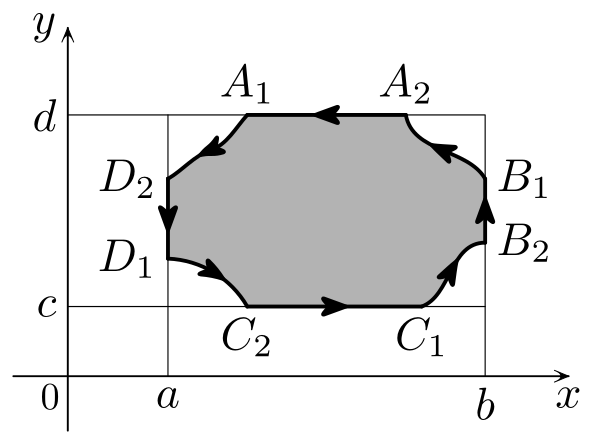
\includegraphics[width = 0.3\textwidth]{canonical.png}
        \caption{Каноническая область}
    \end{figure}

    Кривая $D_2A_1A_2B_1$ -- график функции $y = \varphi(x)$, кривая $D_1C_2C_1B_2$ -- график
    функции $y = \psi(x)$. Так как $\forall x \in (a; b) \hookrightarrow \psi(x) < \varphi(x)$ и
    $\psi, \varphi \in C[a; b]$, то $\psi(a) \leq \varphi(a)$, $\psi(b) \leq \varphi(b)$.

    Итак, точка $D_2$ расположена выше точки $D_1$ или совпадает с ней, точка $B_1$ расположена выше
    точки $B_2$ или совпадает с ней. Если $D_2$ выше $D_1$, то $D_1D_2 \subset \partial G$, если
    $B_1$ выше $B_2$, то $B_1B_2 \subset \partial G$.

    Таким образом, $\partial G$ состоит из графиков $D_2A_1A_2B_1$ и $D_1C_2C_1B_2$ непрерывных
    функций и отрезков $D_1D_2$ и $B_1B_2$, то есть $\partial G$ имеет меру нуль в $\mathbb{R}^2$
    (непрерывная на отрезке функция интегрируема на нём, а график интегрируемой на отрезке функции
     одной переменной имеем меру нуль в $\mathbb{R}^2$).

    Так как ограниченность $G$ следует из определения канонической области, а мера ноль границы
    показана выше, то $G$ измеримо по Жордану.

    Так как $P \in C^1(\overline{G})$, то $\dfrac{\partial P}{\partial y}$ ограничена и непрерывна
    на измеримом множестве $G$ $\implies$ $\dfrac{\partial P}{\partial y}$ интегрируема на $G$.
    Так как $\mu\partial G = 0$, то, применяя сведение кратного интеграла к повторному, получим:
    \begin{equation*}
        \iint\limits_{G}\frac{\partial P}{\partial y}dxdy =
        \iint\limits_{\overline{G}}\frac{\partial P}{\partial y}dxdy =
        \int\limits_{a}^{b}dx \int\limits_{\psi(x)}^{\varphi(x)} \frac{\partial P}{\partial y}dy
    \end{equation*}

    По условию $\forall x \in (a; b)$ выполняется:
    \begin{enumerate}
        \item $P \in C([\psi(x); \varphi(x)]_y);$
        \item $P \in C^1((\psi(x); \varphi(x))_y);$
        \item $\dfrac{\partial P}{\partial y}$ имеем конечные пределы в концах интервала.
    \end{enumerate}

    Тогда по теореме об односторонней производной
    $\forall x \in (a; b) \hookrightarrow P \in C^1([\psi(x); \varphi(x)]_y)$.
    Применяя формулу Ньютона-Лейбница, получим:
    \begin{equation*}
        \int\limits_{\psi(x)}^{\varphi(x)}\frac{\partial P(x, y)}{\partial y}dy =
        P(x, \varphi(x)) - P(x, \psi(x))
    \end{equation*}
    Тогда
    \begin{equation*}
        \iint\limits_{G}\frac{\partial P}{\partial y}dxdy =
        \int\limits_{a}^{b} P(x, \varphi(x))dx - \int\limits_{a}^{b} P(x, \psi(x))dx =
        \int\limits_{D_2A_1A_2B_1} P(x, y)dx - \int\limits_{D_1C_2C_1B_2} P(x, y)dx =
    \end{equation*}
    \begin{equation*}
        = -\left(\int\limits_{B_1A_2A_1D_2} P(x, y)dx + \int\limits_{D_1C_2C_1B_2} P(x, y)dx\right)
    \end{equation*}

    Так как
    \begin{equation*}
        \int\limits_{D_2D_1} P(x, y)dx = \int\limits_{B_2B_1} P(x, y)dx = 0,
    \end{equation*}
    то в сумме имеем:
    \begin{equation*}
        \iint\limits_{G}\frac{\partial P}{\partial y}dxdy = -\int\limits_{\partial G^{+}} P(x, y)dx
    \end{equation*}

    Аналогично:
    \begin{equation*}
        \iint\limits_{G}\frac{\partial Q}{\partial x}dxdy = \int\limits_{\partial G^{+}} Q(x, y)dx
    \end{equation*}

    Вычитая из второго равенства первое, получим, что требовалось.
    $\blacksquare$

    \textit{Замечание}: теорема фактически доказана для более общего случая, когда
    $P, Q \in C(\overline{G})$, $\dfrac{\partial P}{\partial y}$ и $\dfrac{\partial Q}{\partial x}$
    непрерывны и ограничены в $G$, причём существуют конечные
    \begin{equation*}
        \lim\limits_{y \to \varphi(x) - 0}\frac{\partial P}{\partial y},\
        \lim\limits_{y \to \psi(x) + 0}\frac{\partial P}{\partial y},\ x \in (a; b)
    \end{equation*}
    \begin{equation*}
        \lim\limits_{x \to \eta(y) - 0}\frac{\partial Q}{\partial x},\
        \lim\limits_{x \to \xi(y) + 0}\frac{\partial Q}{\partial x},\ y \in (c; d)
    \end{equation*}

    \textbf{Обобщение формулы Грина}: пусть
    \begin{enumerate}
        \item $G \subset \mathbb{R}^2$ -- ограниченное открытое множество;
        \item $\partial G$ состоит из конечного числа кусочно-гладких кривых;
        \item $G$ разбивается на конечное число канонических областей $G_1, \ldots, G_N$:
            \begin{enumerate}
                \item $\overline{G} = \bigcup\limits_{i = 1}^{N} \overline{G_i}$;
                \item $\forall i, j \in \{1, \ldots, N\}: i \neq j \hookrightarrow
                    G_i \cap G_j = \varnothing$;
                \item $\forall i, j \in \{1, \ldots, N\}: i \neq j \hookrightarrow
                    \overline{G_i} \cap \overline{G_j} = \partial G_i \cap \partial G_j$;
                \item $\forall i \in \{1, \ldots, N\} \hookrightarrow G_i$ -- каноническая область;
            \end{enumerate}
        \item $P, Q \in C^1(\overline{G})$;
    \end{enumerate}
    тогда
    \begin{equation*}
        \iint\limits_{G}\left(\frac{\partial Q}{\partial x} - \frac{\partial P}{\partial y}\right) dx dy =
        \int\limits_{\partial G^{+}} P(x, y)dx + Q(x, y)dy
    \end{equation*}

    $\square$
    Для каждой $G_i$, $i \in \{1, \ldots, N\}$:
    \begin{equation*}
        \iint\limits_{G_i}\left(\frac{\partial Q}{\partial x} - \frac{\partial P}{\partial y}\right) dx dy=
        \int\limits_{\partial G_{i}^{+}} P(x, y)dx + Q(x, y)dy
    \end{equation*}

    Суммируя эти равенства, получим:
    \begin{equation*}
        \iint\limits_{G}\left(\frac{\partial Q}{\partial x} - \frac{\partial P}{\partial y}\right) dx dy =
        \sum\limits_{i = 1}^{N} \int\limits_{\partial G_{i}^{+}} P(x, y)dx + Q(x, y)dy
    \end{equation*}

    В последней сумме интегралы по общим участкам границы берутся дважды в разных направлениях,
    поэтому взаимно уничтожаются. Следовательно:
    \begin{equation*}
        \sum\limits_{i = 1}^{N} \int\limits_{\partial G_{i}^{+}} P(x, y)dx + Q(x, y)dy =
        \int\limits_{\partial G^{+}} P(x, y)dx + Q(x, y)dy
    \end{equation*}
    $\blacksquare$

    \textit{Замечание}: можно показать, что формула Грина справедлива для ограниченного открытого
    множества $G$, граница которого является объединением конечного числа кусочно-гладких кривых, и
    для функций $P, Q \in C^1(\overline{G})$.

    \subsubsection{Потенциальные векторные поля}

    \textbf{Определение}: $u: \mathbb{R}^3 \to \mathbb{R}$, $u \in C^1(G)$, где
    $G \subset \mathbb{R}^3$ -- область, называется потенциалом векторного поля
    $\vec{a} = (P, Q, R)^T$ в $G$, если $\vec{a} \overset{G}{\equiv} \text{grad}\ u$; аналогичное
    определение даётся для области $G \subset \mathbb{R}^2$.

    \textbf{Определение}: векторное поле $\vec{a}$ называется потенциальным в области
    $G \subset \mathbb{R}^3$ (или $\mathbb{R}^2$), если оно имеет потенциал в этой области.

    \textbf{Определение}: пусть ориентированная кусочно-гладкая кривая в $\mathbb{R}^2$ или
    $\mathbb{R}^3$ задаётся уравнением $\vec{r} = \vec{r}(t),\ t \in [a; b]$, причём точка,
    соответствующая значению параметра $t = a$, является начальной, а соответствующая значению
    $t = b$, -- конечной; тогда кривая называется замкнутой, если её начальная и конечная точки
    совпадают.

    \textit{Замечание}: отличие от \hyperlink{complex-circuit}{определения контура в ТФКП} заключается
    в отсутствии требования простоты (могут быть самопересечения).

    \textbf{Критерий потенциальности непрерывного векторного поля}: пусть $\vec{a} \in C(G)$,
    где $G \subset \mathbb{R}^3$ (или $\mathbb{R}^2$); тогда равносильны следующие утверждения:
    \begin{enumerate}
        \item Для любой замкнутой кусочно-гладкой кривой $\Gamma \subset G$ справедливо
            \begin{equation*}
                \int\limits_{\Gamma} (\vec{a}, d\vec{r}) = 0.
            \end{equation*}
        \item $\int\limits_{\gamma} (\vec{a}, d\vec{r})$ по кусочно-гладкой кривой $\gamma \subset G$
              зависит только от начальной и конечной точек кривой, но не зависит от самой кривой.
        \item Векторное поле $\vec{a}$ потенциально.
    \end{enumerate}
    При истинности хотя бы одного из утверждений (а, значит, и всех трёх):
    \begin{equation*}
        \int\limits_{\gamma} (\vec{a}, d\vec{r}) = u(B) - u(A),
    \end{equation*}
    где $u$ -- потенциал, $A$, $B$ -- начальная и конечная точки кривой $\gamma$, соответственно.

    $\square$
    Рассмотрим случай $\mathbb{R}^3$ (случай $\mathbb{R}^2$ разбирается аналогично).

    $\boxed{1 \Rightarrow 2}$
    Рассмотрим две кусочно-гладкие кривые $\gamma_1, \gamma_2 \subset{G}$ с общим началом $A$ и
    концом $B$. Кривая $\Gamma = \gamma_1 \cup \gamma_2^{-1}$ является замкнутой кусочно-гладкой
    (сначала из точки $A$ движемся к точке $B$ по кривой $\gamma_1$, а затем из $B$ в $A$ -- по
    кривой $\gamma_2$ противоположно её ориентации). Тогда
    \begin{equation*}
        0 = \int\limits_{\Gamma} (\vec{a}, d\vec{r}) =
        \int\limits_{A \gamma_1 B} (\vec{a}, d\vec{r}) + \int\limits_{B \gamma_2 A} (\vec{a}, d\vec{r}) =
        \int\limits_{A \gamma_1 B} (\vec{a}, d\vec{r}) - \int\limits_{A \gamma_2 B} (\vec{a}, d\vec{r})
        \implies
    \end{equation*}
    \begin{equation*}
        \implies \int\limits_{A \gamma_1 B} (\vec{a}, d\vec{r}) =
        \int\limits_{A \gamma_2 B} (\vec{a}, d\vec{r})
    \end{equation*}

    $\boxed{2 \Rightarrow 3}$ Зафиксируем $A = (x_0, y_0, z_0) \in G$. Пусть $B = (x, y, z) \in G$ --
    произвольная точка. Так как $\int\limits_{\gamma} (\vec{a}, d\vec{r})$ зависит только от
    начальной и конечной точек кривой, то выражение
    \begin{equation*}
        u(x, y, z) = \int\limits_{A}^{B(x, y, z)} (\vec{a}, d\vec{r})
    \end{equation*}
    определяет однозначную функцию точки $B$, не зависящую от кусочно-гладкой кривой $\gamma$ с
    началом в $A$ и концом в $B$.

    Докажем, что $u$ -- потенциал векторного поля $\vec{a}$.

    Так как $G$ -- область, то
    \begin{equation*}
        \exists \delta > 0: U_{\delta}(B) \subset G \implies
        \exists \tau: |\tau| \leq \frac{\delta}{2},\ C = (x + \tau, y, z) \in G, [B; C] \subset G.
    \end{equation*}

    Тогда
    \begin{equation*}
        u(x + \tau, y, z) - u(x, y, z) =
        \int\limits_{A}^{C} (\vec{a}, d\vec{r}) - \int\limits_{A}^{B} (\vec{a}, d\vec{r}) =
        \int\limits_{B}^{C} (\vec{a}, d\vec{r}) =
    \end{equation*}
    \begin{equation*}
        = \int\limits_{B}^{C} P(\xi, \eta, \zeta)d\xi +
                              Q(\xi, \eta, \zeta)d\eta + R(\xi, \eta, \zeta)d\zeta\ \boxed{=}
    \end{equation*}

    Параметризуем $[B; C]$: $\xi = t$, $\eta = y$, $\zeta = z$, $t \in [x; x + \tau]$ (или
    $t \in [x; x + \tau]$, если $\tau < 0$; далее для определённости считаем, что $\tau > 0$).

    \begin{equation*}
        \boxed{=} \int\limits_{x}^{x + \tau} P(t, y, z)dt = P(\tau_0, y, z) \tau,
    \end{equation*}
    где $\tau_0 = \tau_0(\tau) \in [x; x + \tau]$ (применена теорема о среднем).

    Так как по теореме о двух милиционерах $\lim\limits_{\tau \to 0} \tau_0(\tau) = x$, а
    функция $P$ непрерывна по первому аргументу, то $\lim\limits_{\tau \to 0} P(\tau_0, y, z) =
    P(x, y, z)$. Следовательно, существует
    \begin{equation*}
        \frac{\partial u}{\partial x}(x, y, z) =
        \lim\limits_{\tau \to 0} \frac{u(x + \tau, y, z) - u(x, y, z)}{\tau} =
        \lim\limits_{\tau \to 0} P(\tau_0, y, z) = P(x, y, z).
    \end{equation*}

    В силу произвольности точки $B$ получаем: $\dfrac{\partial u}{\partial x} \overset{G}{\equiv} P$.

    Аналогично, можно показать, что $\dfrac{\partial u}{\partial y} \overset{G}{\equiv} Q$,
    $\dfrac{\partial u}{\partial z} \overset{G}{\equiv} R$.

    Значит, $u \in C^1(G)$ и является потенциалом поля $\vec{a}$.

    $\boxed{3 \Rightarrow 1}$ Пусть
    \begin{equation*}
        \frac{\partial u}{\partial x} \overset{G}{\equiv} P,\
        \frac{\partial u}{\partial y} \overset{G}{\equiv} Q,\
        \frac{\partial u}{\partial z} \overset{G}{\equiv} R.
    \end{equation*}

    Пусть также $\gamma \subset G$ -- произвольная кусочно-гладкая кривая. Параметризуем её:
    \begin{equation*}
        \gamma: \{(x, y, z) \in G: x = x(t),\ y = y(t),\ z = z(t),\ t \in [\alpha; \beta]\}
    \end{equation*}
    \begin{equation*}
        A = (x(\alpha), y(\alpha), z(\alpha))\text{ -- начало }\gamma,\
        B = (x(\beta), y(\beta), z(\beta))\text{ -- конец }\gamma.
    \end{equation*}

    Тогда
    \begin{equation*}
        \int\limits_{\gamma} Pdx + Qdy + Rdz =
        \int\limits_{\alpha}^{\beta} \left(
            \frac{\partial u}{\partial x} x'(t) +
            \frac{\partial u}{\partial y} y'(t) +
            \frac{\partial u}{\partial z} z'(t)
        \right) dt =
        \int\limits_{\alpha}^{\beta} \frac{d}{dt} \left[u(x(t), y(t), z(t))\right] dt =
    \end{equation*}
    \begin{equation*}
        = u(x(\beta), y(\beta), z(\beta)) - u(x(\alpha), y(\alpha), z(\alpha)) =
        u(B) - u(A)
    \end{equation*}

    Для замкнутой $\Gamma$: $A = B \implies \int\limits_{\gamma} Pdx + Qdy + Rdz = 0$
    $\blacksquare$

    \textbf{Следствие}: потенциал непрерывного векторного поля определяется однозначно с точностью
    до прибавления произвольной постоянной.

    $\square$
    Пусть $\vec{a} \in C(G)$ имеет в $G$ два потенциала $u$ и $v$. Тогда если $A \in G$ -- фиксированная
    точка, $B \in G$ -- произвольная точка, то
    \begin{equation*}
        \int\limits_{A}^{B} (\vec{a}, d\vec{r}) = u(B) - u(A) = v(B) - v(A) \implies
        u(B) = v(B) + u(A) - v(A)
    \end{equation*}

    Так как $A$ -- фиксированная точка, то $u(A) - v(A) = C = \text{const}$. Тогда
    $u(x, y, z) \overset{G}{\equiv} v(x, y, z) + C$.
    $\blacksquare$

    \textbf{Определение}: область $G \subset \mathbb{R}^2$ называется
    \hypertarget{simply-connected}{односвязной}, если любая замкнутая кусочно-гладкая кривая
    $\Gamma \subset G$ является границей ограниченного открытого множества $D \subset G$.

    \textbf{"Критерий"\ потенциальности непрерывно дифференцируемого векторного поля}: пусть
    $\vec{a} = (P, Q)^T \in C^1(G)$, $G \subset \mathbb{R}^2$ -- область;
    \begin{enumerate}
        \item если $\vec{a}$ потенциально в $G$, то
              $\dfrac{\partial Q}{\partial x} \overset{G}{\equiv} \dfrac{\partial P}{\partial y}$;
        \item если $G$ является односвязной и
              $\dfrac{\partial Q}{\partial x} \overset{G}{\equiv} \dfrac{\partial P}{\partial y}$,
              то $\vec{a}$ потенциально в $G$.
    \end{enumerate}

    $\square$
    1) Если поле $\vec{a}$ потенциально, то существует такая $u \in C^1(G)$, что
    \begin{equation*}
        P = \frac{\partial u}{\partial x},\ Q = \frac{\partial u}{\partial y}.
    \end{equation*}

    Так как $P, Q \in C^1(G)$, то $u \in C^2(G)$. Тогда
    \begin{equation*}
        \frac{\partial^2 u}{\partial x \partial y} \overset{G}{\equiv}
        \frac{\partial^2 u}{\partial y \partial x} \iff
        \frac{\partial Q}{\partial x} \overset{G}{\equiv} \frac{\partial P}{\partial y}.
    \end{equation*}

    2) Пусть $\dfrac{\partial Q}{\partial x} \overset{G}{\equiv} \dfrac{\partial P}{\partial y}$
    и $G$ односвязна. Пусть $\Gamma \subset G$ -- замкнутая кусочно-гладкая кривая. В силу односвязности
    $G$ кривая $\Gamma$ является границей ограниченного открытого множества $D \subset G$. По
    формуле Грина (в самой общей формулировке из замечания):
    \begin{equation*}
        \int\limits_{\Gamma} Pdx + Qdy =
        \iint\limits_{D} \left(\frac{\partial Q}{\partial x} -
                               \frac{\partial P}{\partial y}\right) dx dy = 0.
    \end{equation*}

    Так как $\Gamma$ произвольна и интеграл по ней равен 0, то поле $\vec{a}$ потенциально в $G$.
    $\blacksquare$

    \textit{Замечание}: сформулированное выше утверждение не является критерием в полной мере,
    поскольку пункт 2 вносит дополнительное ограничение на область $G$; именно поэтому слово
    \textit{Критерий} взято в кавычки.

\newpage
\subsection{\textit{БИЛЕТ 15}. Формула Остроградского-Гаусса. Соленоидальные векторные поля}

    \subsubsection{Формула Остроградского-Гаусса}

    \textbf{Определение}: область $G \subset \mathbb{R}^3$ называется канонической, если
    \begin{equation*}
        G = \{(x, y, z): (x, y) \in G_1,\ \psi(x, y) < z < \varphi(x, y)\} \wedge
    \end{equation*}
    \begin{equation*}
        G = \{(x, y, z): (y, z) \in G_2,\ \xi(y, z) < x < \eta(y, z)\} \wedge
    \end{equation*}
    \begin{equation*}
        G = \{(x, y, z): (z, x) \in G_3,\ \alpha(z, x) < y < \beta(z, x)\},
    \end{equation*}
    где $G_1, G_2, G_3 \subset \mathbb{R}^2$ -- измеримые области, $\psi, \varphi \in C(\overline{G_1})$,
    $\xi, \eta \in C(\overline{G_2})$, $\alpha, \beta \in C(\overline{G_3})$.

    \textit{Замечание}: замыкание канонической области является простым множеством относительно всех
    трёх осей.

    \textbf{Определение (поверхностный интеграл второго рода специального вида)}: пусть $S_z$ --
    график функции $z \in C(\overline{G_{xy}})$, $G_{xy} \subset \mathbb{R}^2$ -- ограниченная
    область, $R \in C(S_z)$; тогда
    \begin{equation*}
        \iint\limits_{S_z} R(x, y, z) dx dy
    \end{equation*}
    определяется как
    \begin{equation*}
        \pm \iint\limits_{G_{xy}} R(x, y, z(x, y)) dx dy;
    \end{equation*}
    знак плюс соответствует стороне графика, нормаль к которой образует острый угол с осью $z$,
    знак минус -- второй стороне. Аналогично определяются
    \begin{equation*}
        \iint\limits_{S_y} Q(x, y, z) dz dx = \pm \iint\limits_{G_{zx}} Q(x, y(z, x), z) dz dx,\
        \iint\limits_{S_x} P(x, y, z) dy dz = \pm \iint\limits_{G_{yz}} P(x(y, z), y, z) dy dz.
    \end{equation*}

    \textbf{Формула Остроградского-Гаусса}: пусть
    \begin{enumerate}
        \item $G \subset \mathbb{R}^3$ -- каноническая область;
        \item $\vec{a} = (P, Q, R)^T \in C^1(\overline{G})$;
    \end{enumerate}
    тогда
    \begin{equation*}
        \iiint\limits_{G}\text{div}\vec{a}\ dx dy dz = \iint\limits_{\partial G}(\vec{a}, d\vec{S}),
    \end{equation*}
    то есть
    \begin{equation*}
        \iiint\limits_{G}
        \left(
            \frac{\partial P}{\partial x} + \frac{\partial Q}{\partial y} + \frac{\partial R}{\partial z}
        \right)dx dy dz =
        \iint\limits_{\partial G}(P dy dz + Q dz dx + R dx dy);
    \end{equation*}
    при этом $\partial G$ ориентирована внешней нормалью.

    $\square$
    Так как $G_1$ -- измеримая область, то $\mu \partial G_1 = 0$ $\implies$ $\overline{G_1}$ --
    измеримый компакт.

    Так как $\psi, \varphi \in C(\overline{G_1})$, $\overline{G_1}$ -- измеримый компакт, то
    $\psi, \varphi$ интегрируемы на $\overline{G_1}$ $\implies$ мера графиков $\psi, \varphi$
    равна 0.

    Так как $\partial G$ состоит из графиков $\psi, \varphi$ и части цилиндрической поверхности,
    то $\mu\partial G = 0$ $\implies$ $G$ измеримо по Жордану.

    Так как $R \in C^1(\overline{G})$, то $\dfrac{\partial R}{\partial z}$ непрерывна и ограничена
    на измеримом множестве $G$ $\implies$ $\dfrac{\partial R}{\partial z}$ интегрируема на
    $G$. Так как $\mu\partial G = 0$, то, применяя сведение кратного интеграла к повторному,
    рассматривая при этом $\overline{G}$ как простое множество относительно оси $z$, получим:
    \begin{equation*}
        \iiint\limits_{G}\frac{\partial R}{\partial z} dx dy dz =
        \iiint\limits_{\overline{G}}\frac{\partial R}{\partial z} dx dy dz =
        \iint\limits_{\overline{G_1}}dx dy \int\limits_{\psi(x, y)}^{\varphi(x, y)}
        \frac{\partial R(x, y, z)}{\partial z}dz
    \end{equation*}

    По условию $\forall (x, y) \in G_1$:
    \begin{enumerate}
        \item $R \in C([\psi(x, y); \varphi(x, y)]_z)$;
        \item $R \in C^1((\psi(x, y); \varphi(x, y))_z)$;
        \item $\dfrac{\partial R}{\partial z}$ имеем конечные пределы в концах интервала.
    \end{enumerate}

    Тогда по теореме об односторонней производной
    $\forall (x, y) \in G_1 \hookrightarrow R \in C^1([\psi(x, y); \varphi(x, y)]_z)$.
    Применяя формулу Ньютона-Лейбница, получим:
    \begin{equation*}
        \int\limits_{\psi(x, y)}^{\varphi(x, y)}\frac{\partial R(x, y, z)}{\partial z}dz =
        R(x, y, \varphi(x, y)) - R(x, y, \psi(x, y))
    \end{equation*}

    Таким образом, имеем:
    \begin{equation*}
        \iiint\limits_{G}\frac{\partial R}{\partial z} dx dy dz =
        \iint\limits_{\overline{G_1}} R(x, y, \varphi(x, y)) dx dy -
        \iint\limits_{\overline{G_1}} R(x, y, \psi(x, y)) dx dy =
    \end{equation*}
    \begin{equation*}
        = \iint\limits_{\Gamma_{\varphi}} R(x, y, z) dx dy -
        \iint\limits_{\Gamma_{\psi}} R(x, y, z) dx dy,
    \end{equation*}
    где $\Gamma_{\varphi}, \Gamma_{\psi}$ -- графики функций $\varphi, \psi \in C(\overline{G_1})$,
    ориентированные нормалью, образующей острый угол с осью $z$ (верхней нормалью).

    Так как $\partial G$ ориентирована внешней нормалью, то:
    \begin{equation*}
        \iint\limits_{\partial G} R(x, y, z) dx dy =
        \iint\limits_{\Gamma_{\varphi}} R(x, y, z) dx dy -
        \iint\limits_{\Gamma_{\psi}} R(x, y, z) dx dy +
        \iint\limits_{S} R(x, y, z) dx dy,
    \end{equation*}
    где $S$ -- часть цилиндрической поверхности, входящая в $\partial G$. Для интеграла по $S$
    имеем:
    \begin{equation*}
        \vec{a} = \begin{pmatrix}
            0 \\ 0 \\ R
        \end{pmatrix}, \
        \vec{\nu} = \begin{pmatrix}
            \nu_x \\ \nu_y \\ 0
        \end{pmatrix} \implies
        (\vec{a}, \vec{\nu}) = 0 \implies \iint\limits_{S} R(x, y, z) dx dy = 0,
    \end{equation*}
    где $\vec{\nu}$ -- вектор единичной нормали к $S$. Таким образом,
    \begin{equation*}
        \iiint\limits_{G}\frac{\partial R}{\partial z} dx dy dz =
        \iint\limits_{\partial G} R(x, y, z) dx dy
    \end{equation*}

    Аналогично, рассматривая $\overline{G}$ как простое множество относительно осей $x$ и $y$,
    получим:
    \begin{equation*}
        \iiint\limits_{G}\frac{\partial P}{\partial x} dx dy dz =
        \iint\limits_{\partial G} P(x, y, z) dy dz,\
        \iiint\limits_{G}\frac{\partial Q}{\partial y} dx dy dz =
        \iint\limits_{\partial G} Q(x, y, z) dz dx.
    \end{equation*}

    Складывая три полученных равенства, придём к требуемой формуле.
    $\blacksquare$

    \textit{Замечание}: доказательство теоремы проходит для более общего случая, когда
    $P, Q, R \in C(\overline{G})$, $\dfrac{\partial P}{\partial x}, \dfrac{\partial Q}{\partial y},
    \dfrac{\partial R}{\partial z}$ непрерывны и ограничены в $G$, причём существуют конечные
    \begin{equation*}
        \lim\limits_{z \to \varphi(x, y) - 0} \frac{\partial R}{\partial z},\
        \lim\limits_{z \to \psi(x, y) + 0} \frac{\partial R}{\partial z},\ (x, y) \in \overline{G_1}
    \end{equation*}
    \begin{equation*}
        \lim\limits_{x \to \eta(y, z) - 0} \frac{\partial P}{\partial x},\
        \lim\limits_{x \to \xi(y, z) + 0} \frac{\partial P}{\partial x},\ (y, z) \in \overline{G_2}
    \end{equation*}
    \begin{equation*}
        \lim\limits_{y \to \beta(z, x) - 0} \frac{\partial Q}{\partial y},\
        \lim\limits_{y \to \alpha(z, x) + 0} \frac{\partial Q}{\partial y},\ (z, x) \in \overline{G_2}
    \end{equation*}

    \textbf{Обобщение формулы Остроградского-Гаусса}: пусть
    \begin{enumerate}
        \item $G \subset \mathbb{R}^3$ -- ограниченное открытое множество;
        \item $\partial G$ состоит из конечного числа КГП;
        \item $G$ разбивается на конечное число канонических областей $G_1, \ldots, G_N$:
            \begin{enumerate}
                \item $\overline{G} = \bigcup\limits_{i = 1}^{N} \overline{G_i}$;
                \item $\forall i, j \in \{1, \ldots, N\}: i \neq j \hookrightarrow
                      G_i \cap G_j = \varnothing$;
                \item $\forall i, j \in \{1, \ldots, N\}: i \neq j \hookrightarrow
                      \overline{G_i} \cap \overline{G_j} = \partial G_i \cap \partial G_j$;
                \item $\forall i \in \{1, \ldots, N\} \hookrightarrow G_i$ -- каноническая область;
            \end{enumerate}
        \item $\vec{a} = (P, Q, R)^T \in C^1(\overline{G})$;
    \end{enumerate}
    тогда
    \begin{equation*}
        \iiint\limits_{G}\text{div}\vec{a}\ dx dy dz = \iint\limits_{\partial G}(\vec{a}, d\vec{S}),
    \end{equation*}
    при этом $\partial G$ ориентирована внешней нормалью.

    $\square$
    Для каждой $G_i, i \in \{1, \ldots, N\}$:
    \begin{equation*}
        \iiint\limits_{G_i}\text{div}\vec{a}\ dx dy dz = \iint\limits_{\partial G_i}(\vec{a}, d\vec{S}),
    \end{equation*}
    где поверхностный интеграл берётся по внешней стороне $\partial G_i$. Суммируя эти равенства,
    получим:
    \begin{equation*}
        \iiint\limits_{G}\text{div}\vec{a}\ dx dy dz =
        \sum\limits_{i = 1}^{N} \iint\limits_{\partial G_i}(\vec{a}, d\vec{S}).
    \end{equation*}

    В последней сумме интегралы по общим участкам границ берутся дважды, внешние нормали к соседним
    $\partial G_i$ противоположно направлены. Поэтому общие слагаемые взаимно уничтожаются.
    Следовательно
    \begin{equation*}
        \sum\limits_{i = 1}^{N} \iint\limits_{\partial G_i}(\vec{a}, d\vec{S}) =
        \iint\limits_{\partial G}(\vec{a}, d\vec{S}).
    \end{equation*}
    $\blacksquare$

    \textit{Замечание}: можно показать, что формула Остроградского-Гаусса справедлива для ограниченного
    открытого множества $G$, граница которого является объединением конечного числа КГП, и для
    векторного поля $\vec{a} \in C^1(\overline{G})$.

    \subsubsection{Соленоидальные векторные поля}

    \textbf{Определение}: замкнутой КГП называется такая КГП, которая является границей некоторого
    ограниченного открытого множества в $\mathbb{R}^3$.

    \textbf{Определение}: область $G \subset \mathbb{R}^3$ называется объёмно односвязной, если
    любая замкнутая КГП $S \subset G$ является границей ограниченного открытого множества $D \subset G$.

    \textbf{Определение}: векторное поле $\vec{a}$ называется соленоидальным в области
    $G \subset \mathbb{R}^3$, если поток этого поля через любую замкнутую КГП $S \subset G$ равен 0,
    то есть
    \begin{equation*}
        \forall S \subset G,\ S\text{ -- замкнутая КГП} \hookrightarrow \iint\limits_{S} (\vec{a}, d\vec{S}) = 0.
    \end{equation*}

    Приведём без доказательства утверждение, необходимое для дальнейшего изложения.

    \textbf{Геометрический смысл дивергенции}: пусть $\vec{a} \in C^1(U_{\delta}(M_0))$,
    $M_0 \in \mathbb{R}^3$, $\delta > 0$; тогда
    \begin{equation*}
        \text{div}\vec{a}(M_0) =
        \lim\limits_{k \to \infty} \frac{1}{\mu G_k} \iint\limits_{\partial G_k} (\vec{a}, d\vec{S}),
    \end{equation*}
    где
    \begin{enumerate}
        \item $\{G_k\}$ -- последовательность канонических областей;
        \item $G_1 \supset G_2 \supset \ldots \supset G_k \supset \ldots \ni M_0$;
        \item $\vec{a} \in C^1(\overline{G_1})$;
        \item $\lim\limits_{k \to \infty} \text{diam}G_k = 0$.
    \end{enumerate}

    Доказательство можно найти в \cite{petrovich-3}.

    \textbf{"Критерий"\ соленоидальности непрерывно дифференцируемого поля}: пусть $\vec{a} \in C^1(G)$,
    $G \subset \mathbb{R}^3$ -- область;
    \begin{enumerate}
        \item если $\vec{a}$ соленоидально в $G$, то $\text{div} \vec{a} \overset{G}{\equiv} 0$;
        \item если $G$ является объёмно односвязной и $\text{div} \vec{a} \overset{G}{\equiv} 0$,
              то $\vec{a}$ соленоидально в $G$.
    \end{enumerate}

    $\square$
    1) Если $M_0 \in G$, то
    \begin{equation*}
        \text{div} \vec{a}(M_0) =
        \lim\limits_{k \to \infty} \frac{1}{\mu G_k} \iint\limits_{\partial G_k}(\vec{a}, d\vec{S}),
    \end{equation*}
    где в качестве $G_k$ можно взять последовательность окрестностей точки $M_0$, радиусы которых
    стремятся к нулю. Так как поле соленоидально, то все интегралы в последнем равенстве равны нулю
    при $G_k \subset G$ (то есть при $k \geq k_0$, $k_0 \in \mathbb{N}$) $\implies$
    $\text{div} \vec{a}(M_0) = 0$. В силу произвольности точки $M_0$ получаем
    $\text{div} \vec{a} \overset{G}{\equiv} 0$.

    2) Пусть $\text{div} \vec{a} \overset{G}{\equiv} 0$ и $G$ объёмно односвязна. Пусть $S \subset G$ --
    замкнутая КГП. В силу объёмной односвязности $G$ КГП $S$ является границей ограниченного
    открытого множества $D \subset G$. По формуле Остроградского-Гаусса (в самой общей формулировке
    из замечания):
    \begin{equation*}
        \iint\limits_{S} (\vec{a}, d\vec{S}) = \iiint\limits_{D} \text{div} \vec{a} dx dy dz = 0.
    \end{equation*}

    Так как $S$ произвольная и интеграл по ней равен 0, то поле $\vec{a}$ соленоидально в $G$.
    $\blacksquare$

    \textit{Замечание}: сформулированное выше утверждение не является критерием в полной мере,
    поскольку пункт 2 вносит дополнительное ограничение на область $G$; именно поэтому слово
    \textit{Критерий} взято в кавычки.

\newpage
\subsection{\textit{БИЛЕТ 16}. Формула Стокса}

    \textbf{Определение}: пусть $S$ -- ПГП, заданная отображением $F: \overline{G} \to \mathbb{R}_{xyz}^3$,
    где $G \subset \mathbb{R}_{uv}^2$ -- ограниченная область; тогда $\delta S = F(\partial G)$
    называется краем, а $S \setminus \delta S$ -- внутренней областью $S$.

    \textbf{Определение}: ориентация кусочно-гладкого края ПГП $S$ называется согласованной с
    ориентацией $S$, если из конца вектора единичной нормали $\vec{\nu}$, заданного ориентацией $S$,
    направление обхода $\delta S$ видно против часовой стрелки.

    \textbf{Формула Стокса}: пусть
    \begin{enumerate}
        \item $\vec{a} = (P, Q, R)^T \in C^1(G)$, $G \subset \mathbb{R}_{xyz}^3$ -- область;
        \item $S \subset G$ -- дважды непрерывно дифференцируемая ПГП, заданная уравнением
              $\vec{r} = \vec{r}(u, v)$, $(u, v) \in \overline{D}$ (то есть $\vec{r} \in C^2(\overline{D})$),
              где $D \subset \mathbb{R}_{uv}^2$ -- область, к которой применима формула Грина,
              $\partial D$ -- простая замкнутая кусочно-гладкая кривая;
        \item ориентация $S$ согласована с ориентацией её края $\Gamma$;
    \end{enumerate}
    тогда
    \begin{equation*}
        \int\limits_{\Gamma} (\vec{a}, d\vec{r}) = \iint\limits_{S} (\text{rot}\vec{a}, d\vec{S}).
    \end{equation*}

    $\square$
    Параметризуем кривую $\partial D: u = u(t),\ v = v(t),\ t \in [\alpha; \beta]$, так, что при
    возрастании $t$ от $\alpha$ к $\beta$ кривая обходится в положительном направлении в плоскости
    $\mathbb{R}_{uv}^2$.

    Так как $\partial D$ -- простая замкнутая кусочно-гладкая кривая, то $u, v \in C[\alpha; \beta]$
    и $[\alpha; \beta]$ разбивается на конечное число отрезков, на каждом из которых $u, v$
    непрерывно дифференцируемы.

    Так как $\Gamma$ -- образ $\partial D$ при отображении
    $\vec{r}(u, v) = (x(u, v), y(u, v), z(u, v))^T$, то $\Gamma$ также параметризуется
    $t \in [\alpha; \beta]$:
    \begin{equation*}
        x = x(u(t), v(t)),\ y = y(u(t), v(t)),\ z = z(u(t), v(t))
    \end{equation*}

    Так как $\vec{r}_t(t) = u'(t)\vec{r}_u + v'(t)\vec{r}_v$, где $u'(t), v'(t)$ кусочно-непрерывны
    на $[\alpha; \beta]$ и не обращаются в 0 одновременно, $\vec{r}_u, \vec{r}_v \in C^1(\overline{D})$,
    то $\Gamma$ также является кусочно-гладкой кривой, причём промежутки изменения $t$, на которых
    она является гладкой, совпадают с таковыми для $\gamma$. Учитывая также биективность отображения
    $\vec{r}$, получаем, что $\Gamma$ -- простая замкнутая кусочно-гладкая кривая.

    Отметим следующее. Пусть обход $\partial D$, соответствующий возрастанию параметра,
    осуществляется против часовой стрелки. Если $S$ ориентирована единичной нормалью
    $\vec{\nu}_1 = \dfrac{[\vec{r}_u, \vec{r}_v]}{|[\vec{r}_u, \vec{r}_v]|}$, то обход $\Gamma$,
    соответствующий возрастанию параметра, виден из конца $\vec{\nu}_1$ также против часовой стрелки.
    Более подробное рассмотрение приведено на стр. 116 \cite{petrovich-3}.

    Итак, поскольку $\Gamma$ -- простая замкнутая кусочно-гладкая кривая, то:
    \begin{equation*}
        \int\limits_{\Gamma} P(x, y, z)dx =
        \int\limits_{\alpha}^{\beta} P(x(u(t), v(t)), y(u(t), v(t)), z(u(t), v(t))) \cdot x'(t) dt =
    \end{equation*}
    \begin{equation*}
        = \int\limits_{\alpha}^{\beta} P(x(u(t), v(t)), y(u(t), v(t)), z(u(t), v(t))) \cdot
                                       (x_u u'(t) + x_v v'(t)) dt =
    \end{equation*}
    \begin{equation*}
        = \int\limits_{\gamma} Px_u du + P x_v dv\ \boxed{=}
    \end{equation*}

    Отметим, что при проведённых преобразованиях интегралов направление обхода кривой соответствует
    возрастанию $t$.

    Так как к области $D$ применима формула Грина, а также $Px_u, Px_v \in C^1(\overline{D})$ в силу
    того, что $\vec{r} \in C^2(\overline{D})$, $P \in C^1(G)$, то преобразуем последний интеграл,
    используя формулу Грина:
    \begin{equation*}
        \boxed{=} \iint\limits_{D} ((Px_v)_u - (Px_u)_v) du dv =
        \iint\limits_{D} (P_u x_v + P x_{vu} - P_v x_u - P x_{uv}) du dv\ \boxed{=}
    \end{equation*}

    Так как $\vec{r} \in C^2(\overline{D})$, то $x_{uv} \overset{G}{\equiv} x_{vu}$.

    \begin{equation*}
        \boxed{=} \iint\limits_{D} (P_u x_v - P_v x_u) du dv =
        \iint\limits_{D} ((P_x x_u + P_y y_u + P_z z_u) x_v - (P_x x_v + P_y y_v + P_z z_v) x_u) du dv =
    \end{equation*}
    \begin{equation*}
        = \iint\limits_{D} (P_z (z_u x_v - z_v x_u) - P_y (x_u y_v - x_v y_u)) du dv =
        \iint\limits_{D} \left(P_z \frac{\partial (z, x)}{\partial (u, v)} -
                               P_y \frac{\partial (x, y)}{\partial (u, v)}\right) du dv =
    \end{equation*}
    \begin{equation*}
        = \iint\limits_{S} P_z dz dx - P_y dx dy
    \end{equation*}

    Аналогично можно получить:
    \begin{equation*}
        \int\limits_{\Gamma} Q(x, y, z)dy = \iint\limits_{S} Q_x dx dy - Q_z dy dz
    \end{equation*}
    \begin{equation*}
        \int\limits_{\Gamma} R(x, y, z)dy = \iint\limits_{S} R_y dy dz - R_x dz dx
    \end{equation*}

    Складывая три полученных равенства, имеем:
    \begin{equation*}
        \int\limits_{\Gamma}(Pdx + Qdy + Rdz) =
        \iint\limits_{S} ((R_y - Q_z) dy dz + (P_z - R_x) dz dx + (Q_x - P_y) dx dy),
    \end{equation*}
    то есть
    \begin{equation*}
        \int\limits_{\Gamma} (\vec{a}, d\vec{r}) = \iint\limits_{S} (\text{rot}\vec{a}, d\vec{S}).
    \end{equation*}
    $\blacksquare$

    \textbf{Определение}: пусть $S = \bigcup\limits_{i = 1}^{N} S_i$ -- КГП, где $S_i$,
    $i \in \{1, \ldots, N\}$, -- ориентированные ПГП, имеющие общие точки разве что по своих краям
    $\Gamma_i$, причём ориентация каждой $S_i$, заданная вектором единичной нормали $\vec{\nu}^{(i)}$,
    согласована с ориентацией края $\Gamma_i$;
    \begin{enumerate}
        \item Если это можно осуществить так, чтобы на всех имеющихся общих участках краёв
              $\Gamma_i$, $\Gamma_j$, $i \neq j$, ориентации $\Gamma_i$ и $\Gamma_j$ были
              противоположны, то $S$ называется ориентируемой КГП, и её ориентация задаётся выбором
              вектора единичной нормали $\vec{\nu} = \vec{\nu}^{(i)}, (x, y, z) \in S_i$.
        \item Краем $S$ называется объединение краёв $\Gamma_i$ всех $S_i$, из которых убраны общие
              участки соседних $\Gamma_i$.
        \item Ориентация края $S$, порождённая ориентацией вошедших в него участков $\Gamma_i$,
              называется согласованной с ориентацией $S$.
    \end{enumerate}

    \textbf{Обобщение формулы Стокса}: пусть
    \begin{enumerate}
        \item $\vec{a} = (P, Q, R)^T \in C^1(G)$, $G \subset \mathbb{R}_{xyz}^3$ -- область;
        \item $S \subset G$ -- ориентируемая КГП, состоящая из ПГП $S_i$, задаваемых уравнениями
              $\vec{r}_i = \vec{r}_i(u, v)$, $(u, v) \in \overline{D_i}$, $i \in \{1, \ldots, N\}$,
              $\vec{r}_i \in C^2(\overline{G_i})$, к областям $G_i$ применима формула Грина,
              $\partial G_i$ -- замкнутые кусочно-гладкие кривые;
        \item ориентация $S$ согласована с ориентацией её края $\Gamma$;
    \end{enumerate}
    тогда
    \begin{equation*}
        \int\limits_{\Gamma} (\vec{a}, d\vec{r}) = \iint\limits_{S} (\text{rot}\vec{a}, d\vec{S}).
    \end{equation*}

    $\square$
    Если $S = \bigcup\limits_{i = 1}^{N} S_i$ -- КГП, где $S_i$, $i \in \{1, \ldots, N\}$, -- ориентированные
    ПГП, имеющие общие точки разве что по краям, то $\forall i \in \{1, \ldots, N\}$:
    \begin{equation*}
        \int\limits_{\Gamma_i} (\vec{a}, d\vec{r}) = \iint\limits_{S_i} (\text{rot}\vec{a}, d\vec{S}),
    \end{equation*}
    где ориентации $\Gamma_i$ и $S$ согласованы. По определению ориентируемой КГП согласование ориентаций
    $S_i$ можно осуществить так, чтобы на всех имеющихся общим участках краёв $\Gamma_i$, $\Gamma_j$,
    $i \neq j$, ориентации $\Gamma_i$ и $\Gamma_j$ были противоположны. Тогда суммируя последние
    равенства, получим:
    \begin{equation*}
        \sum\limits_{i = 1}^{N} \int\limits_{\Gamma_i} (\vec{a}, d\vec{r}) =
        \iint\limits_{S_i} (\text{rot}\vec{a}, d\vec{S}),
    \end{equation*}
    причём в выражении, стоящем слева, взаимно уничтожаются интегралы по противоположно ориентированным
    общим участкам краёв. Тогда если $\Gamma$ -- край $S$, то
    \begin{equation*}
        \int\limits_{\Gamma} (\vec{a}, d\vec{r}) = \iint\limits_{S} (\text{rot}\vec{a}, d\vec{S}),
    \end{equation*}
    причём ориентации $S$ и $\Gamma$ согласованы.
    $\blacksquare$

\newpage
\section{Гармонический анализ}

\subsection{\textit{БИЛЕТ 17}. Достаточные условия сходимости тригонометрического ряда Фурье в точке}

    \subsubsection{Предварительные сведения}

    \textbf{Определение}: функция $f$ называется абсолютно интегрируемой на промежутке $I \subset
    \mathbb{R}$, если интеграл (вообще говоря, несобственный с конечным числом особенностей) от
    функции $f$ по промежутку $I$ абсолютно сходится. Множество функций, абсолютно интегрируемых на
    промежутке $I$, обозначается $L_R(I)$ или $L_R^1(I)$.

    \textbf{Определение}: функция $f$ называется абсолютно интегрируемой с квадратом на промежутке
    $I \subset \mathbb{R}$, если $f \in L_R(I)$, $f^2 \in L_R(I)$. Множество функций, абсолютно
    интегрируемых с квадратом на промежутке $I$, обозначается $L^2_R(I)$.

    \textbf{Лемма Римана об осцилляции}: если $f \in L_R(I)$, где $I$ -- произвольный промежуток в
    $\mathbb{R}$, то
    \begin{equation*}
        \lim\limits_{t \to \infty} \int\limits_{I} f(x)\cos{(tx)}dx = 0,\ \
        \lim\limits_{t \to \infty} \int\limits_{I} f(x)\sin{(tx)}dx = 0
    \end{equation*}

    \textbf{Утверждение 1}: пусть $f \in L_R[-a; a]$, $a > 0$; тогда
    \begin{enumerate}
        \item Если $\forall x \in [-a; a] \hookrightarrow f(-x) = f(x)$, то
              $\int\limits_{-a}^{a} f(x)dx = 2 \int\limits_{0}^{a} f(x)dx$;
        \item Если $\forall x \in [-a; a] \hookrightarrow f(-x) = -f(x)$, то
              $\int\limits_{-a}^{a} f(x)dx = 0$.
    \end{enumerate}

    \textbf{Утверждение 2}: пусть $f \in L_R[0; T]$, $T > 0$, и имеет период $T$, (то есть
    $D(f) = \mathbb{R}$, $\forall x \in D(f) \hookrightarrow f(x + T) = f(x)$); тогда $f$ абсолютно
    интегрируема на любом конечном отрезке и
    \begin{equation*}
        \forall a \in \mathbb{R} \hookrightarrow \int\limits_{a}^{a + T} f(x)dx = \int\limits_{0}^{T} f(x)dx
    \end{equation*}

    Доказательства этих утверждений можно найти в \cite{petrovich-3}.

    \textbf{Определение}: пусть $f \in L_R[-l; l]$. Тогда числа
    \begin{equation*}
        a_n = \frac{1}{l}\int\limits_{-l}^{l} f(x)\cos{\frac{\pi n x}{l}}dx,\ n \in \mathbb{N}_0
    \end{equation*}
    \begin{equation*}
        b_n = \frac{1}{l}\int\limits_{-l}^{l} f(x)\sin{\frac{\pi n x}{l}}dx,\ n \in \mathbb{N}
    \end{equation*}
    называются коэффициентами Фурье функции $f$, а функциональный ряд
    \begin{equation*}
        \frac{a_0}{2} + \sum\limits_{n = 1}^{+\infty} \left(a_n \cos{\frac{\pi nx}{l}} +
                                                            b_n \sin{\frac{\pi nx}{l}}\right)
    \end{equation*}
    называется рядом Фурье функции $f$.

    \textit{Замечание 1}: интегралы, входящие в выражение для коэффициентов Фурье, абсолютно сходятся
    $\forall f \in L_R[-l; l]$ по признаку сравнения сходимости, так как
    \begin{equation*}
        \left|f(x)\cos{\frac{\pi nx}{l}}\right| \leq |f(x)|,\ \
        \left|f(x)\sin{\frac{\pi nx}{l}}\right| \leq |f(x)|.
    \end{equation*}

    \textit{Замечание 2}: из леммы Римана об осцилляции следует, что коэффициенты Фурье абсолютно
    интегрируемой функции стремятся к нулю при $n \to \infty$.

    \textit{Замечание 3}: функцию $f \in L_R[-l; l]$ можно продолжить на всю числовую прямую с
    периодом $2l$ (изменив, если нужно, значение $f$ в одном из концов отрезка $[-l; l]$); из
    утверждения 2 следует, что полученная периодическая функция абсолютно интегрируема на любом
    отрезке длиной $2l$, и значения интегралов в формулах для коэффициентов Фурье не изменятся,
    если интеграл рассматривать по любому отрезку длины $2l$; поэтому можно говорить о ряде
    Фурье $2l$-периодичной функции $f \in L_R[a; a + 2l]$, $a \in \mathbb{R}$.

    \subsubsection{Удобный вид частичной суммы ряда Фурье}

    Частичная сума ряда Фурье:
    \begin{equation*}
        S_n(f, x) = \frac{a_0}{2} + \sum\limits_{k = 1}^{n} \left(a_k \cos{\frac{\pi kx}{l}} +
                                                                  b_k \sin{\frac{\pi kx}{l}}\right)
    \end{equation*}

    Подставим выражения для коэффициентов Фурье:
    \begin{equation*}
        S_n(f, x) = \frac{1}{2l}\int\limits_{-l}^{l} f(t)dt +
        \sum\limits_{k = 1}^{n}
        \left[
            \frac{1}{l}\left(\int\limits_{-l}^{l}f(t)\cos{\frac{\pi kt}{l}}dt\right)\cos{\frac{\pi kx}{l}} +
            \frac{1}{l}\left(\int\limits_{-l}^{l}f(t)\sin{\frac{\pi kt}{l}}dt\right)\sin{\frac{\pi kx}{l}}
        \right] =
    \end{equation*}
    \begin{equation*}
        = \frac{1}{l}\int\limits_{-l}^{l} f(t)
        \left[
            \frac{1}{2} + \sum\limits_{k = 1}^{n}
            \left(
                \cos{\frac{\pi kt}{l}}\cos{\frac{\pi kx}{l}} +
                \sin{\frac{\pi kt}{l}}\sin{\frac{\pi kx}{l}}
            \right)
        \right]dt =
    \end{equation*}
    \begin{equation*}
        = \frac{1}{l}\int\limits_{-l}^{l} f(t)
        \left[
            \frac{1}{2} + \sum\limits_{k = 1}^{n}\cos{\frac{\pi k(t - x)}{l}}
        \right]dt
    \end{equation*}

    \textbf{Определение}: выражение
    \begin{equation*}
        D_n(x) = \frac{1}{2} + \sum\limits_{k = 1}^{n}\cos{kx}
    \end{equation*}
    называется ядром Дирихле.

    Можно показать, что (см. \cite{petrovich-2}):
    \begin{equation*}
        D_n(x) =
        \begin{cases}
            \frac{\sin{\left(n + \frac{1}{2}\right)x}}{2\sin{\frac{x}{2}}},\ x \neq 2 \pi k, k \in \mathbb{Z} \\
            n + \frac{1}{2},\ x = 2 \pi k, k \in \mathbb{Z}
        \end{cases}
    \end{equation*}

    Итак,
    \begin{equation*}
        S_n(f, x) = \frac{1}{l}\int\limits_{-l}^{l} f(t) D_n\left(\frac{\pi (t - x)}{l}\right) dt
    \end{equation*}

    Функция $D_n(x)$ имеет период $2\pi$, чётна и непрерывна в любой точке. Поэтому функция
    $D_n\left(\frac{\pi(t - x)}{l}\right)$ как функция переменной $t$ имеет период $2l$ и ограничена
    на $[-l; l]$. Значит, последний интеграл сходится абсолютно. По утверждению 2 (для $f$,
    периодически продолженной на $\mathbb{R}$):
    \begin{equation*}
        S_n(f, x) = \frac{1}{l}\int\limits_{x - l}^{x + l} f(t) D_n\left(\frac{\pi (t - x)}{l}\right) dt
    \end{equation*}

    Выполним замену $z = t - x$:
    \begin{equation*}
        S_n(f, x) = \frac{1}{l}\int\limits_{-l}^{l} f(x + z) D_n\left(\frac{\pi z}{l}\right)dz
    \end{equation*}

    Разобьём интеграл на два и выполним в одном из них замену $z \to -z$:
    \begin{equation*}
        S_n(f, x) = \frac{1}{l}
        \left[
            \int\limits_{-l}^{0} f(x + z) D_n\left(\frac{\pi z}{l}\right)dz +
            \int\limits_{0}^{l} f(x + z) D_n\left(\frac{\pi z}{l}\right)dz
        \right] =
    \end{equation*}
    \begin{equation*}
        = \frac{1}{l}
        \left[
            \int\limits_{0}^{l} f(x - z) D_n\left(\frac{\pi z}{l}\right)dz +
            \int\limits_{0}^{l} f(x + z) D_n\left(\frac{\pi z}{l}\right)dz
        \right]
    \end{equation*}

    Окончательно получаем:
    \begin{equation}\label{fourier-partial}
        \boxed{S_n(f, x) = \frac{1}{l}
               \int\limits_{0}^{l}[f(x + z) + f(x - z)] D_n\left(\frac{\pi z}{l}\right)dz}
    \end{equation}

    \subsubsection{Достаточные условия сходимости ряда Фурье}

    \textbf{Признак Дини}: пусть $f \in L_R[-l; l]$ и имеет период $2l$, $S_0$ -- такое число, что
    при некотором $\delta > 0$ сходится интеграл
    \begin{equation*}
        \int\limits_{0 \leftarrow}^{\delta} \frac{|f(x_0 + z) + f(x_0 - z) - 2S_0|}{z}dz
    \end{equation*}
    тогда ряд Фурье функции $f$ сходится в точке $x_0$ к числу $S_0$.

    $\square$ $f \in L_R[-l; l]$ и имеет период $2l$ $\implies$ $f$ абсолютно интегрируема на
    любом конечном отрезке по утверждению 2.

    Заметим, что:
    \begin{equation*}
        \int\limits_{-\pi}^{\pi} D_n(x)dx =
        \int\limits_{-\pi}^{\pi}\left(\frac{1}{2} + \cos{x} + \ldots + \cos{nx}\right)dx =
        \frac{1}{2} \cdot 2\pi = \pi
    \end{equation*}

    Так как $D_n(x)$ -- чётная функция, то:
    \begin{equation*}
        \int\limits_{0}^{\pi} D_n(x)dx = \frac{\pi}{2} \implies
        \int\limits_{0}^{l} D_n\left(\frac{\pi z}{l}\right)dz = \frac{l}{2} \implies
        S_0 = \frac{1}{l}\int\limits_{0}^{l} 2S_0 D_n\left(\frac{\pi z}{l}\right)dz
    \end{equation*}

    Далее, используем \eqref{fourier-partial}:
    \begin{equation*}
        S_n(f, x) - S_0 = \frac{1}{l}\int\limits_{0}^{l} \left[f(x + z) + f(x - z) - 2S_0\right]
        D_n\left(\frac{\pi z}{l}\right)dz =
    \end{equation*}
    \begin{equation}\label{fourier-partial-sum-minus-value}
        = \frac{1}{l}\int\limits_{0}^{l} \frac{f(x + z) + f(x - z) - 2S_0}{2\sin{\frac{\pi z}{2l}}}
        \sin{\left(\left(n + \frac{1}{2}\right)\frac{\pi z}{l}\right)}dz
    \end{equation}
    Заметим, что
    \begin{equation*}
        \frac{f(x + z) + f(x - z) - 2S_0}{2\sin{\frac{\pi z}{2l}}} =
        \frac{f(x + z) + f(x - z) - 2S_0}{z} \cdot \varphi(z),\
        \varphi(z) = \frac{z}{2\sin{\frac{\pi z}{2l}}}
    \end{equation*}

    Так как $\varphi \in C(0; l]$, $\lim\limits_{z \to 0} \varphi(z) = \dfrac{l}{\pi}$, то $\varphi$
    ограничена на $(0; l]$. Таким образом, по признаку сравнения сходимости:
    \begin{equation*}
        \frac{f(x_0 + z) + f(x_0 - z) - 2S_0}{z} \in L_R[0; l] \implies
        \frac{f(x_0 + z) + f(x_0 - z) - 2S_0}{2\sin{\frac{\pi z}{2l}}} \in L_R[0; l].
    \end{equation*}
    По лемме Римана об осцилляции интеграл в правой части \eqref{fourier-partial-sum-minus-value}
    стремится к нулю при $n \to \infty$. Поэтому $\lim\limits_{n \to \infty} S_n(f, x) = S_0$.
    $\blacksquare$

    \textbf{Определение}: пусть $f$ определена в некоторой $\mathring U_{\delta}(x_0)$ и
    $\exists f(x_0 + 0), f(x_0 - 0) \in \mathbb{R}$, причём
    \begin{equation*}
        \exists \alpha > 0, C > 0: \forall u \in (0; \delta) \hookrightarrow
        |f(x_0 + u) - f(x_0 + 0)| \leq C u^{\alpha} \wedge
        |f(x_0 - u) - f(x_0 - 0)| \leq C u^{\alpha};
    \end{equation*}
    тогда говорят, что функция $f$ удовлетворяет в точке $x_0$ условию Липшица (Гёльдера) порядка
    $\alpha$; множество таких функция обозначается $\text{Lip}_{\alpha}(x_0)$.

    \textit{Замечание}: при $\alpha > \beta > 0$ выполнено
    $\text{Lip}_{\alpha}(x_0) \subset \text{Lip}_{\beta}(x_0)$.

    \textbf{Признак Липшица}: пусть $f \in L_R[-l; l]$ и имеет период $2l$, причём
    $f \in \text{Lip}_{\alpha}(x_0)$, $\alpha > 0$; тогда
    \begin{equation*}
        \lim\limits_{n \to \infty} S_n(f, x) = \frac{f(x_0 + 0) + f(x_0 - 0)}{2}
    \end{equation*}

    $\square$
    Обозначим: $S_0 = \dfrac{f(x_0 + 0) + f(x_0 - 0)}{2}$.

    \begin{equation*}
        \forall z \in (0; \delta) \hookrightarrow
        \frac{|f(x_0 + z) + f(x_0 - z) - 2S_0|}{z} \leq
        \frac{|f(x_0 + z) - f(x_0 + 0)| + |f(x_0 - z) - f(x_0 - 0)|}{z} \leq
    \end{equation*}
    \begin{equation*}
        \leq \frac{C z^{\alpha} + C z^{\alpha}}{z} = \frac{2C}{z^{1 - \alpha}}
    \end{equation*}

    Далее,
    \begin{equation*}
        \alpha > 0 \implies 1 - \alpha < 1 \implies
        \int\limits_{0}^{\delta} \frac{dz}{z^{1 - \alpha}}\text{ сходится} \implies
    \end{equation*}
    \begin{equation*}
        \implies \int\limits_{0}^{\delta} \frac{|f(x_0 + z) + f(x_0 - z) - 2S_0|}{z}dz
        \text{ сходится по признаку сравнения сходимости}
    \end{equation*}
    Тогда по признаку Дини: $\lim\limits_{n \to \infty} S_n(f, x) = S_0$.
    $\blacksquare$

    \textbf{Следствие 1 из признака Липшица}: пусть $f \in L_R[-l; l]$ имеет период $2l$, причём
    $f$ непрерывна и имеет конечные односторонние производные $f'_{+}(x_0)$ и $f'_{-}(x_0)$ в точке
    $x_0$; тогда ряд Фурье $f$ сходится в точке $x_0$ к значению $f(x_0)$.

    $\square$ По определению односторонней производной:
    \begin{equation*}
        f'_{+}(x_0) = \lim\limits_{t \to +0}\frac{f(x_0 + t) - f(x_0)}{t} = A
    \end{equation*}
    Тогда, положив $\varepsilon = 1$ в определении предела, получим:
    \begin{equation*}
        \exists \delta_1 > 0: \forall t \in (0; \delta_1) \hookrightarrow
        \left|\frac{f(x_0 + t) - f(x_0)}{t} - A\right| \leq 1
    \end{equation*}
    \begin{equation*}
        \left|\frac{f(x_0 + t) - f(x_0)}{t} - A\right| \leq 1 \iff
        |f(x_0 + t) - f(x_0) - At| \leq t
    \end{equation*}
    Так как $\forall a, b \in \mathbb{R} \hookrightarrow |a - b| \geq ||a| - |b||$, то:
    \begin{equation*}
        \Big||f(x_0 + t) - f(x_0)| - |A|t\Big|\leq |f(x_0 + t) - f(x_0) - At| \leq t \implies
        -t \leq |f(x_0 + t) - f(x_0)| - |A|t \leq t \implies
    \end{equation*}
    \begin{equation*}
        \implies |f(x_0 + t) - f(x_0)| \leq (|A| + 1)t
    \end{equation*}
    Итак,
    \begin{equation*}
        \exists \delta_1 > 0: \forall t \in (0; \delta_1) \hookrightarrow
        |f(x_0 + t) - f(x_0)| \leq (|A| + 1)t
    \end{equation*}

    Аналогично из существования $f'_{-}(x_0) = B$ следует, что
    \begin{equation*}
        \exists \delta_2 > 0: \forall t \in (0; \delta_2) \hookrightarrow
        |f(x_0 - t) - f(x_0)| \leq (|B| + 1)t
    \end{equation*}

    Пусть $\delta = \min(\delta_1, \delta_2)$, $C = \max(|A| + 1, |B| + 1)$. Тогда:
    \begin{equation*}
        \forall t \in (0; \delta) \hookrightarrow |f(x_0 + t) - f(x_0)| \leq Ct \wedge
        |f(x_0 - t) - f(x_0)| \leq Ct
    \end{equation*}

    Поскольку также $f(x_0 + 0) = f(x_0 - 0) = f(x_0)$ в силу непрерывности $f$ в точке $x_0$, то
    $f \in \text{Lip}_{1}(x_0)$. Тогда по признаку Липшица:
    \begin{equation*}
        \lim\limits_{n \to \infty} S_n(f, x) = \frac{f(x_0 + 0) + f(x_0 - 0)}{2} = f(x_0)
    \end{equation*}

    $\blacksquare$

    \textbf{Определение}: говорят, что функция $f$, определённая в некоторой проколотой правой
    (левой) окрестности точки $x_0$, имеет обобщённую правую (левую) одностороннюю производную, если
    существуют конечные пределы $f(x_0 + 0)$ и $\lim\limits_{t \to +0}\dfrac{f(x_0 + t) - f(x_0 + 0)}{t}$
    (соответственно $f(x_0 - 0)$ и $\lim\limits_{t \to +0}\dfrac{f(x_0 - t) - f(x_0 - 0)}{-t}$).

    \textbf{Следствие 2 из признака Липшица}: пусть $f \in L_R[-l; l]$ имеет период $2l$, причём
    в точке $x_0$ у неё разрыв первого рода и существуют конечные обобщённые односторонние производные;
    тогда ряд Фурье $f$ сходится в точке $x_0$ к значению $\dfrac{f(x_0 + 0) + f(x_0 - 0)}{2}$.

    $\square$
    Доказательство аналогично, но без условия непрерывности $f$ в точке $x_0$.
    $\blacksquare$

\newpage
\subsection{\textit{БИЛЕТ 18}. Достаточные условия равномерной сходимости тригонометрического
            ряда Фурье в точке}

    \textbf{Определение}: функция $f$ называется кусочно непрерывно дифференцируемой на отрезке
    $[a; b]$, если этот отрезок можно разбить на конечное число отрезков, на каждом из которых
    функция $f$ (возможно, после изменения значений в концах) непрерывно дифференцируема.

    \textbf{Определение}: функция $f$ называется кусочно-гладкой на отрезке $[a; b]$, если она
    непрерывна и кусочно непрерывно дифференцируема на $[a; b]$.

    Приведём без доказательства утверждение, необходимое для дальнейшего изложения.

    \textbf{Неравенство Бесселя}: пусть $e_1, \ldots, e_n, \ldots$ -- счётная ортонормированная
    система в бесконечномерном евклидовом пространстве $L$; $x \in L$; $c_1, \ldots, c_n, \ldots$ --
    коэффициенты Фурье $x$ по данной системе; тогда ряд $\sum\limits_{n = 1}^{+\infty} c_n^2$
    сходится и $\sum\limits_{n = 1}^{+\infty} c_n^2 \leq \|x\|^2$.

    Доказательство можно найти в \cite{petrovich-3}.

    \textbf{Теорема}: пусть $f$ является кусочно-гладкой на отрезке $[-l; l]$, $l > 0$, и имеет
    период $2l$; тогда:
    \begin{enumerate}
        \item Ряд Фурье функции $f$
        \begin{equation*}
            \frac{a_0}{2} + \sum\limits_{n = 1}^{+\infty}
            \left(
                a_n \cos{\frac{\pi n x}{l}} + b_n \sin{\frac{\pi n x}{l}}
            \right)
        \end{equation*}
        сходится равномерно к $f$ на $\mathbb{R}$;
        \item Производная $f'$ имеет ряд Фурье
        \begin{equation*}
            \sum\limits_{n = 1}^{+\infty}\frac{\pi n}{l}
            \left(
                -a_n \sin{\frac{\pi n x}{l}} + b_n \cos{\frac{\pi n x}{l}}
            \right),
        \end{equation*}
        который получается формальным дифференцированием ряда Фурье функции $f$.
    \end{enumerate}

    $\square$
    Докажем сначала вторую часть теоремы.

    Пусть $f'$ имеет ряд Фурье:
    \begin{equation*}
        \frac{\alpha_0}{2} + \sum\limits_{n = 1}^{+\infty}
        \left(
            \alpha_n \cos{\frac{\pi n x}{l}} + \beta_n \sin{\frac{\pi n x}{l}}
        \right)
    \end{equation*}

    Так как $f'$ кусочно-непрерывна, то к ней применима формула Ньютона-Лейбница, причём $f$ --
    обобщённая первообразная. Поэтому в силу $2l$-периодичности функции $f$:
    \begin{equation*}
        \alpha_0 = \frac{1}{l}\int\limits_{-l}^{l} f'(x)dx = \frac{f(l) - f(-l)}{l} = 0
    \end{equation*}

    Поскольку для кусочно-гладких функций справедлива формула интегрирования по частям, имеем:
    \begin{equation*}
        \alpha_n = \frac{1}{l}\int\limits_{-l}^{l} f'(x) \cos{\frac{\pi nx}{l}}dx =
        \frac{1}{l} \cdot f(x)\cos{\frac{\pi nx}{l}}\Big|_{-l}^{l} -
            \frac{1}{l}\int\limits_{-l}^{l} f(x) \cdot \left(-\frac{\pi n}{l}\right)\sin{\frac{\pi n x}{l}}dx =
    \end{equation*}
    \begin{equation*}
        = \frac{\pi n}{l} \cdot \frac{1}{l}\int\limits_{-l}^{l} f(x) \sin{\frac{\pi n x}{l}}dx =
        \frac{\pi n}{l} b_n
    \end{equation*}

    Аналогично: $\beta_n = -\dfrac{\pi n}{l}a_n$. Вторая часть теоремы доказана. Докажем первую часть.

    Так как $f'$ кусочно-непрерывна на $[-l; l]$, то $f' \in R[-l; l] \implies f' \in L_R^2[-l; l]$.

    Далее:
    \begin{equation*}
        \sum\limits_{k = 1}^{n} |a_k| = \frac{l}{\pi} \sum\limits_{k = 1}^{n} |\beta_k|\frac{1}{k} \leq
        \frac{l}{\pi} \sqrt{\sum\limits_{k = 1}^{n} \beta_k^2} \sqrt{\sum\limits_{k = 1}^{n} \frac{1}{k^2}}
    \end{equation*}
    Последнее неравенство -- неравенство Коши-Буняковского. Так как $f' \in L_R^2[-l; l]$, то к
    коэффициентам Фурье функции $f'$ применимо неравенство Бесселя, откуда следует, что ряд
    $\sum\limits_{k = 1}^{+\infty} \beta_k^2$ сходится. Ряд $\sum\limits_{k = 1}^{+\infty} \dfrac{1}{k^2}$
    также сходится.

    Таким образом:
    \begin{equation*}
        \sum\limits_{k = 1}^{n} |a_k| \leq \frac{l}{\pi} \sqrt{\sum\limits_{k = 1}^{+\infty} \beta_k^2}
        \sqrt{\sum\limits_{k = 1}^{+\infty} \frac{1}{k^2}} = C
    \end{equation*}

    Итак, ряд $\sum\limits_{n = 1}^{+\infty} |a_n|$ с неотрицательными членами имеет ограниченные
    частичные суммы $\implies$ он сходится. Аналогично сходится ряд $\sum\limits_{n = 1}^{+\infty} |b_n|$.

    Так как
    \begin{equation*}
        \forall x \in \mathbb{R} \hookrightarrow
        \left|a_n \cos{\frac{\pi nx}{l}} + b_n \sin{\frac{\pi nx}{l}}\right| \leq
        |a_n| + |b_n|,
    \end{equation*}
    то по признаку Вейерштрасса ряд Фурье $f$ сходится равномерно на $\mathbb{R}$. По следствию 1 из
    признака Липшица в каждой точке он сходится к значению $f$ в этой точке.
    $\blacksquare$

    \textbf{Теорема}: пусть $f$ является кусочно-непрерывной на отрезке $[-l; l]$, $l > 0$, имеет
    период $2l$ и имеет ряд Фурье:
    \begin{equation*}
        \frac{a_0}{2} + \sum\limits_{n = 1}^{+\infty}
        \left(
            a_n \cos{\frac{\pi nx}{l}} + b_n \sin{\frac{\pi nx}{l}}
        \right)
    \end{equation*}
    тогда первообразная $F(x) = \int\limits_{x_0}^{x} f(t)dt$, где $x_0 \in \mathbb{R}$ -- произвольная
    точка, является кусочно-гладкой функцией на $[-l; l]$, а функция $\Phi(x) = F(x) - \dfrac{a_0 x}{2}$
    ещё и периодической с периодом $2l$; при этом $\Phi(x)$ является суммой равномерно сходящегося
    на $\mathbb{R}$ своего ряда Фурье:
    \begin{equation*}
        \Phi(x) = \frac{C}{2} + \sum\limits_{n = 1}^{+\infty} \frac{l}{\pi n}
        \left(
            a_n \sin{\frac{\pi nx}{l}} - b_n \cos{\frac{\pi nx}{l}}
        \right),
    \end{equation*}
    где $C = \dfrac{1}{l}\int\limits_{-l}^{l} \Phi(x)dx$ (последний ряд получается формальным
    интегрированием ряда Фурье функции $f$ без свободного члена).

    $\square$
    Функция $\Phi(x) = F(x) - \dfrac{a_0 x}{2}$ является кусочно-гладкой на $[-l; l]$, так как
    имеет кусочно-непрерывную производную $f(x) - \dfrac{a_0}{2}$. Также:
    \begin{equation*}
        \Phi(x + 2l) - \Phi(x) = F(x + 2l) - F(x) - \frac{a_0(x + 2l)}{2} + \frac{a_0 x}{2} =
        \int\limits_{x}^{x + 2l} f(t)dt - a_0 l = \int\limits_{-l}^{l} f(t)dt - a_0 l = 0
    \end{equation*}
    (предпоследнее равенство обусловлено $2l$-периодичностью функции $f$).

    Итак, показано, что $\Phi$ имеет период $2l$ и является кусочно-гладкой. Тогда по предыдущей
    теореме:
    \begin{equation*}
        \frac{C}{2} + \sum\limits_{n = 1}^{+\infty}
        \left(
            A_n \cos{\frac{\pi nx}{l}} + B_n \sin{\frac{\pi nx}{l}}
        \right)
        \overset{\mathbb{R}}{\rightrightarrows} \Phi(x),
    \end{equation*}
    причём этот ряд можно почленно дифференцировать. Значит:
    \begin{enumerate}
        \item $C = \dfrac{1}{l}\int\limits_{-l}^{l}\Phi(x)dx$;
        \item Функция $\Phi'(x) = f(x) - \dfrac{a_0}{2}$ имеем ряд Фурье
        \begin{equation*}
            \sum\limits_{n = 1}^{+\infty} \frac{\pi n}{l}
            \left(
                -A_n \sin{\frac{\pi nx}{l}} + B_n \cos{\frac{\pi nx}{l}}
            \right)
        \end{equation*}
    \end{enumerate}
    Таким образом, $a_n = \dfrac{\pi n}{l}B_n$, $b_n = -\dfrac{\pi n}{l}A_n$. Окончательно,
    $A_n = -\dfrac{l}{\pi n}b_n$, $B_n = \dfrac{l}{\pi n}a_n$.
    $\blacksquare$

\newpage
\subsection{\textit{БИЛЕТ 19}. Непрерывность преобразования Фурье абсолютно интегрируемой функции.
            Преобразование Фурье производной и производная преобразования Фурье}

    \subsubsection{Интеграл Фурье}

    Пусть $f \in L_R(\mathbb{R})$. Тогда из признака сравнения сходимости несобственных интегралов
    следует, что $\forall y \in \mathbb{R}$ сходятся абсолютно интегралы:
    \begin{equation*}
        a(y) = \frac{1}{\pi}\int\limits_{-\infty}^{+\infty} f(t)\cos{(ty)}dt
    \end{equation*}
    \begin{equation*}
        b(y) = \frac{1}{\pi}\int\limits_{-\infty}^{+\infty} f(t)\sin{(ty)}dt
    \end{equation*}

    \textit{Замечание 1}: из леммы Римана об осцилляции следует, что $\lim\limits_{y \to \infty} a(y) =
    \lim\limits_{y \to \infty} b(y) = 0$.

    \textit{Замечание 2}: $a(y)$ -- чётная функция, $b(y)$ -- нечётная функция.

    \hypertarget{FT-continuity}{\textbf{Лемма 1}}: если $f \in L_R(\mathbb{R})$, то функции $a(y)$,
    $b(y)$, определённые выше, равномерно непрерывны на $\mathbb{R}$.

    $\square$
    \begin{equation*}
        \forall y_1, y_2 \in \mathbb{R} \hookrightarrow
        |a(y_2) - a(y_1)| =
        \frac{1}{\pi}\left|\int\limits_{-\infty}^{+\infty} f(t)[\cos{(ty_2)} - \cos{(ty_1)}]dt\right| \leq
    \end{equation*}
    \begin{equation*}
        \leq \frac{2}{\pi}\int\limits_{-\infty}^{+\infty}
            |f(t)|\left|\sin{\frac{t(y_1 - y_2)}{2}}\sin{\frac{t(y_1 + y_2)}{2}}\right|dt =
        \frac{2}{\pi}\int\limits_{-\infty}^{-A} (\ldots)dt +
        \frac{2}{\pi}\int\limits_{-A}^{A} (\ldots)dt +
        \frac{2}{\pi}\int\limits_{A}^{+\infty} (\ldots)dt \leq
    \end{equation*}
    \begin{equation*}
        \leq \int\limits_{-\infty}^{-A} (\ldots)dt + 2\int\limits_{-A}^{A} (\ldots)dt +
        \int\limits_{A}^{+\infty} (\ldots)dt\ \boxed{\leq}
    \end{equation*}

    Здесь $A > 0$, символ $(\ldots)$ использован для избежания громоздкости формул и представляет
    собой функцию, стоящую под последним интегралом, не использующим $(\ldots)$. Далее, в первом
    и третьем интегралах произведение синусов ограничим по модулю единицей, а во втором
    интеграле синус суммы -- единицей, а синус разности -- модулем аргумента
    ($\forall x \in \mathbb{R} \hookrightarrow |\sin{x}| \leq |x|$):
    \begin{equation*}
        \boxed{\leq} \int\limits_{-\infty}^{-A} |f(t)|dt +
        |y_2 - y_1| \cdot \int\limits_{-A}^{A} |tf(t)| dt +
        \int\limits_{A}^{+\infty} |f(t)|dt
    \end{equation*}

    Зафиксируем $\varepsilon > 0$. Так как $\int\limits_{-\infty}^{+\infty}|f(t)|dt$ сходится, то
    можно выбрать $A = A(\varepsilon)$ так, что:
    \begin{equation*}
        \int\limits_{-\infty}^{-A} |f(t)|dt < \frac{\varepsilon}{3},\ \
        \int\limits_{A}^{+\infty} |f(t)|dt < \frac{\varepsilon}{3}
    \end{equation*}

    Далее, пусть
    \begin{equation*}
        M(\varepsilon) =
        \begin{cases}
            \int\limits_{-A(\varepsilon)}^{A(\varepsilon)}|tf(t)|dt,\text{ если этот интеграл больше 0} \\
            1,\text{ в противном случае}
        \end{cases},\ \
        \delta(\varepsilon) = \frac{\varepsilon}{3M(\varepsilon)}.
    \end{equation*}

    Тогда:
    \begin{equation*}
        \forall y_1, y_2 \in \mathbb{R}: |y_2 - y_1| < \delta(\varepsilon) \hookrightarrow
        |a(y_2) - a(y_1)| < \frac{2\varepsilon}{3} + \delta(\varepsilon) \cdot M(\varepsilon) = \varepsilon
    \end{equation*}

    Итак,
    \begin{equation*}
        \forall \varepsilon > 0 \hookrightarrow \exists \delta(\varepsilon) > 0:
        \forall y_1, y_2 \in \mathbb{R}: |y_2 - y_1| < \delta \hookrightarrow |a(y_2) - a(y_1)| < \varepsilon,
    \end{equation*}
    то есть $a(y)$ равномерно непрерывна на $\mathbb{R}$. Доказательство для функции $b(y)$ проводится
    аналогично.
    $\blacksquare$

    \textbf{Определение}: пусть $f \in L_R(\mathbb{R})$, функции $a(y)$, $b(y)$ определены выше,
    тогда интеграл
    \begin{equation*}
        \int\limits_{0}^{+\infty}[a(y)\cos{(xy)} + b(y)\sin{(xy)}]dy,
    \end{equation*}
    зависящий от параметра $x$, называется интегралом Фурье функции $f$.

    Поскольку функции $a, b \in C(\mathbb{R})$, то, во-первых, $\forall B > 0$ существует собственный
    интеграл Римана:
    \begin{equation*}
        \Phi_B(x) = \int\limits_{0}^{B}[a(y)\cos{(xy)} + b(y)\sin{(xy)}]dy,
    \end{equation*}
    во-вторых, интеграл Фурье имеет единственную особенность $+\infty$. Таким образом, сходимость
    интеграла Фурье к функции $\Phi(x)$ означает, что
    \begin{equation*}
        \lim\limits_{B \to +\infty} \Phi_B(x) = \Phi(x).
    \end{equation*}

    Приведём формулировки некоторых достаточных условий сходимости интеграла Фурье в точке.

    \textbf{Признак Дини}: пусть $f \in L_R(\mathbb{R})$, $S_0$ -- такое число, что при некотором
    $\delta > 0$ сходится
    \begin{equation*}
        \int\limits_{0\leftarrow}^{\delta} \frac{|f(x_0 + t) + f(x_0 - t) - 2S_0|}{t}dt;
    \end{equation*}
    тогда интеграл Фурье функции $f$ сходится в точке $x_0$ к числу $S_0$.

    \textbf{Признак Липшица}: пусть $f \in L_R(\mathbb{R})$, причём $f \in \text{Lip}_{\alpha}(x_0)$,
    $\alpha > 0$; тогда интеграл Фурье функции $f$ сходится в точке $x_0$ к значению
    $\dfrac{f(x_0 + 0) + f(x_0 - 0)}{2}$.

    \textbf{Следствие 1 из признака Липшица}: пусть $f \in L_R(\mathbb{R})$, причём $f$ непрерывна
    и имеет конечные односторонние производные $f'_{+}(x_0)$ и $f'_{-}(x_0)$ в точке $x_0$; тогда
    интеграл Фурье функции $f$ сходится в точке $x_0$ к значению $f(x_0)$.

    \textbf{Следствие 2 из признака Липшица}: пусть $f \in L_R(\mathbb{R})$, причём в точке $x_0$ у
    неё разрыв первого рода и существуют конечные обобщённые односторонние производные; тогда
    интеграл Фурье функции $f$ сходится в точке $x_0$ к значению $\dfrac{f(x_0 + 0) + f(x_0 - 0)}{2}$.

    Доказательства приведённых признаков можно найти в \cite{petrovich-3}, где они доказываются для
    $f \in L'_C(\mathbb{R})$ -- подмножества $L_R(\mathbb{R})$, содержащего функции, кусочно-непрерывные
    на любом конечном отрезке.

    \subsubsection{Интеграл в смысле главного значения}

    \textbf{Определение}: пусть $f \in L_R[a; b]$ на любом конечном отрезке $[a; b]$; тогда если
    существует конечный $\lim\limits_{B \to +\infty} \int\limits_{-B}^{B} f(x)dx$, то он называется
    интегралом в смысле главного значения от функции $f$ по всей числовой прямой и обозначается
    \begin{equation*}
        (\text{v.p.})\int\limits_{-\infty}^{+\infty} f(x)dx.
    \end{equation*}

    \textit{Замечание 1}: если $\int\limits_{-\infty}^{+\infty} f(x)dx$ сходится, то существует
    $(\text{v.p.})\int\limits_{-\infty}^{+\infty} f(x)dx = \int\limits_{-\infty}^{+\infty} f(x)dx$.

    \textit{Замечание 2}: можно также определять интеграл в смысле главного значения по конечным
    промежуткам, причём особенность имеется в одной из внутренних точек или в обоих концах, однако
    для теории преобразования Фурье это излишне.

    \subsubsection{Комплексная форма интеграла Фурье}

    Пусть $f \in L_R(\mathbb{R})$, функции $a(y)$, $b(y)$ определены выше. Рассмотрим функцию
    \begin{equation*}
        c(y) = a(y) - ib(y) = \frac{1}{\pi}\int\limits_{-\infty}^{+\infty}f(t)e^{-ixy}dt.
    \end{equation*}

    В силу чётности $a(y)$ и нечётности $b(y)$ имеем
    \begin{equation*}
        c(-y) = a(y) + ib(y) = \frac{1}{\pi}\int\limits_{-\infty}^{+\infty}f(t)e^{ixy}dt.
    \end{equation*}

    Тогда:
    \begin{equation*}
        a(y) = \frac{c(y) + c(-y)}{2},\ \ b(y) = i\frac{c(y) - c(-y)}{2}.
    \end{equation*}
    \begin{equation*}
        \Phi_B(x) = \int\limits_{0}^{B} [a(y)\cos{(xy)} + b(y)\sin{(xy)}]dy =
        \int\limits_{0}^{B}
        \left[
            \frac{c(y) + c(-y)}{2}\cos{(xy)} + i\frac{c(y) - c(-y)}{2}\sin{(xy)}
        \right]dy =
    \end{equation*}
    \begin{equation*}
        = \frac{1}{2}\int\limits_{0}^{B} c(y)e^{ixy}dy + \frac{1}{2}\int\limits_{0}^{B} c(-y)e^{-ixy}dy =
        \frac{1}{2}\int\limits_{-B}^{B} c(y)e^{ixy}dy
    \end{equation*}

    Таким образом, сходимость интеграла Фурье функции $f$ в точке $x$ к значению $S_0$ означает, что
    \begin{equation*}
        \frac{1}{2}(\text{v.p.})\int\limits_{-\infty}^{+\infty} c(y)e^{ixy}dy = S_0
    \end{equation*}

    Теоремы о сходимости интеграла Фурье в точке могут быть сформулированы в терминах существования
    указанного выше интеграла в смысле главного значения. Например, следствие 1 из признака Липшица
    может быть сформулировано следующим образом:

    \textbf{Следствие 1 из признака Липшица в комплексной форме}: пусть $f \in L_R(\mathbb{R})$,
    причём $f$ непрерывна и имеет конечные односторонние производные в точке $x_0$; тогда если
    \begin{equation*}
        c(y) = \frac{1}{\pi}\int\limits_{-\infty}^{+\infty} f(x)e^{-ixy}dy,
    \end{equation*}
    то
    \begin{equation*}
        f(x_0) = \frac{1}{2}(\text{v.p.})\int\limits_{-\infty}^{+\infty} c(y)e^{ix_0y}dy.
    \end{equation*}

    \subsubsection{Преобразование Фурье}

    \textbf{Определение}: пусть $f: \mathbb{R} \to \mathbb{C}$ абсолютно интегрируема на любом
    конечном отрезке; тогда преобразованием Фурье функции $f$ называется функция
    \begin{equation*}
        \hat{f}(y) \equiv F[f](y) =
            \frac{1}{\sqrt{2\pi}}(\text{v.p.})\int\limits_{-\infty}^{+\infty} f(x)e^{-ixy}dx
    \end{equation*}
    обратным преобразованием Фурье функции $f$ называется функция
    \begin{equation*}
        \tilde{f}(y) \equiv F^{-1}[f](y) =
            \frac{1}{\sqrt{2\pi}}(\text{v.p.})\int\limits_{-\infty}^{+\infty} f(x)e^{ixy}dx
    \end{equation*}

    \textit{Замечание 1}: $\forall y \in \mathbb{R} \hookrightarrow F[f](-y) = F^{-1}[f](y)$.

    \textit{Замечание 2}: если $f \in L_R(\mathbb{R})$, то интегралы из определения существуют как
    абсолютно сходящиеся, а не только в смысле главного значения.

    \textbf{Теорема}: пусть $f \in L_R(\mathbb{R})$, $f \in C(\mathbb{R})$ и имеет в каждой точке
    конечные односторонние производные; тогда
    \begin{equation*}
        F^{-1}[F[f]] = f,\ \ F[F^{-1}[f]] = f
    \end{equation*}

    $\square$
    Первое утверждение вытекает из следствия 1 из признака Липшица в комплексной форме, поскольку
    $F[f](y) = \sqrt{\dfrac{\pi}{2}} c(y)$.

    Далее, заметим, что в $\text{(v.p.)}\int\limits_{-\infty}^{+\infty}\varphi(y)dy$ можно сделать
    замену $y \to -y$:
    \begin{equation*}
        \int\limits_{-B}^{B} \varphi(y)dy = \int\limits_{-B}^{B} \varphi(-y)dy \implies
        \lim\limits_{B \to +\infty}\int\limits_{-B}^{B} \varphi(y)dy =
        \lim\limits_{B \to +\infty}\int\limits_{-B}^{B} \varphi(-y)dy;
    \end{equation*}
    (оба интеграла существуют одновременно; в случае существования равны). Поэтому
    \begin{equation*}
        \forall x \in \mathbb{R} \hookrightarrow
        f(x) = \frac{1}{\sqrt{2\pi}}\text{(v.p.)}\int\limits_{-\infty}^{+\infty} \hat{f}(y)e^{ixy}dy =
        \frac{1}{\sqrt{2\pi}}\text{(v.p.)}\int\limits_{-\infty}^{+\infty} \hat{f}(-y)e^{-ixy}dy =
    \end{equation*}
    \begin{equation*}
        = \frac{1}{\sqrt{2\pi}}\text{(v.p.)}\int\limits_{-\infty}^{+\infty} \tilde{f}(y)e^{-ixy}dy,
    \end{equation*}
    то есть $F[F^{-1}[f]] = f$.
    $\blacksquare$

    \textbf{Непрерывность преобразования Фурье}: пусть $f: \mathbb{R} \to \mathbb{C}$,
    $f \in L_R(\mathbb{R})$; тогда $F[f](y)$ и $F^{-1}[f](y)$ равномерно непрерывны на $\mathbb{R}$
    и $\lim\limits_{y \to \infty} F[f](y) = \lim\limits_{y \to \infty} F^{-1}[f](y) = 0$.

    $\square$
    Утверждение теоремы следует из того, что этими же свойствами обладают функции $a(y)$ и $b(y)$
    (\hyperlink{FT-continuity}{Лемма 1}), являющиеся с точностью до числового множителя
    действительной и мнимой частями прямого и обратного преобразования Фурье.
    $\blacksquare$

    Приведём некоторые утверждения из теории интегралов, зависящих от параметра, необходимые в дальнейшем.

    \textbf{Теорема о дифференцировании несобственного интеграла по параметру}: пусть
    \begin{enumerate}
        \item $f, \dfrac{\partial f}{\partial\alpha} \in C(X)$,
              $X = \{(x, \alpha): a \leq x < b, A \leq \alpha \leq B,\}$,
              $b \in \mathbb{R} \cup \{+\infty\}$;
        \item $\int\limits_{a}^{\to b} \dfrac{\partial f}{\partial\alpha}(x, \alpha)dx$ сходится
              равномерно по $\alpha$ на $[A; B]$;
        \item $I(\alpha) = \int\limits_{a}^{\to b} f(x, \alpha)dx$ сходится при $\alpha = A$;
    \end{enumerate}
    тогда
    \begin{enumerate}
        \item $I(\alpha)$ сходится $\forall \alpha \in [A; B]$;
        \item $I \in C^1[A; B]$;
        \item $\forall \alpha \in [A; B] \hookrightarrow I'(\alpha) =
               \int\limits_{a}^{\to b} \dfrac{\partial f}{\partial\alpha}(x, \alpha)dx$, то есть
            \begin{equation*}
                \frac{d}{d\alpha}\left(\int\limits_{a}^{\to b} f(x, \alpha)dx\right) =
                \int\limits_{a}^{\to b} \frac{\partial f}{\partial\alpha}(x, \alpha)dx.
            \end{equation*}
    \end{enumerate}

    \textbf{Признак Вейерштрасса равномерной сходимости интеграла}: пусть
    \begin{enumerate}
        \item $\forall \alpha \in \Omega,\ \forall b': a < b' < b \hookrightarrow
              f(x, \alpha) \in R([a; b']_x)$ ($b \in \mathbb{R} \cup \{+\infty\}$);
        \item $\forall \alpha \in \Omega,\ \forall x \in [a; b) \hookrightarrow
              |f(x, \alpha)| \leq \varphi(x)$;
        \item $\int\limits_{a}^{\to b} \varphi(x)dx$ -- сходящийся несобственный интеграл с
              единственной особенностью $b$;
    \end{enumerate}
    тогда $\int\limits_{a}^{\to b} f(x, \alpha)dx$ сходится равномерно по $\alpha \in \Omega$.

    Доказательства этих утверждений можно найти в \cite{petrovich-3}.

    \textbf{Производная преобразования Фурье}: пусть $f \in C(\mathbb{R})$; $f, xf \in L_R(\mathbb{R})$;
    тогда $F[f](y) \in C^1(\mathbb{R})$, причём:
    \begin{equation*}
        \frac{d}{dy}F[f](y) = F[-ixf](y)
    \end{equation*}

    $\square$
    Дифференцируя по параметру $y$ интеграл
    \begin{equation*}
        F[f](y) = \frac{1}{\sqrt{2\pi}}\int\limits_{-\infty}^{+\infty} f(x)e^{-ixy}dx,
    \end{equation*}
    получим
    \begin{equation*}
        \frac{d}{dy}F[f](y) = \frac{1}{\sqrt{2\pi}}\int\limits_{-\infty}^{+\infty} (-ix)f(x)e^{-ixy}dx =
        F[-ixf](y).
    \end{equation*}

    Теперь обоснуем возможность дифференцирования по параметру.

    Сам интеграл сходится $\forall y \in \mathbb{R}$. Далее, $xf \in L_R(\mathbb{R})$ и $\forall
    y \in \mathbb{R} \hookrightarrow |-ixf(x)e^{-ixy}| = |xf(x)|$. Тогда по признаку Вейерштрасса
    продифференцированный интеграл сходится равномерно по $y$ на $\mathbb{R}$. Значит, теорема о
    дифференцировании несобственного интеграла, зависящего от параметра, применима для $y \in [A; B]$
    на любом конечном отрезке $[A; B]$. Таким образом, искомое равенство имеем место
    $\forall y \in \mathbb{R}$.
    $\blacksquare$

    \textbf{Следствие}: пусть $f \in C(\mathbb{R})$; $f, xf, \ldots, x^n f \in L_R(\mathbb{R})$,
    $n \in \mathbb{N}$; тогда $F[f](y) \in C^n(\mathbb{R})$, причём:
    \begin{equation*}
        \frac{d^k}{dy^k}F[f](y) = F[(-ix)^k f](y),\ k \in \{1, \ldots, n\}
    \end{equation*}

    \textbf{Преобразование Фурье производной}: пусть $f\in L_R(\mathbb{R})$ является кусочно-гладкой
    на любом конечном отрезке, $f' \in L_R(\mathbb{R})$; тогда
    \begin{equation*}
        \forall y \in \mathbb{R} \hookrightarrow F[f'](y) = iyF[f](y).
    \end{equation*}

    $\square$
    Так как $f$ является кусочно-гладкой на любом конечном отрезке, то
    \begin{equation*}
        \int\limits_{0}^{x} f'(t)dt = f(x) - f(0)
    \end{equation*}
    Из сходимости $\int\limits_{0}^{+\infty} f'(t)dt$ следует существование конечного
    $\lim\limits_{x \to +\infty} f(x) = C$. Так как $\int\limits_{0}^{+\infty} |f(x)|dx$ сходится,
    то $C = 0$. Аналогично $\lim\limits_{x \to -\infty} f(x) = 0$.

    Интегрируя по частям, получим:
    \begin{equation*}
        F[f'](y) = \frac{1}{\sqrt{2\pi}}\int\limits_{-\infty}^{+\infty} f'(x)e^{-ixy}dx =
        \frac{1}{\sqrt{2\pi}}f(x)e^{-ixy}\Big|_{-\infty}^{+\infty} +
        \frac{iy}{\sqrt{2\pi}}\int\limits_{-\infty}^{+\infty} f(x)e^{-ixy}dx = iyF[f](y)
    \end{equation*}
    $\blacksquare$

    \textbf{Следствие}: пусть $f$ такова, что $f^{(n - 1)}$, $n \in \mathbb{N}$, является
    кусочно-гладкой на любом конечном отрезке, причём
    $f, f', \ldots, f^{(n - 1)}, f^{(n)} \in L_R(\mathbb{R})$; тогда
    \begin{equation*}
        \forall y \in \mathbb{R} \hookrightarrow F[f^{(n)}](y) = (iy)^n F[f](y)
    \end{equation*}
    и $F[f](y) = o\left(\dfrac{1}{y^n}\right), y \to \infty$.

\newpage
\section{Аналитическая геометрия}

\subsection{\textit{БИЛЕТ 20}. Прямые и плоскости в пространстве. Формулы расстояния от точки до
            прямой и плоскости, между прямыми в пространстве. Углы между прямыми и плоскостями}

    \subsubsection{Параметрическое уравнение прямой}

    Прямая линия на плоскости и в пространстве полностью определяется, если на ней задана точка $M_0$
    (начальная точка) и задан ненулевой вектор $\vec{a}$, параллельный этой прямой (направляющий
    вектор).

    Пусть дана прямая $l$. Обозначим через $\vec{r}_0$ радиус-вектор точки $M_0$. Рассмотрим
    произвольную точку $M$ с радиус-вектором $\vec{r}$. Тогда
    \begin{equation*}
        M \in l \iff
        \overrightarrow{M_0M} = \vec{r} - \vec{r}_0 \parallel l \iff
        \vec{r} - \vec{r}_0 \parallel \vec{a} \iff
        \exists t \in \mathbb{R}: \vec{r} - \vec{r}_0 = t\vec{a}
    \end{equation*}
    Итак, получили:
    \begin{equation*}
        \boxed{\vec{r} = \vec{r}_0 + t\vec{a}}\text{ -- векторное параметрическое уравнение прямой}
    \end{equation*}

    Пусть в трёхмерном пространстве задан некоторый базис. Рассматриваемые векторы имеют в нём
    координаты:
    \begin{equation*}
        \vec{r} =
        \begin{pmatrix}
            x \\ y \\ z
        \end{pmatrix},\
        \vec{r}_0 =
        \begin{pmatrix}
            x_0 \\ y_0 \\ z_0
        \end{pmatrix},\
        \vec{a} =
        \begin{pmatrix}
            a_1 \\ a_2 \\ a_3
        \end{pmatrix}
    \end{equation*}
    Тогда раскладывая по базису обе части векторного параметрического уравнения, получим:
    \begin{equation*}
        \boxed{\begin{cases}
            x = x_0 + a_1 t \\
            y = y_0 + a_2 t \\
            z = z_0 + a_3 t
        \end{cases}}\text{ -- параметрическое уравнение прямой}
    \end{equation*}
    Для прямой на плоскости в системе нужно оставить лишь одно уравнение.

    \subsubsection{Прямая линия на плоскости}

    Приведём без доказательства условие коллинеарности векторов в пространстве.

    \textbf{Теорема}: пусть в некотором базисе $\vec{a} = (\alpha_1, \alpha_2, \alpha_3)^T$,
    $\vec{b} = (\beta_1, \beta_2, \beta_3)^T$; тогда
    \begin{equation*}
        \vec{a} \parallel \vec{b} \iff
        \text{det}
        \begin{pmatrix}
            \alpha_1 & \alpha_2 \\
            \beta_1  & \beta_2
        \end{pmatrix} =
        \text{det}
        \begin{pmatrix}
            \alpha_2 & \alpha_3 \\
            \beta_2  & \beta_3
        \end{pmatrix} =
        \text{det}
        \begin{pmatrix}
            \alpha_3 & \alpha_1 \\
            \beta_3  & \beta_1
        \end{pmatrix} = 0
    \end{equation*}

    Доказательство можно найти в \cite{beklemishev}.

    \textbf{Утверждение 1}: пусть в некотором базисе $\vec{a} = (\alpha_1, \alpha_2)^T$,
    $\vec{b} = (\beta_1, \beta_2)^T$; тогда
    \begin{equation*}
        \vec{a} \parallel \vec{b} \iff \text{det}
        \begin{pmatrix}
            \alpha_1 & \alpha_2 \\
            \beta_1  & \beta_2
        \end{pmatrix} = 0
    \end{equation*}

    $\square$
    Считаем, что плоскость, на которой рассматриваются данные векторы, помещена в трёхмерное
    пространство, и базис на плоскости дополнен третьим вектором до базиса в пространстве. Тогда
    в новом базисе:
    \begin{equation*}
        \vec{a} =
        \begin{pmatrix}
            \alpha_1 \\ \alpha_2 \\ 0
        \end{pmatrix},\
        \vec{b} =
        \begin{pmatrix}
            \beta_1 \\ \beta_2 \\ 0
        \end{pmatrix}
    \end{equation*}

    Далее, применяя условие коллинеарности векторов в пространстве, получаем, что требовалось.
    $\blacksquare$

    \textbf{Теорема}: в ОДСК на плоскости каждая прямая  может быть задана линейным уравнением
    \begin{equation}\label{planar-line-equation}
        \boxed{Ax + By + C = 0,\ A^2 + B^2 \neq 0};
    \end{equation}
    каждое такое уравнение в ОДСК на плоскости определяет прямую.

    $\square$
    Пусть дана прямая $l$, $M_0 \in l$, $M$ -- произвольная точка плоскости. Пусть в данной ОДСК:
    \begin{equation*}
        M(x, y),\ M_0(x_0, y_0),\ \vec{a} =
        \begin{pmatrix}
            a_1 \\ a_2
        \end{pmatrix}
    \end{equation*}

    Условие $M \in l$, как установлено выше, равносильно условию $\overrightarrow{M_0M} \parallel \vec{a}$.
    Согласно утверждению 1, это может быть записано в виде:
    \begin{equation*}
        \text{det}
        \begin{pmatrix}
            x - x_0 & y - y_0 \\
            a_1     & a_2     \\
        \end{pmatrix} = 0 \iff
        a_2 (x - x_0) - a_1 (y - y_0) = 0 \iff
        a_2 x - a_1 y + (a_1 y_0 - a_2 x_0) = 0
    \end{equation*}

    Введём обозначения: $A = a_2$, $B = -a_1$, $C = a_1 y_0 - a_2 x_0$. Тогда уравнение прямой
    примет искомый вид. Отметим, что $A^2 + B^3 = a_1^2 + a_2^2 = |\vec{a}|^2 \neq 0$.

    Пусть теперь задан произвольный линейный многочлен $Ax + By + C = 0,\ A^2 + B^2 \neq 0$. Покажем,
    что
    \begin{equation*}
        \exists M_0(x_0, y_0),\ \vec{a} = (a_1, a_2)^T: \forall x, y \in \mathbb{R} \hookrightarrow
        Ax + By + C = \text{det}
        \begin{pmatrix}
            x - x_0 & y - y_0 \\
            a_1     & a_2
        \end{pmatrix}
    \end{equation*}

    Выберем $x_0$ и $y_0$ так, чтобы $Ax_0 + By_0 + C = 0$. Например:
    \begin{equation}\label{point-on-line-coords}
        x_0 = -\frac{AC}{A^2 + B^2},\ y_0 = -\frac{BC}{A^2 + B^2}
    \end{equation}

    Тогда
    \begin{equation*}
        C = -Ax_0 - By_0 \implies Ax + By + C = A(x - x_0) + B(y - y_0)
    \end{equation*}

    Окончательно, выбором $a_1 = -B$, $a_2 = A$ получаем, что требовалось.
    $\blacksquare$

    \textbf{Следствие 1}: в ОДСК вектор с координатами $(-B, A)^T$ можно принять за направляющий
    вектор прямой, заданной уравнением \eqref{planar-line-equation}, а точку с координатами
    \eqref{point-on-line-coords} -- за начальную точку.

    \textbf{Следствие 2}: в ПДСК вектор с координатами $(A, B)^T$ перпендикулярен прямой, заданной
    уравнением \eqref{planar-line-equation}.

    \textbf{Теорема}: вектор $\vec{a} = (\alpha_1, \alpha_2)^T$ в ОДСК параллелен прямой $l$,
    заданной уравнением $Ax + By + C = 0,\ A^2 + B^2 \neq 0$ $\iff$ $A\alpha_1 + B\alpha_2 = 0$.

    $\square$
    Вектор $\vec{b} = (-B, A)^T$ является направляющим вектором прямой.

    $\boxed{\Rightarrow}$
    \begin{equation*}
        \vec{a} \parallel l \implies \vec{a} \parallel \vec{b} \implies \text{det}
        \begin{pmatrix}
            \alpha_1 & \alpha_2 \\
            -B       & A
        \end{pmatrix} = 0 \implies A \alpha_1 + B \alpha_2 = 0
    \end{equation*}

    $\boxed{\Leftarrow}$
    Пусть $A = 0$. Так как $B \neq 0$, то $\alpha_2 = 0$ $\implies$ $\vec{a} = (\alpha_1, 0)^T$,
    $\vec{b} = (-B, 0)^T$. Так как $B \neq 0$, то $\forall k \neq 0 \hookrightarrow \alpha_1 = -kB \neq 0
    \implies \vec{a} \parallel \vec{b} \implies \vec{a} \parallel l$.

    Если $B = 0$, рассмотрение аналогично.

    Пусть теперь $A \neq 0 \wedge B \neq 0$. Тогда
    \begin{equation*}
        \dfrac{\alpha_1}{-B} = \dfrac{\alpha_2}{A} = k \implies \vec{a} = (\alpha_1, \alpha_2)^T =
        (k(-B), kA)^T = k(-B, A)^T = k\vec{b} \implies \vec{a} \parallel \vec{b}.
    \end{equation*}
    $\blacksquare$

    Для прямой на плоскости можно также написать векторное уравнение:
    \begin{equation*}
        \boxed{(\vec{r} - \vec{r}_0, \vec{n}) = 0}\text{ -- векторное уравнение прямой на плоскости}
    \end{equation*}
    Вектор $\vec{n}$ -- вектор нормали, перпендикулярный направляющему вектору $\vec{a}$.

    \subsubsection{Прямая линия в пространстве}

    Рассмотрим прямую заданную параметрическим уравнением:
    \begin{equation*}
        \begin{cases}
            x = x_0 + a_1 t \\
            y = y_0 + a_2 t \\
            z = z_0 + a_3 t
        \end{cases}
    \end{equation*}

    Если некоторая координата $\vec{a}$ равна 0, то соответствующая координата точек прямой постоянна:
    $x = x_0 = \text{const}$ при $a_1 = 0$, $y = y_0 = \text{const}$ при $a_2 = 0$,
    $z = z_0 = \text{const}$ при $a_3 = 0$.

    Если лишь одна координата $\vec{a}$ равна 0, то параметр $t$ можно выразить двумя способами.
    Например, если $a_1 = 0$, то $t = \dfrac{y - y_0}{a_2}$, $t = \dfrac{z - z_0}{a_3}$. Тогда имеем:
    \begin{equation*}
        x = x_0,\ \frac{y - y_0}{a_2} = \frac{z - z_0}{a_3}
    \end{equation*}

    Если ни одна из координат $\vec{a}$ не равна 0, то параметр $t$ можно выразить тремя способами:
    \begin{equation*}
        t = \frac{x - x_0}{a_1},\ t = \frac{y - y_0}{a_2},\ t = \frac{z - z_0}{a_3},
    \end{equation*}
    Тогда:
    \begin{equation*}
        \boxed{\frac{x - x_0}{a_1} = \frac{y - y_0}{a_2} = \frac{z - z_0}{a_3}}
        \text{ -- каноническое уравнение прямой}
    \end{equation*}

    Условие $\vec{r} - \vec{r}_0 \parallel \vec{a}$ может быть также записано в виде:
    \begin{equation*}
        \boxed{[\vec{r} - \vec{r}_0, \vec{a}] = 0}\text{ -- векторное уравнение прямой в пространстве}
    \end{equation*}

    \subsubsection{Плоскость}

    Плоскость в пространстве полностью определяется, если на ней задана точка $M_0$ (начальная точка)
    и два неколлинеарных вектора $\vec{p}$ и $\vec{q}$ (направляющие векторы).

    Пусть дана плоскость $\pi$. Обозначим через $\vec{r}_0$ радиус-вектор точки $M_0$. Рассмотрим
    произвольную точку $M$ с радиус-вектором $\vec{r}$. Так как $\vec{p} \nparallel \vec{q}$,
    то $\vec{p}$ и $\vec{q}$ образуют базис на плоскости $\pi$. Тогда
    \begin{equation*}
        M \in \pi \iff
        \overrightarrow{M_0M} = \vec{r} - \vec{r}_0 \parallel \pi \iff
        \exists t_1, t_2 \in \mathbb{R}: \vec{r} - \vec{r}_0 = t_1\vec{p} + t_2\vec{q}
    \end{equation*}

    Итак, получили:
    \begin{equation*}
        \boxed{\vec{r} = \vec{r}_0 + t_1\vec{p} + t_2\vec{q}}
        \text{ -- векторное параметрическое уравнение плоскости}
    \end{equation*}

\newpage
\subsection{\textit{БИЛЕТ 21}. Кривые второго порядка, их геометрические свойства}

    TBD

\newpage
\section{Линейная алгебра}

\newpage
\subsection{\textit{БИЛЕТ 22}. Общее решение системы линейных алгебраических уравнений. Теорема
            Кронекера-Капелли}

    TBD

\newpage
\subsection{\textit{БИЛЕТ 23}. Линейное пространство, базис и размерность. Линейное отображение
            конечномерных пространств, его матрица. Ядро и образ линейного отображения}

    TBD

\newpage
\subsection{\textit{БИЛЕТ 24}. Собственные значения и собственные векторы линейных преобразований.
            Диагонализируемость линейных преобразований}

    TBD

\newpage
\subsection{\textit{БИЛЕТ 25}. Самосопряжённые преобразования линейных пространств, свойства их
            собственных значений и собственных векторов}

    TBD

\newpage
\subsection{\textit{БИЛЕТ 26}. Приведение квадратичных форм в линейном пространстве к каноническому
            виду. Положительно определённые квадратичные формы. Критерий Сильвестра}

    TBD

\newpage
\section{Дифференциальные уравнения}

\subsection{\textit{БИЛЕТ 27}. Линейные обыкновенные дифференциальные уравнения с постоянными
            коэффициентами и правой частью -- квазимногочленом}

    TBD

\newpage
\subsection{\textit{БИЛЕТ 28}. Системы линейных однородных дифференциальных уравнений с постоянными
            коэффициентами, методы их решения}

    TBD

\newpage
\subsection{\textit{БИЛЕТ 29}. Линейные обыкновенные дифференциальные уравнения с переменными
            коэффициентами. Фундаментальная система решений. Определитель Вронского. Формула
            Лиувилля-Остроградского}

    TBD

\newpage
\subsection{\textit{БИЛЕТ 30}. Простейшая задача вариационного исчисления. Необходимые условия
            локального экстремума}

    TBD

\newpage
\section{Теория вероятностей}

\subsection{\textit{БИЛЕТ 31}. Полная система событий. Формула полной вероятности. Формула Байеса.
            Независимость событий и классов событий}

    TBD

\newpage
\subsection{\textit{БИЛЕТ 32}. Математическое ожидание и дисперсия случайной величины, их свойства.
            Вычисление для нормального распределения}

    TBD

\newpage
\subsection{\textit{БИЛЕТ 33}. Неравенство Чебышёва и закон больших чисел}

    TBD

\newpage
\subsection{\textit{БИЛЕТ 34}. Центральная предельная теорема для независимых одинаково распределённых
            случайных величин с конечной дисперсией}

    TBD

\newpage
\section{ТФКП}

\subsection{\textit{БИЛЕТ 35}. Дифференцируемость функций комплексного переменного.
            Условия Коши-Римана. Интегральная теорема Коши}

    \subsubsection{Дифференцируемость функций комплексного переменного}

    \textbf{Определение}: пусть $f$ определена и ограничена в $B_{\delta_0}(z_0)$, $z_0 \in \mathbb{C}$,
    пусть также $A \in \mathbb{C}$ и в $\mathring B_{\delta_0}(z_0)$ определена $\alpha(\Delta z)$:
    $f(z_0 + \Delta z) - f(z_0) = A \Delta z + \alpha(\Delta z)|\Delta z|$, где
    $\lim\limits_{\Delta z \to 0} \alpha(\Delta z) = 0$; тогда $f$ называется дифференцируемой в
    точке $z_0$.

    \textit{Замечание}: если $f$ дифференцируема в точке $z_0$, то
    $\dfrac{f(z_0 + \Delta z) - f(z_0)}{\Delta z} = A + \alpha(\Delta z)\dfrac{|\Delta z|}{\Delta z} \to A$
    при $\Delta z \to 0$; $A$ в этом случае называется производной функции $f$ в точке $z_0$
    (обозначение: $f'(z_0) = A$).

    \textbf{Теорема}: пусть $f(z) = u(x, y) + iv(x, y)$, $z = x + iy$, определена в $B_{\delta}(z_0)$;
    тогда $f$ дифференцируема в точке $z_0 = x_0 + i y_0$ $\iff$ $u$, $v$ дифференцируемы в точке
    $(x_0, y_0)$ и
    \begin{equation*}
        \boxed{\frac{\partial u}{\partial x}(x_0, y_0) = \frac{\partial v}{\partial y}(x_0, y_0);\
        \frac{\partial u}{\partial y}(x_0, y_0) = -\frac{\partial v}{\partial x}(x_0, y_0)}\
        \text{(условия Коши-Римана)}
    \end{equation*}

    $\square$ $\boxed{\Rightarrow}$ Так как $f$ дифференцируема в точке $z_0$, то ($A = B + iC$,
    $\alpha(\Delta z) = \beta(\Delta x, \Delta y) + i\gamma(\Delta x, \Delta y)$):

    \begin{equation*}
        [u(x_0 + \Delta x, y_0 + \Delta y) - u(x_0, y_0)]
        + i[v(x_0 + \Delta x, y_0 + \Delta y) - v(x_0, y_0)] =
    \end{equation*}
    \begin{equation}\label{complex}
        = (B + iC)(\Delta x + i\Delta y) + [\beta(\Delta x, \Delta y) + i\gamma(\Delta x, \Delta y)]
        \sqrt{\Delta x^2 + \Delta y^2}
    \end{equation}

    Выписывая последнее равенство отдельно для действительной и мнимой частей, получим:

    \begin{equation}\label{Re}
        u(x_0 + \Delta x, y_0 + \Delta y) - u(x_0, y_0) = (B\Delta x - C\Delta y) +
        \beta(\Delta x, \Delta y)\sqrt{\Delta x^2 + \Delta y^2}
    \end{equation}

    \begin{equation}\label{Im}
        v(x_0 + \Delta x, y_0 + \Delta y) - v(x_0, y_0) = (C\Delta x + B\Delta y) +
        \gamma(\Delta x, \Delta y)\sqrt{\Delta x^2 + \Delta y^2}
    \end{equation}

    Из \eqref{Re} следует, что $u$ дифференцируема в точке $(x_0, y_0)$ и
    $B = \dfrac{\partial u}{\partial x}(x_0, y_0)$, $C = -\dfrac{\partial u}{\partial y}(x_0, y_0)$.

    Из \eqref{Im} следует, что $v$ дифференцируема в точке $(x_0, y_0)$ и
    $B = \dfrac{\partial v}{\partial y}(x_0, y_0)$, $C = \dfrac{\partial v}{\partial x}(x_0, y_0)$.

    Таким образом, показана справедливость условий Коши-Римана.

    $\boxed{\Leftarrow}$ Обозначим $B = \dfrac{\partial u}{\partial x}(x_0, y_0) =
    \dfrac{\partial v}{\partial y}(x_0, y_0)$, $C = \dfrac{\partial u}{\partial y}(x_0, y_0) =
    -\dfrac{\partial v}{\partial x}(x_0, y_0)$. Тогда, имея \eqref{Re} и \eqref{Im} по условию,
    записываем \eqref{complex}; при этом $f'(z) = B + iC$. $\blacksquare$

    \textbf{Определение}: $f: \mathbb{C} \to \mathbb{C}$ называется регулярной в области $G$, если:
    \begin{enumerate}
        \item $\forall z \in G \hookrightarrow f$ дифференцируема в точке $z$;
        \item $f'(z)$ непрерывна в $G$.
    \end{enumerate}

    \textbf{Определение}: $f: \mathbb{C} \to \mathbb{C}$ называется регулярной в точке $z$, если
    она регулярна в некоторой $B_{\delta}(z)$.

    \textbf{Определение}: $f: \mathbb{C} \to \mathbb{C}$ называется регулярной на множестве
    $A \subset \mathbb{C}$, если она регулярна в каждой точке $A$.

    \subsubsection{Интегральная теорема Коши}

    \textbf{Определение}: кривой $\gamma$ в $\mathbb{C}$ называется непрерывное отображение
    $\sigma: [a; b] \to \mathbb{C}$; носителем кривой называется образ отрезка $[a; b]$ при
    отображении $\sigma$, то есть $\hat{\gamma} = \sigma([a; b])$.

    \textbf{Определение}: кривая $\gamma: z = \sigma(t)$, $t \in [a; b]$, называется простой, если
    отображение $\sigma$ инъективно.

    \textbf{Определение}: кривая $\gamma: z = \sigma(t)$, $t \in [a; b]$, называется замкнутой, если
    $\sigma(a) = \sigma(b)$.

    \textbf{Определение}: кривая $\gamma: z = \sigma(t)$, $t \in [a; b]$, называется простой замкнутой
    (\hypertarget{complex-circuit}{контуром}), если она замкнута и сужение отображения $\sigma$ на
    $[a; b)$ инъективно.

    \textbf{Определение}: кривая $\gamma: z = \sigma(t)$, $t \in [a; b]$, называется гладкой, если
    $\sigma \in C^1[a; b]$ и $\forall t \in [a; b] \hookrightarrow \sigma'(t) \neq 0$.

    \textbf{Определение}: ограниченная область $E \subset \mathbb{C}$ называется элементарной, если
    $\exists \gamma: z = \sigma(t), t \in [a; b]$ -- кусочно-гладкий контур: $\partial E = \hat{\gamma}$.

    \textbf{Определение}: область $E \subset \overline{\mathbb{C}}$ называется односвязной, если
    $\forall D\text{ -- элементарной области}: \partial D \subset E \hookrightarrow (D \subset E)
    \vee (\overline{\mathbb{C}} \setminus D \subset E)$.

    \textit{Замечание}: если область $E \subset \mathbb{C}$, то определение односвязности совпадает
    с \hyperlink{simply-connected}{таковым из математического анализа}.

    \textbf{Определение}: пусть $\gamma: z = \sigma(t) = \xi(t) + i\eta(t)$, $t \in [a; b]$ --
    кусочно-гладкая кривая, пусть также $f(\sigma(t)) \in C[a; b]$; тогда:
    \begin{equation*}
        \int\limits_{\gamma} f(z)|dz| = \int\limits_{a}^{b} f(\sigma(t))|\sigma'(t)|dt
    \end{equation*}
    \begin{equation*}
        \int\limits_{\gamma} f(z)dz = \int\limits_{a}^{b} f(\sigma(t))\sigma'(t)dt
    \end{equation*}

    \textbf{Интегральная теорема Коши для односвязной области}: пусть
    \begin{enumerate}
        \item $G \subset \mathbb{C}$ -- односвязная область;
        \item $\gamma$ -- кусочно-гладкий контур: $\hat{\gamma} \subset G$;
        \item $f$ регулярна в $G$;
    \end{enumerate}
    тогда $\int\limits_{\gamma} f(z)dz = 0$.

    $\square$ Пусть $z = x + iy$, $f(z) = u(x, y) + iv(x, y)$. Тогда:

    \begin{equation*}
        \int\limits_{\gamma} f(z)dz = \int\limits_{\gamma} udx - vdy + i \int\limits_{\gamma} udy + vdx =
        I_1 + i I_2
    \end{equation*}

    Обозначим $P(x, y) = u(x, y)$, $Q(x, y) = -v(x, y)$.

    Так как $f$ регулярна в $G$, то
    $\dfrac{\partial u}{\partial y} \overset{G}{\equiv} -\dfrac{\partial v}{\partial x}$, то есть
    $\dfrac{\partial P}{\partial y} \overset{G}{\equiv} \dfrac{\partial Q}{\partial x}$.

    Так как область $G$ односвязна, то область $D$, границей которой является $\hat{\gamma}$, --
    ограниченное открытое множество. Так как $f$ регулярна в $G \supset D$, то
    $P, Q \in C^1(\overline{D})$. Таким образом, для функций $P$ и $Q$ и области $D$ справедлива
    формула Грина:

    \begin{equation*}
        0 = \iint\limits_{D} \left(\frac{\partial Q}{\partial x} - \frac{\partial P}{\partial y}\right) dx dy=
        \int\limits_{\gamma} Pdx + Qdy = I_1
    \end{equation*}

    Доказательство того, что $I_2 = 0$, проходит аналогично, но нужно воспользоваться другим
    условием Коши-Римана. Таким образом, $\int\limits_{\gamma} f(z)dz = 0$. $\blacksquare$

    \textbf{Определение}: $G \subset \overline{\mathbb{C}}$ называется областью с простой границей
    (ОСПГ), если:
    \begin{enumerate}
        \item $\partial G = \hat{\gamma}_1 \cup \ldots \cup \hat{\gamma}_n$, где $\hat{\gamma}_k$ --
              кусочно-гладкий контур, $k \in \{1, \ldots, n\}$;
        \item $\forall k, l \in \{1, \ldots, n\} : k \neq l \hookrightarrow
               \hat{\gamma}_k \cap \hat{\gamma}_l = \varnothing$;
        \item $\forall k \in \{1, \ldots, n\} \hookrightarrow \gamma_k$ положительно ориентирована
              относительно области $G$ (при обходе кривой в положительном направлении область
              остаётся слева).
    \end{enumerate}

    \textbf{Интегральная теорема Коши для ограниченной ОСПГ}: пусть
    \begin{enumerate}
        \item $G \subset \mathbb{C}$ -- ограниченная ОСПГ;
        \item $f$ регулярна в $\overline{G}$;
    \end{enumerate}
    тогда $\int\limits_{\partial G} f(z)dz = 0$.

    $\square$ Пусть $z = x + iy$, $f(z) = u(x, y) + iv(x, y)$. Тогда:

    \begin{equation*}
        \int\limits_{\partial G} f(z)dz =
        \int\limits_{\partial G} udx - vdy + i \int\limits_{\partial G} udy + vdx =
        I_1 + i I_2
    \end{equation*}

    Обозначим $P(x, y) = u(x, y)$, $Q(x, y) = -v(x, y)$.

    Так как $f$ регулярна в $\overline{G}$, то $u, v \in C^1(\overline{G})$ и
    $\dfrac{\partial u}{\partial y} \overset{G}{\equiv} -\dfrac{\partial v}{\partial x}$, то есть
    $\dfrac{\partial P}{\partial y} \overset{G}{\equiv} \dfrac{\partial Q}{\partial x}$. Таким
    образом, для функций $P$ и $Q$ и области $G$ справедлива формула Грина:

    \begin{equation*}
        0 = \iint\limits_{G} \left(\frac{\partial Q}{\partial x} - \frac{\partial P}{\partial y}\right) dx dy =
        \int\limits_{\partial G} Pdx + Qdy = I_1
    \end{equation*}

    Доказательство того, что $I_2 = 0$, проходит аналогично, но нужно воспользоваться другим
    условием Коши-Римана. Таким образом, $\int\limits_{\partial G} f(z)dz = 0$. $\blacksquare$

\newpage
\subsection{\textit{БИЛЕТ 36}. Интегральная формула Коши. Разложение функции, регулярной в окрестности
            точки, в ряд Тейлора}

    \subsubsection{Интегральная формула Коши}

    \textbf{Теорема (интегральная формула Коши)}: пусть
    \begin{enumerate}
        \item $G \subset \mathbb{C}$ -- ограниченная ОСПГ;
        \item $f$ регулярна в $\overline{G}$;
        \item $z_0 \in G$.
    \end{enumerate}
    Тогда
    \begin{equation*}
        \boxed{f(z_0) = \frac{1}{2\pi i}\int\limits_{\partial G}\frac{f(z)}{z - z_0}dz}
    \end{equation*}

    $\square$ Зафиксируем $\varepsilon > 0$. Докажем, что
    \begin{equation*}
        \left|\int\limits_{\partial G}\frac{f(z)}{z - z_0}dz - 2\pi i f(z_0)\right| < 2 \pi\varepsilon.
    \end{equation*}

    $f$ регулярна в $\overline{G}$ $\implies$ $f$ непрерывна в точке $z_0$ $\implies$
    $\exists \delta > 0: \forall z \in \overline{B_{\delta}(z_0)} \subset G \hookrightarrow
    |f(z) - f(z_0)| < \varepsilon$.

    Пусть $\gamma = \{z \in \mathbb{C} : |z - z_0| = \delta\}$, проходимая по часовой стрелке, то есть
    $\hat{\gamma} = \partial\overline{B_{\delta}(z_0)}$. Тогда
    $\hat{\gamma} \cap \partial G = \varnothing$ в силу того, что
    $\overline{B_{\delta}(z_0)} \subset G$. Значит, $D = G \setminus \overline{B_{\delta}(z_0)}$ --
    тоже ограниченная ОСПГ.

    $f$ регулярна в $\overline{G} \implies f$ регулярна в $\overline{D}$; $\dfrac{1}{z - z_0}$
    регулярна в $\overline{D} \implies \dfrac{f(z)}{z - z_0}$ регулярна в $\overline{D}$.

    Таким образом, по интегральной теореме Коши для ограниченной ОСПГ:
    \begin{equation*}
        \int\limits_{\partial D}\frac{f(z)}{z - z_0}dz = 0
    \end{equation*}

    Так как $\partial D = \partial G \cup \hat{\gamma}$, то:
    \begin{equation*}
        0 = \int\limits_{\partial G}\frac{f(z)}{z - z_0}dz + \int\limits_{\gamma}\frac{f(z)}{z - z_0}dz
        \implies \int\limits_{\partial G}\frac{f(z)}{z - z_0}dz = -\int\limits_{\gamma}\frac{f(z)}{z - z_0}dz
    \end{equation*}

    Так как $\gamma$ обходится по часовой стрелке, то:
    \begin{equation*}
        \int\limits_{\gamma}\frac{dz}{z - z_0} = -2\pi i \implies
        -2\pi i f(z_0) = \int\limits_{\gamma}\frac{f(z_0)}{z - z_0}dz
    \end{equation*}

    Таким образом:
    \begin{equation*}
        \left|\int\limits_{\partial G}\frac{f(z)}{z - z_0}dz - 2\pi i f(z_0)\right| =
        \left|-\int\limits_{\gamma}\frac{f(z)}{z - z_0}dz + \int\limits_{\gamma}\frac{f(z_0)}{z - z_0}dz\right| =
        \left|\int\limits_{\gamma}\frac{f(z) - f(z_0)}{z - z_0}dz\right| \leq
    \end{equation*}
    \begin{equation*}
        \leq \max\limits_{z \in \hat{\gamma}}\left|\frac{f(z) - f(z_0)}{z - z_0}\right| \cdot |\gamma| =
        \frac{1}{\delta} \cdot \max\limits_{z \in \hat{\gamma}} |f(z) - f(z_0)| \cdot 2\pi\delta =
        2\pi\max\limits_{z \in \hat{\gamma}} |f(z) - f(z_0)| < 2\pi\varepsilon
    \end{equation*}

    Так как $\varepsilon > 0$ произвольно, то:
    \begin{equation*}
        \left|\int\limits_{\partial G}\frac{f(z)}{z - z_0}dz - 2\pi i f(z_0)\right| = 0 \implies
        f(z_0) = \frac{1}{2\pi i}\int\limits_{\partial G}\frac{f(z)}{z - z_0}dz
    \end{equation*}

    $\blacksquare$

    \subsubsection{Разложение функции, регулярной в окрестности точки, в ряд Тейлора}

    \textbf{Теорема Абеля}: если $\sum\limits_{n = 0}^{+\infty} c_n (z - z_0)^n$ сходится в точке
    $z_1 \neq z_0$, то он сходится абсолютно в любой точке $z: |z - z_0| < |z_1 - z_0|$, и
    $\forall r: 0 < r < |z_1 - z_0| \hookrightarrow$ ряд сходится равномерно в $\overline{B_r(z_0)}$.

    \textbf{Теорема о дифференцировании степенного ряда}: пусть $R_{\textbf{сх}} > 0$ и ряд
    $\sum\limits_{n = 0}^{+\infty} c_n (z - z_0)^n$ сходится в
    $K = \{z \in \mathbb{C}: |z - z_0| < R_{\textbf{сх}}\}$ к $S(z)$; тогда
    \begin{enumerate}
        \item ряд $\sum\limits_{n = 1}^{+\infty} n c_n (z - z_0)^{n - 1}$ имеет тот же радиус
              сходимости и сходится к $\hat{S}(z)$ в $K$;
        \item $\forall z \in K \hookrightarrow S'(z) = \hat{S}(z)$.
    \end{enumerate}

    Доказательство этих двух теорем можно найти в \cite{bunakov}.

    \textbf{Определение}: пусть $\gamma: z = \sigma(t)$, $t \in [a; b]$, -- кусочно-гладкая кривая,
    $f(\sigma(t)) \in C[a; b]$, пусть также $z \not\in \hat{\gamma}$; тогда
    \begin{equation*}
        F(z) = \frac{1}{2\pi i}\int\limits_{\gamma} \frac{f(w)}{w - z}dw
    \end{equation*}
    называется интегралом (типа) Коши.

    \textbf{Теорема}: пусть $\gamma$ -- кусочно-гладкая кривая, $z_0 \not\in \hat{\gamma}$,
    $B_{R}(z_0) \cap \hat{\gamma} = \varnothing$; тогда $F(z)$ разлагается в степенной ряд
    $F(z) = \sum\limits_{n = 0}^{+\infty} c_n(z - z_0)^n$ в круге $B_{R}(z_0)$, причём
    \begin{equation*}
        c_n = \frac{1}{2\pi i}\int\limits_{\gamma}\frac{f(w)}{(w - z_0)^{n + 1}}dw.
    \end{equation*}

    $\square$ Зафиксируем $z \in B_{R}(z_0)$, и пусть $w \in \hat{\gamma}$ Тогда:

    \begin{equation*}
        \frac{1}{w - z} = \frac{1}{(w - z_0) - (z - z_0)} = \frac{1}{(w - z_0)(1 - \frac{z - z_0}{w - z_0})}
    \end{equation*}

    Так как $B_{R}(z_0) \cap \hat{\gamma} = \varnothing$, то:
    \begin{equation*}
        \forall w \in \hat{\gamma} \hookrightarrow \left|\frac{z - z_0}{w - z_0}\right| < 1 \implies
        \frac{1}{w - z} = \frac{1}{w - z_0}\sum\limits_{n = 0}^{+\infty} \left(\frac{z - z_0}{w - z_0}\right)^n =
        \sum\limits_{n = 0}^{+\infty} \frac{(z - z_0)^n}{(w - z_0)^{n + 1}}
    \end{equation*}

    Так как функция $\dfrac{f(w)}{2\pi i}$ непрерывна на компакте $\hat{\gamma}$, то:
    \begin{equation*}
        \exists M > 0: \forall w \in \hat{\gamma} \hookrightarrow
        \left|\frac{f(w)}{2\pi i}\right| \leq M \implies
        \forall w \in \hat{\gamma} \hookrightarrow
        \left|\frac{f(w)}{2\pi i}\frac{(z - z_0)^n}{(w - z_0)^{n + 1}}\right| \leq
        M\frac{|z - z_0|^n}{R^{n + 1}}
    \end{equation*}

    Так как $\forall w \in \hat{\gamma} \hookrightarrow \left|\dfrac{z - z_0}{w - z_0}\right| <
    \dfrac{|z - z_0|}{R} < 1$ и $\sum\limits_{n = 0}^{+\infty}\dfrac{|z - z_0|^n}{R^{n + 1}}$ сходится,
    то по признаку Вейерштрасса:
    \begin{equation*}
        \sum\limits_{n = 0}^{+\infty} \frac{1}{2\pi i}\frac{f(w)}{(w - z_0)^{n + 1}}(z - z_0)^n
        \overset{\hat{\gamma}}{\rightrightarrows} \frac{1}{2\pi i}\frac{f(w)}{w - z}
    \end{equation*}

    Учитывая также непрерывность членов последнего ряда на $\hat{\gamma}$, его можно почленно
    интегрировать:
    \begin{equation*}
        F(z) = \frac{1}{2\pi i}\int\limits_{\gamma}\frac{f(w)}{w - z}dw =
        \int\limits_{\gamma} \sum\limits_{n = 0}^{+\infty}
            \frac{1}{2\pi i}\frac{f(w)}{(w - z_0)^{n + 1}}(z - z_0)^n dw =
        \sum\limits_{n = 0}^{+\infty}
            \left[\frac{1}{2\pi i}\int\limits_{\gamma}\frac{f(w)}{(w - z_0)^{n + 1}}dw\right](z - z_0)^n
    \end{equation*}

    $\blacksquare$

    \textbf{Следствие 1}: так как $F(z)$ представима степенным рядом в круге $B_R(z_0)$, то
    $F(z) \in C^{\infty}(B_R(z_0))$ и $c_n = \dfrac{F^{(n)}(z_0)}{n!}$.

    \textbf{Следствие 2}: так как $z_0 \not\in \hat{\gamma}$ выбрана произвольно, то
    \begin{equation*}
        \forall z \not\in \hat{\gamma} \hookrightarrow
        F^{(n)}(z) = \frac{n!}{2\pi i}\int\limits_{\gamma}\frac{f(w)}{(w - z)^{n + 1}}dw
    \end{equation*}

    \textbf{Теорема}: пусть $G$ -- ограниченная ОСПГ, $f$ регулярна в $\overline{G}$; тогда
    \begin{enumerate}
        \item $f \in C^{\infty}(G)$;
        \item
            \begin{equation*}
                \forall z \in G \hookrightarrow \boxed{f^{(n)}(z) =
                \frac{n!}{2\pi i}\int\limits_{\partial G}\frac{f(w)}{(w - z)^{n + 1}}dw}
                \text{ (интегральная формула Коши для производных)};
            \end{equation*}
        \item
            \begin{equation*}
                \forall z_0 \in G, \forall R > 0 : B_R(z_0) \subset G, \forall z \in B_R(z_0)
                \hookrightarrow f(z) = \sum\limits_{n = 0}^{+\infty}\frac{f^{(n)}(z_0)}{n!}(z - z_0)^n.
            \end{equation*}
    \end{enumerate}

    $\square$ $\partial G = \hat{\gamma}_1 \cup \ldots \cup \hat{\gamma}_m$;
    $\forall k, l \in \{1, \ldots, m\} : k \neq l \hookrightarrow
    \hat{\gamma}_k \cap \hat{\gamma}_l = \varnothing$; $\hat{\gamma}_k$ -- кусочно-гладкий контур,
    $k \in \{1, \ldots, m\}$.

    В условиях теоремы применима интегральная формула Коши:
    \begin{equation*}
        \forall z \in G \hookrightarrow
        f(z) = \frac{1}{2\pi i}\int\limits_{\partial G}\frac{f(w)}{w - z}dw =
        \sum\limits_{k = 1}^{m} \frac{1}{2\pi i}\int\limits_{\gamma_k}\frac{f(w)}{w - z}dw =
        \sum\limits_{k = 1}^{m} F_k(z)
    \end{equation*}

    1) Так как $\forall k \in \{1, \ldots, m\} \hookrightarrow F_k \in C^{\infty}(G)$, то
    $f \in C^{\infty}(G)$.

    2)
    \begin{equation*}
        f^{(n)}(z) = \sum\limits_{k = 1}^{m} F_k^{(n)}(z) =
        \sum\limits_{k = 1}^{m} \frac{n!}{2\pi i}\int\limits_{\gamma_k}\frac{f(w)}{(w - z)^{n + 1}}dw =
        \frac{n!}{2\pi i}\int\limits_{\partial G}\frac{f(w)}{(w - z)^{n + 1}}dw
    \end{equation*}

    3) Выберем некоторый круг $B_R(z_0) \subset G$.
    \begin{equation*}
        \forall z \in B_R(z_0) \hookrightarrow f(z) = \sum\limits_{k = 1}^{m} F_k(z) =
        \sum\limits_{k = 1}^{m} \sum\limits_{n = 0}^{+\infty}\left[\frac{1}{2\pi i}
                                \int\limits_{\gamma_k}\frac{f(w)}{(w - z_0)^{n + 1}}dw\right](z - z_0)^n =
    \end{equation*}
    \begin{equation*}
        = \sum\limits_{n = 0}^{+\infty}\left[\frac{1}{2\pi i}
            \int\limits_{\partial G}\frac{f(w)}{(w - z_0)^{n + 1}}dw\right](z - z_0)^n =
        \sum\limits_{n = 0}^{+\infty} \frac{f^{(n)}(z_0)}{n!}(z - z_0)^n
    \end{equation*}

    $\blacksquare$

\newpage
\subsection{\textit{БИЛЕТ 37}. Разложение функции, регулярной в кольце, в ряд Лорана. Изолированные
            особые точки однозначного характера}

    \textbf{Определение}: рядом Лорана называется выражение вида
    \begin{equation}\label{laurent}
        \sum\limits_{n = -\infty}^{+\infty} c_n (z - z_0)^n,
    \end{equation}
    понимаемое, как сумма двух рядов
    \begin{equation}\label{laurent_neg}
        \sum\limits_{n = -\infty}^{-1} c_n (z - z_0)^n =
        \sum\limits_{n = 1}^{+\infty} c_{-n} (z - z_0)^{-n}
    \end{equation}
    и
    \begin{equation}\label{laurent_pos}
        \sum\limits_{n = 0}^{+\infty} c_n (z - z_0)^n.
    \end{equation}
    Ряд \eqref{laurent} называется сходящимся, если $z \neq z_0$ и оба ряда \eqref{laurent_neg} и
    \eqref{laurent_pos} сходятся.

    \subsubsection{Предварительные рассуждения}

    Рассмотрим ряд:
    \begin{equation}\label{laurent_sub}
        \sum\limits_{n = 1}^{+\infty} c_{-n} w^n,
    \end{equation}
    полученный из \eqref{laurent_neg} подстановкой $w = \dfrac{1}{z - z_0}$.

    Пусть $R$ -- радиус сходимости ряда \eqref{laurent_pos}, а $\rho$ -- радиус сходимости ряда
    \eqref{laurent_sub}.

    Если $R = 0$, то ряд \eqref{laurent_pos} сходится лишь при $z = z_0$, но эта точка запрещена
    определением.  Если $\rho = 0$, то ряд \eqref{laurent_sub} сходится лишь при $w = 0$, но тогда
    \eqref{laurent_neg} не определён. В обоих случаях \eqref{laurent} расходится $\forall z \in \mathbb{C}$.
    Таким образом, далее рассматриваем лишь случай $R > 0 \wedge \rho > 0$.

    Итак, \eqref{laurent_pos} сходится $\forall z \in \mathbb{C}: |z - z_0| < R$; \eqref{laurent_sub}
    сходится $\forall w \in \mathbb{C}: |w| < \rho$ $\implies$ \eqref{laurent_neg} сходится
    $\forall z \in \mathbb{C}: |z - z_0| > \dfrac{1}{\rho}$ (если $\rho = +\infty$, считаем,
    что $\dfrac{1}{\rho} = 0$).

    Таким образом,
    \begin{enumerate}
        \item если $R < \dfrac{1}{\rho}$, то \eqref{laurent} расходится $\forall z \in \mathbb{C}$;
        \item если $R > \dfrac{1}{\rho}$, то \eqref{laurent} сходится в кольце
              $K = \left\{z \in \mathbb{C}: \dfrac{1}{\rho} < |z - z_0| < R\right\}$.
    \end{enumerate}

    \textbf{Определение}: пусть $f_n$, $n \in \mathbb{N}$ определены в области $G \subset \mathbb{C}$;
    тогда последовательность $\{f_n\}$ называется локально равномерно сходящейся к $f$ в $G$, если
    \begin{equation*}
        \forall z_0 \in G \hookrightarrow \exists R > 0: B_R(z_0) \subset G,
        f_n \overset{B_R(z_0)}{\rightrightarrows} f
    \end{equation*}
    Обозначение: $f_n \overset{\text{ЛР}}{\underset{G}{\rightrightarrows}} f$.

    \textbf{I теорема Вейерштрасса}: пусть $f_n$, $n \in \mathbb{N}$, регулярны в области
    $G \subset \mathbb{C}$ и $f_n \overset{\text{ЛР}}{\underset{G}{\rightrightarrows}} f$; тогда
    $f$ регулярна в $G$.

    \textbf{II теорема Вейерштрасса}: пусть $f_n$, $n \in \mathbb{N}$, регулярны в области
    $G \subset \mathbb{C}$ и $f_n \overset{\text{ЛР}}{\underset{G}{\rightrightarrows}} f$; тогда
    $\forall m \in \mathbb{N} \hookrightarrow
    f_n^{(m)} \overset{\text{ЛР}}{\underset{G}{\rightrightarrows}} f^{(m)}$.

    Доказательство теорем Вейерштрасса можно найти в \cite{bunakov}.

    \textbf{Лемма}: степенной ряд сходится локально равномерно в своём круге сходимости.

    $\square$
    Пусть $B_R(z_0)$ -- круг сходимости. Зафиксируем $z_1 \in B_R(z_0)$. Выберем
    $\rho: |z_1 - z_0| < \rho < R$. Тогда по теореме Абеля ряд сходится равномерно в
    $\overline{B_{\rho}(z_0)}$ $\implies$ ряд сходится равномерно в $B_r(z_1)$, где
    $0 < r < \rho - |z_1 - z_0|$. Так как $z_1$ произвольна, то ряд сходится локально равномерно в
    $B_R(z_0)$.
    $\blacksquare$

    Итак, \eqref{laurent_pos} сходится локально равномерно в $B_R(z_0)$, а ряд \eqref{laurent_neg} --
    локально равномерно в кольце $|z - z_0| > \dfrac{1}{\rho}$. Значит, ряд \eqref{laurent} сходится
    локально равномерно в $K$. Так как каждый член ряда является регулярной в $K$ функцией, то по
    теоремам Вейерштрасса ряд Лорана сходится в $K$ к регулярной функции, причём его можно почленно
    дифференцировать любое число раз.

    Таким образом, доказано утверждение:

    \textbf{Теорема}: если $K \neq \varnothing$, то ряд Лорана сходится в $K$ причём
    \begin{enumerate}
        \item $\forall z \in K$ сходимость абсолютная (следует из теоремы Абеля);
        \item сумма ряда регулярна в $K$, и ряд можно дифференцировать любое число раз.
    \end{enumerate}

    \subsubsection{Разложение регулярной в кольце функции в ряд Лорана}

    \textbf{Теорема}: пусть $f$ регулярна в кольце $K = \{z \in \mathbb{C}: 0 \leq R_1 < |z - z_0| < R_2
    \leq +\infty\}$; тогда существует единственное разложение $f$ в ряд Лорана
    $\sum\limits_{n = -\infty}^{+\infty} c_n (z - z_0)^n$ в кольце $K$, причём
    \begin{equation*}
        c_n = \frac{1}{2\pi i} \ointctrclockwise \limits_{|w - z_0| = \rho}
        \frac{f(w)}{(w - z_0)^{n + 1}}dw,\text{ где }\rho \in (R_1; R_2), n \in \mathbb{Z}
    \end{equation*}

    $\square$ Зафиксируем $z \in K$ и числа $\rho_1, \rho_2: R_1 < \rho_1 < |z - z_0| < \rho_2 < R_2$.

    Обозначим
    \begin{equation*}
        K_1 = \{z \in \mathbb{C}: \rho_1 < |z - z_0| < \rho_2\};
    \end{equation*}
    \begin{equation*}
        \gamma_1: |w - z_0| = \rho_1,\ \ \gamma_2: |w - z_0| = \rho_2;
    \end{equation*}
    обе кривые обходятся против часов.

    Так как $f$ регулярна в $K \supset K_1$, то $f$ регулярна в $\overline{K_1}$. Также $K_1$ --
    ограниченная ОСПГ. Поэтому применима интегральная формула Коши:
    \begin{equation*}
        f(z) = \frac{1}{2\pi i}\int\limits_{\partial K_1} \frac{f(w)}{w - z}dw =
               \frac{1}{2\pi i}\int\limits_{\gamma_2} \frac{f(w)}{w - z}dw -
               \frac{1}{2\pi i}\int\limits_{\gamma_1} \frac{f(w)}{w - z}dw :=
               I_2(z) + I_1(z),\ z \in K
    \end{equation*}

    $I_2(z)$ -- интеграл Коши, причём $\hat{\gamma}_2 \cap B_{\rho_2}(z_0) = \varnothing$.
    Значит, по теореме о разложении интеграла Коши в степенной ряд:
    \begin{equation*}
        I_2(z) = \sum\limits_{n = 0}^{+\infty} c_n (z - z_0)^n,\
        c_n = \frac{1}{2\pi i}\int\limits_{\gamma_2} \frac{f(w)}{(w - z_0)^{n + 1}}dw
    \end{equation*}

    Рассмотрим $I_1(z)$. Так как $\forall w \in \hat{\gamma_1} \hookrightarrow |w - z_0| =
    \rho_1 < |z - z_0|$, то:
    \begin{equation*}
        -\frac{1}{w - z} = \frac{1}{(z - z_0) - (w - z_0)} =
        \frac{1}{(z - z_0)(1 - \frac{w - z_0}{z - z_0})} =
        \sum\limits_{m = 0}^{+\infty} \frac{(w - z_0)^m}{(z - z_0)^{m + 1}}
    \end{equation*}

    Так как $f$ регулярна в $K$, то $f \in C(\hat{\gamma}_1)$ $\implies$
    $\dfrac{f(w)}{2\pi i} \in C(\hat{\gamma}_1)$. Так как $\hat{\gamma}_1$ -- компакт, то:
    \begin{equation*}
        \exists M > 0: \forall w \in \hat{\gamma}_1 \hookrightarrow
        \left|\frac{f(w)}{2\pi i}\right| \leq M \implies
        \forall w \in \hat{\gamma}_1 \hookrightarrow
        \left|\frac{f(w)}{2\pi i}\frac{(w - z_0)^m}{(z - z_0)^{m + 1}}\right| \leq
        M\frac{\rho_1^m}{|z - z_0|^{m + 1}}
    \end{equation*}

    Так как ряд $\sum\limits_{m = 0}^{+\infty}\dfrac{\rho_1^m}{|z - z_0|^{m + 1}}$ сходится, то по
    признаку Вейерштрасса:
    \begin{equation*}
        \sum\limits_{m = 0}^{+\infty} \frac{f(w)}{2\pi i}\frac{(w - z_0)^m}{(z - z_0)^{m + 1}}
        \overset{\hat{\gamma}_1}{\rightrightarrows} -\frac{1}{2\pi i}\frac{f(w)}{w - z}
    \end{equation*}

    В силу непрерывности членов последнего ряда на $\hat{\gamma_1}$ проведём почленное интегрирование:
    \begin{equation*}
        I_1(z) = -\frac{1}{2\pi i}\int\limits_{\gamma_1} \frac{f(w)}{w - z}dw =
        \int\limits_{\gamma_1}
            \sum\limits_{m = 0}^{+\infty} \frac{f(w)}{2\pi i}\frac{(w - z_0)^m}{(z - z_0)^{m + 1}}dw =
        \sum\limits_{m = 0}^{+\infty}
            \left[\frac{1}{2\pi i}\int\limits_{\gamma_1}f(w)(w - z_0)^m dw\right]\frac{1}{(z - z_0)^{m + 1}} =
    \end{equation*}
    \begin{equation*}
        = \sum\limits_{n = -\infty}^{-1}
        \left[\frac{1}{2\pi i}\int\limits_{\gamma_1}\frac{f(w)}{(w - z_0)^{n + 1}}dw\right](z - z_0)^n
    \end{equation*}

    Итак, получили:
    \begin{equation*}
        f(z) = \sum\limits_{n = 0}^{+\infty}
        \left[\frac{1}{2\pi i}\int\limits_{\gamma_2}\frac{f(w)}{(w - z_0)^{n + 1}}dw\right](z - z_0)^n + 
        \sum\limits_{n = -\infty}^{-1}
        \left[\frac{1}{2\pi i}\int\limits_{\gamma_1}\frac{f(w)}{(w - z_0)^{n + 1}}dw\right](z - z_0)^n
    \end{equation*}

    Пусть $g(w) = \dfrac{1}{2\pi i}\dfrac{f(w)}{(w - z_0)^{n + 1}}$. Зафиксируем
    $\rho \in (R_1; R_2): \rho \neq \rho_1,\ \rho \neq \rho_2$. Пусть для определённости
    $\rho_1 < \rho$. Тогда $g$ регулярна в $\overline{K_2}$, где $K_2 = \{z \in \mathbb{C}:
    \rho_1 < |z - z_0| < \rho_2\}$. Также $K_2$ -- ограниченная ОСПГ. Тогда по интегральной теореме
    Коши для ограниченной ОСПГ:
    \begin{equation*}
        \frac{1}{2\pi i} \ointctrclockwise\limits_{|w - z_0| = \rho_1} \frac{f(w)}{w - z}dw =
        \frac{1}{2\pi i} \ointctrclockwise\limits_{|w - z_0| = \rho} \frac{f(w)}{w - z}dw
    \end{equation*}

    Аналогичное утверждение справедливо и для $\rho_2$. Таким образом:
    \begin{equation*}
        f(z) = \sum\limits_{n = -\infty}^{+\infty}
            \left[\frac{1}{2\pi i}\ointctrclockwise\limits_{|w - z_0| = \rho}
                \frac{f(w)}{(w - z_0)^{n + 1}}dw\right](z - z_0)^n,\ \rho \in (R_1; R_2)
    \end{equation*}

    Докажем единственность разложения.

    Пусть $\forall z \in K \hookrightarrow f(z) = \sum\limits_{n = -\infty}^{+\infty} c_n (z - z_0)^n =
    \sum\limits_{n = -\infty}^{+\infty} d_n (z - z_0)^n$.

    Зафиксируем $\rho \in (R_1; R_2)$. Так как оба ряда сходятся локально равномерно в $K$, то они
    сходятся локально равномерно на любом компакте из $K$ и, в частности, на
    $\gamma: |z - z_0| = \rho$, обходимой против часов.

    Зафиксируем $m \in \mathbb{Z}$. Так как $(z - z_0)^m$ непрерывна на компакте $\hat{\gamma}$, то
    она на нём ограничена $\implies$ $\sum\limits_{n = -\infty}^{+\infty} c_n (z - z_0)^{n + m} =
    \sum\limits_{n = -\infty}^{+\infty} d_n (z - z_0)^{n + m}$, и оба ряда сходятся равномерно на
    $\hat{\gamma}$ (умножение на ограниченную функцию сохраняет равномерную сходимость;
    см. рассуждения выше).

    В силу непрерывности членов ряда на $\hat{\gamma}$ почленно проинтегрируем ряды на $\gamma$:
    \begin{equation*}
        \sum\limits_{n = -\infty}^{+\infty} c_n \int\limits_{\gamma}(z - z_0)^{n + m}dz =
        \sum\limits_{n = -\infty}^{+\infty} d_n \int\limits_{\gamma}(z - z_0)^{n + m}dz \implies
        c_{-m - 1} = d_{-m - 1}
    \end{equation*}

    Так как $m \in \mathbb{Z}$ произвольно, то $\forall n \in \mathbb{Z} \hookrightarrow c_n = d_n$,
    то есть разложение единственно $\blacksquare$.

    \textbf{Следствие (неравенство Коши для коэффициентов ряда Лорана)}: в условиях предыдущей теоремы
    \begin{equation*}
        |c_n| \leq \frac{M(\rho)}{\rho^n},\text{ где } M(\rho) = \max\limits_{|w - z_0| = \rho} |f(w)|
    \end{equation*}

    $\square$
    \begin{equation*}
        |c_n| = \left|\frac{1}{2\pi i} \ointctrclockwise \limits_{|w - z_0| = \rho}
        \frac{f(w)}{(w - z_0)^{n + 1}}dw\right| \leq
        \frac{1}{2\pi} \cdot \max\limits_{|w - z_0| = \rho}
            \left|\frac{f(w)}{(w - z_0)^{n + 1}}\right| \cdot 2\pi\rho \leq
        \frac{1}{2\pi}\frac{M(\rho)}{\rho^{n + 1}} \cdot 2\pi\rho = \frac{M(\rho)}{\rho^n}
    \end{equation*}
    $\blacksquare$

    \subsubsection{Изолированные особые точки (однозначного характера)}

    \textbf{Определение}: пусть $z_0 \in \overline{\mathbb{C}}$, $f$ регулярна в $\mathring B_R(z_0)$,
    но не является регулярной или определённой в точке $z_0$; тогда $z_0$ называется изолированной
    особой точкой (ИОТ) (\textit{однозначного характера}) функции $f$.

    \textbf{Классификация ИОТ}:
    \begin{enumerate}
        \item Если $\exists \lim\limits_{z \to z_0} f(z) \in \mathbb{C}$, то $z_0$ называется
              устранимой особой точкой (УОТ);
        \item Если $\exists \lim\limits_{z \to z_0} f(z) = \infty$, то $z_0$ называется
              полюсом (П);
        \item Если $\nexists \lim\limits_{z \to z_0} f(z)$, то $z_0$ называется существенно
              особой точкой (СОТ).
    \end{enumerate}

    Пусть $z_0 \neq \infty$ -- ИОТ$_f$. Тогда $\exists R > 0: f$ регулярна при $0 < |z - z_0| < R$.
    По теореме о разложении регулярной функции в ряд Лорана:
    \begin{equation*}
        f(z) = \sum\limits_{n = -\infty}^{+\infty} c_n (z - z_0)^n =
        \underbrace{\sum\limits_{n = -\infty}^{-1} c_n (z - z_0)^n}_\text{главная часть} +
        \underbrace{\sum\limits_{n = 0}^{+\infty} c_n (z - z_0)^n}_\text{правильная часть}
    \end{equation*}

    \textbf{Утверждение 1}: $z_0 \neq \infty$ -- УОТ$_f$ $\iff$ главная часть ряда Лорана функции
    $f$ в $\mathring B_R(z_0)$ отсутствует.

    $\square$ $\boxed{\Leftarrow}$ Пусть $\forall z \in \mathring B_R(z_0) \hookrightarrow
    f(z) = \sum\limits_{n = 0}^{+\infty} c_n(z - z_0)^n$. Правая часть -- сумма степенного ряда. По
    теореме Абеля ряд сходится в $B_R(z_0)$ и сумма ряда непрерывна в $B_R(z_0)$ $\implies$
    $\exists \lim\limits_{z \to z_0} f(z) = c_0 \neq \infty$ $\implies$ $z_0$ -- УОТ$_f$.

    $\boxed{\Rightarrow}$ Пусть $z_0 \neq \infty$ -- УОТ$_f$. Тогда
    $\exists \lim\limits_{z \to z_0} f(z) \neq \infty$ $\implies$ $f$ ограничена в $\mathring B_R(z_0)$,
    то есть
    \begin{equation*}
        \exists M > 0: \forall z \in \mathring B_R(z_0) \hookrightarrow |f(z)| < M.
    \end{equation*}

    Из неравенства Коши для коэффициентов ряда Лорана $c_n,\ n < 0$:
    \begin{equation*}
        |c_n| \leq \frac{M}{\rho^n} = M\rho^{|n|},\ \rho \in (0; R)
    \end{equation*}

    Переходя к пределу при $\rho \to +0$, получаем:
    \begin{equation*}
        \forall n \in \mathbb{Z}: n < 0 \hookrightarrow |c_n| \leq 0 \implies
        \forall n \in \mathbb{Z}: n < 0 \hookrightarrow c_n = 0.
    \end{equation*}

    Таким образом, главная часть ряда Лорана отсутствует. $\blacksquare$

    \textbf{Утверждение 2}: $z_0 \neq \infty$ -- П$_f$ $\iff$ главная часть ряда Лорана функции
    $f$ в $\mathring B_R(z_0)$ содержит конечное ненулевое число слагаемых.

    $\square$ $\boxed{\Leftarrow}$ Пусть
    \begin{equation*}
        f(z) = \frac{c_{-m}}{(z - z_0)^m} + \frac{c_{-m + 1}}{(z - z_0)^{m - 1}} + \ldots,\
        c_{-m} \neq 0,\ z \in \mathring B_R(z_0)
    \end{equation*}

    Тогда:
    \begin{equation*}
        f(z) = \frac{c_{-m} + c_{-m + 1}(z - z_0) + \ldots}{(z - z_0)^m},\ c_{-m} \neq 0,\
        z \in \mathring B_R(z_0)
    \end{equation*}

    Ряд в числителе сходится в $B_R(z_0)$ к регулярной функции $q(z) \implies \exists
    \lim\limits_{z \to z_0} q(z) = c_{-m} \neq 0$.

    Так как $\lim\limits_{z \to z_0} (z - z_0)^m = 0$, то
    $\lim\limits_{z \to z_0} \dfrac{q(z)}{(z - z_0)^m} = \infty$ $\implies$ $z_0$ -- П$_f$.

    $\boxed{\Rightarrow}$ Так как $z_0$ -- П$_f$, то
    \begin{equation*}
        \exists \rho > 0: \forall z \in \mathring B_{\rho}(z_0) \hookrightarrow f(z) \neq 0.
    \end{equation*}

    Тогда в $\mathring B_{\rho}(z_0)$ определена функция $g(z) = \dfrac{1}{f(z)} \neq 0:
    \lim\limits_{z \to z_0} g(z) = 0$ $\implies$ $z_0$ -- УОТ$_g$. Тогда из утверждения 1 следует:
    \begin{equation*}
        g(z) = c_m(z - z_0)^m + c_{m + 1}(z - z_0)^{m + 1} + \ldots =
        (z - z_0)^m (c_m + c_{m + 1}(z - z_0) + \ldots),\ c_m \neq 0,\ m \in \mathbb{N}_0
    \end{equation*}

    Последний ряд сходится не только в $\mathring B_{\rho}(z_0)$, но и в $B_{\rho}(z_0)$, и его
    сумма есть регулярная в $B_{\rho}(z_0)$ функция $h(z)$: $g(z) = (z - z_0)^m h(z)$.

    Заметим, что $\forall z \in B_{\rho}(z_0) \hookrightarrow h(z) \neq 0$, так как
    $h(z_0) = c_m \neq 0$ и $g(z) \neq 0$ в $\mathring B_{\rho}(z_0)$. Тогда $\dfrac{1}{h(z)}$
    регулярна в $B_{\rho}(z_0)$ $\implies$ $\dfrac{1}{h(z)} = a_0 + a_1(z - z_0) + \ldots,\ z \in
    B_{\rho}(z_0)$.

    Таким образом, в $\mathring B_{\rho}(z_0)$ имеем:
    \begin{equation*}
        f(z) = \frac{1}{g(z)} = \frac{1}{(z - z_0)^m}\frac{1}{h(z)} =
        \frac{a_0 + a_1(z - z_0) + \ldots}{(z - z_0)^m} =
    \end{equation*}
    \begin{equation*}
        = \frac{a_0}{(z - z_0)^m} + \ldots + \frac{a_{m - 1}}{z - z_0} + a_m + a_{m + 1}(z - z_0) +
        \ldots
    \end{equation*}

    Так как $\mathring B_{\rho}(z_0) \subset \mathring B_R(z_0)$, $\mathring B_{\rho}(z_0)$
    имеет предельную точку в $\mathring B_R(z_0)$ и $f(z)$ совпадает с последним рядом в
    $\mathring B_{\rho}(z_0)$, то по теореме единственности совпадает и в $\mathring B_{R}(z_0)$.
    $\blacksquare$

    \textbf{Следствие}: $z_0 \neq \infty$ -- СОТ$_f$ $\iff$ главная часть ряда Лорана функции
    $f$ в $\mathring B_R(z_0)$ содержит бесконечно много ненулевых слагаемых.

    \textbf{Утверждение 3}: $z_0 = \infty$ -- ИОТ$_f$ $\iff$ $w_0 = 0$ -- ИОТ$_g$, где
    $g(w) = f\left(\dfrac{1}{w}\right)$.

    $\square$ Отображение $\mathring B_{\frac{1}{R}}(0)$ на $\mathring B_R(\infty)$ по правилу
    $z = \dfrac{1}{w}$ взаимно однозначно и регулярно. Поэтому при замене переменной под знаком
    предела (в случае существования такового) имеем:
    \begin{equation*}
        \lim\limits_{z \to \infty} f(z) = \lim\limits_{w \to 0} f\left(\frac{1}{w}\right) =
        \lim\limits_{w \to 0} g(w);
    \end{equation*}
    самый левый и самый правый пределы существуют одновременно; в случае существования равны.
    Таким образом, УОТ переходит в УОТ и полюс -- в полюс. Следовательно также, СОТ переходит в СОТ.
    $\blacksquare$

    Пусть $z_0 = \infty$ -- ИОТ$_f$, то в некоторой $\mathring B_R(\infty)$:
    \begin{equation*}
        f(z) = \sum\limits_{n = -\infty}^{+\infty} c_n z^n =
        \underbrace{\sum\limits_{n = -\infty}^{0} c_n z^n}_\text{правильная часть} +
        \underbrace{\sum\limits_{n = 1}^{+\infty} c_n z^n}_\text{главная часть}
    \end{equation*}

    Заметим, что главная часть ряда Лорана $f(z)$ в $\mathring B_R(\infty)$ содержит в точности
    те же коэффициенты, что и главная часть ряда Лорана $f\left(\dfrac{1}{w}\right)$ в
    $\mathring B_{\frac{1}{R}}(0)$.

    С учётом этого замечания и утверждения 3 утверждения 1 и 2, а также следствие из них справедливы
    и для случая ИОТ $z_0 = \infty$.

    \textbf{Определение}: если в разложении $f$ в ряд Лорана в $\mathring B_R(z_0)$, $z_0 \in \mathbb{C}$,  
    при некотором $m \in \mathbb{N}$ имеем
    \begin{equation*}
        c_{-m} \neq 0,\ \forall n \in \mathbb{Z}: n < -m \hookrightarrow c_n = 0,
    \end{equation*}
    то $z_0$ называется полюсом порядка $m$ (П$_m$).

    \textbf{Определение}: если в разложении $f$ в ряд Лорана в $\mathring B_R(\infty)$ при некотором
    $m \in \mathbb{N}$ имеем
    \begin{equation*}
        c_m \neq 0,\ \forall k \in \mathbb{N}: k > m \hookrightarrow c_k = 0,
    \end{equation*}
    то $\infty$ называется полюсом порядка $m$ (П$_m$).

    \textbf{Теорема Сохоцкого}: пусть $z_0$ -- СОТ$_f$; тогда
    \begin{equation*}
        \forall A \in \overline{\mathbb{C}} \hookrightarrow \exists \{z_n\} \subset \mathbb{C}:
        \lim\limits_{n \to \infty} z_n = z_0, \lim\limits_{n \to \infty} f(z_n) = A
    \end{equation*}

    $\square$ Докажем от противного. Пусть указанной последовательности не существует, то есть:
    \begin{equation}\label{sohotsky}
        \forall \{z_n\} \subset \mathbb{C} : \lim\limits_{n \to \infty} z_n = z_0 \hookrightarrow
        \lim\limits_{n \to \infty} f(z_n) \neq A
    \end{equation}

    Если $A = \infty$, то из \eqref{sohotsky} следует ограниченность $f$ в $\mathring B_R(z_0)$. Так
    как $f$ ограничена и регулярна в $\mathring B_R(z_0)$, то $z_0$ -- УОТ$_f$. Получили противоречие.

    Если $A \neq \infty$, то
    \begin{equation*}
        \exists \varepsilon > 0, \delta > 0: \forall z \in \mathring B_{\delta}(z_0) \hookrightarrow
        |f(z) - A| \geq \varepsilon
    \end{equation*}

    Тогда $g(z) = \dfrac{1}{f(z) - A}$ регулярна в $\mathring B_{\delta}(z_0)$ и
    $|g(z)| \leq \dfrac{1}{\varepsilon}$ $\implies$ $z_0$ -- УОТ$_g$. Обозначим:
    $B = \lim\limits_{z \to z_0} g(z)$. Если $B \neq 0$, то
    $\lim\limits_{z \to z_0} f(z) = A + \dfrac{1}{B}$ $\implies$ $z_0$ -- УОТ$_f$.
    Если $B = 0$, то $\lim\limits_{z \to z_0} f(z) = \infty$ $\implies$ $z_0$ -- П$_f$. В обоих
    случаях получили противоречие. $\blacksquare$

\newpage
\subsection{\textit{БИЛЕТ 38}. Вычеты. Вычисление интегралов по замкнутому конуру при помощи вычетов}

    Пусть $z_0 \neq \infty$ -- ИОТ$_f$. Тогда $\exists R > 0: \forall z \in \mathring B_R(z_0)
    \hookrightarrow f(z) = \sum\limits_{n = -\infty}^{+\infty} c_n (z - z_0)^n$.

    \textbf{Определение}: вычетом функции $f$ в ИОТ $z_0 \neq \infty$ называется число
    $\text{res}_{z_0} f = c_{-1}$.

    \textbf{Утверждение 1}: пусть $f$ регулярна в $\mathring B_R(z_0)$ и $0 < \rho < R$; тогда
    \begin{equation*}
        \ointctrclockwise\limits_{|z - z_0| = \rho} f(z)dz = 2\pi i \cdot \text{res}_{z_0} f
    \end{equation*}

    $\square$ Ряд Лорана функции $f$ сходится локально равномерно в $\mathring B_R(z_0)$ $\implies$
    он сходится равномерно на любом компакте, содержащемся в $\mathring B_R(z_0)$. Значит, он
    сходится равномерно на $\hat{\gamma}$, где $\gamma: |z - z_0| = \rho$, обходимая против часов.
    Так как также все члены ряда являются непрерывными функциями, то можем почленно проинтегрировать
    ряд Лорана:
    \begin{equation*}
        \ointctrclockwise\limits_{|z - z_0| = \rho} f(z)dz =
        \ointctrclockwise\limits_{|z - z_0| = \rho} \sum\limits_{n = -\infty}^{+\infty} c_n (z - z_0)^n dz =
        \sum\limits_{n = -\infty}^{+\infty} c_n \ointctrclockwise\limits_{|z - z_0| = \rho} (z - z_0)^n dz =
        c_{-1} \cdot 2\pi i = 2\pi i \cdot \text{res}_{z_0} f
    \end{equation*}

    $\blacksquare$

    \textbf{Определение}: вычетом функции $f$ в ИОТ $z_0 = \infty$ называется число $\text{res}_{z_0} f = -c_{-1}$.

    \textbf{Утверждение 2}: пусть $f$ регулярна в $\mathring B_R(\infty)$ и $\rho > R$; тогда
    \begin{equation*}
        \ointctrclockwise\limits_{|z| = \rho} f(z)dz = -2\pi i \cdot \text{res}_{\infty} f
    \end{equation*}

    $\square$ Доказательство аналогично доказательству утверждения 1. $\blacksquare$

    \textbf{Теорема Коши о вычетах}: пусть $G \subset \mathbb{C}$ -- ОСПГ, $f$ регулярна в
    $\overline{G}$ за исключением конечного числа ИОТ $z_1, \ldots, z_n \in G$; тогда
    \begin{equation*}
        \int\limits_{\partial G} f(z)dz = 2\pi i \sum\limits_{k = 1}^{n} \text{res}_{z_k} f
    \end{equation*}

    $\square$ I) Пусть область $G$ ограничена.

    Выберем $\rho_1, \ldots, \rho_n > 0$:
    \begin{enumerate}
        \item $\forall k \in \{1, \ldots, n\} \hookrightarrow \overline{B_{\rho_k}(z_k)} \subset G$
        \item $\forall k, l \in \{1, \ldots, n\}: k \neq l \hookrightarrow
              \overline{B_{\rho_k}(z_k)} \cap \overline{B_{\rho_l}(z_l)} = \varnothing$
    \end{enumerate}

    Рассмотрим $D = G \setminus \bigcup\limits_{k = 1}^{n} \overline{B_{\rho_k}(z_k)}$. Тогда
    $D$ -- ограниченная ОСПГ, причём $f$ регулярна в $\overline{D}$.

    Пусть $\gamma_1, \ldots, \gamma_k$ -- границы рассматриваемых окрестностей, обходимые против часов.
    Тогда $\partial D = \partial G \cup \gamma_1^{-1} \cup \ldots \cup \gamma_n^{-1}$.

    По интегральной теореме Коши для ограниченной ОСПГ:
    \begin{equation*}
        0 = \int\limits_{\partial D} f(z)dz = \int\limits_{\partial G} f(z)dz +
        \sum\limits_{k = 1}^{n} \int\limits_{\gamma_k^{-1}} f(z)dz \implies
        \int\limits_{\partial G} f(z)dz = \sum\limits_{k = 1}^{n} \int\limits_{\gamma_k} f(z)dz
    \end{equation*}

    По утверждению 1: $\forall k \in \{1, \ldots, n\} \hookrightarrow
    \int\limits_{\gamma_k} f(z)dz = 2\pi i \cdot \text{res}_{z_k} f$. Таким образом:
    \begin{equation*}
        \int\limits_{\partial G} f(z)dz = 2\pi i \sum\limits_{k = 1}^{n} \text{res}_{z_k} f
    \end{equation*}

    II) Пусть область $G$ неограниченна.

    Пусть $z_1, \ldots z_{n - 1}$ -- конечные ИОТ, $z_n = \infty$.

    Выберем $R > 0: \partial G \subset B_{R - 1}(0)$, $z_1, \ldots z_n \in B_{R - 1}(0)$.

    Обозначим: $D = G \cap B_R(0)$. Тогда $D$ -- ограниченная ОСПГ. Обозначим также: $\gamma_R: |z| = R$,
    обходимая против часов.

    Воспользуемся результатом пункта I:
    \begin{equation*}
        \int\limits_{\partial D} f(z)dz = \int\limits_{\partial G} f(z)dz + \int\limits_{\gamma_R} f(z)dz =
        2\pi i \sum\limits_{k = 1}^{n - 1} \text{res}_{z_k} f
    \end{equation*}

    Так как $R > R - 1$ и $f$ регулярна в $\mathring B_{R - 1}(\infty)$, то по утверждению 2:
    \begin{equation*}
        \int\limits_{\gamma_R} f(z)dz = -2\pi i \cdot \text{res}_{\infty} f
    \end{equation*}

    Таким образом:
    \begin{equation*}
        \int\limits_{\partial G} f(z)dz = 2\pi i \sum\limits_{k = 1}^{n} \text{res}_{z_k} f
    \end{equation*}

    $\blacksquare$

    \textbf{Утверждение 3}: пусть $z_0 \neq \infty$ -- полюс порядка $k \leq m$ функции $f$; тогда
    \begin{equation*}
        \text{res}_{z_0} f = \frac{1}{(m - 1)!}\lim\limits_{z \to z_0} [(z - z_0)^m f(z)]^{(m - 1)}
    \end{equation*}

    $\square$ Так как $z_0 \neq \infty$ -- полюс порядка $k$, то $\exists R > 0: \forall z \in
    \mathring B_R(z_0)$ выполняется:
    \begin{equation*}
        f(z) = \frac{c_{-m}}{(z - z_0)^m} + \frac{c_{-m + 1}}{(z - z_0)^{m - 1}} + \ldots =
        \frac{c_{-m} + c_{-m + 1}(z - z_0) + \ldots + c_{-1}(z - z_0)^{m - 1} + \ldots}{(z - z_0)^m}
    \end{equation*}

    Ряд в числителе сходится к регулярной в $B_R(z_0)$ функции $g$:
    \begin{equation*}
        \forall z \in \mathring B_R(z_0) \hookrightarrow g(z) = (z - z_0)^m f(z).
    \end{equation*}

    Так как в числителе ряд Тейлора, то
    \begin{equation*}
        c_{-1} = \frac{g^{(m - 1)}(z_0)}{(m - 1)!} =
        \lim\limits_{z \to z_0} \frac{g^{(m - 1)}(z)}{(m - 1)!} =
        \frac{1}{(m - 1)!}\lim\limits_{z \to z_0} [(z - z_0)^m f(z)]^{(m - 1)}
    \end{equation*}

    $\blacksquare$

    \printbibliography[heading=bibintoc, title={Список литературы}]

\end{document}
